\documentclass{article}
\usepackage{array} 
\usepackage{amssymb}
\usepackage{amsmath}
\usepackage{graphicx}
\usepackage{bbm}
\usepackage{makeidx}
\usepackage{hyperref}
\usepackage{longtable}
\usepackage{color, soul}
\usepackage{siunitx}
\usepackage{booktabs}
\usepackage{rotating}
\usepackage{multirow}
\usepackage{forest}
\usepackage{siunitx}
\usepackage{caption}
\usepackage{tikz}
\usetikzlibrary{shapes.geometric, arrows.meta, positioning}
\tikzset{
    zone/.style={circle, draw=blue!80, fill=blue!10, inner sep=0pt, minimum size=7.5mm, font=\small\bfseries},
    organ/.style={draw=black!60, fill=gray!5, line width=1.5pt, rounded corners=12pt},
    organbox/.style={draw=orange!60, fill=orange!5, thick, rounded corners=8pt},
    heartbox/.style={draw=red!50, fill=red!5, thick, rounded corners=8pt},
    lungbox/.style={draw=cyan!50, fill=cyan!5, thick, dashed, rounded corners=10pt},
    vessel/.style={thick, -{Stealth[scale=1.1]}, black!70, rounded corners=4pt},
    label/.style={font=\small\sffamily\bfseries, text=black!70}
}
\usepackage{enumitem}
\usetikzlibrary{arrows, positioning}
\usepackage{colortbl}
\usepackage{multicol}
\usepackage[table]{xcolor}
\usepackage{amsmath}
\usepackage{float}
\usepackage{bm}
\usepackage{algorithm}
\usepackage{algpseudocode}
\usepackage{mathabx}
\usepackage{siunitx}
\usepackage{longtable}
\usepackage{geometry}
\geometry{
  paper=a4paper,
  top=25mm, % margine superiore
  bottom=25mm, % margine inferiore
  left=25mm, % margine sinistro
  right=25mm, % margine destro
}
\usepackage{xcolor}
\usepackage{listings}
\lstset{
    backgroundcolor=\color{lightgray}, % set background color
    basicstyle=\ttfamily\footnotesize, % set font style
    frame=single, % draw a box around the code
    tabsize=4, % set tab size
    breaklines=true, % enable line breaking
    numbers=left, % show line numbers
    numberstyle=\tiny, % small line numbers
}

\title{Research Elements on Flow Guided Localization}
\author{}
\date{}

\begin{document}
\maketitle

\section{Physiological Parameters}
\begin{table}[H]
    \centering
    
    % ==========================================
    % ROW 1, COLUMN 1: TEMPERATURE
    % ==========================================
    \begin{minipage}[t]{0.48\textwidth}
        \centering
        \textbf{\large Intravascular Blood Temperature}\vspace{0.3cm}
        
        \footnotesize
        \begin{tabular}{ll}
        \toprule
        \textbf{Location} & \textbf{Temperature (\si{\degreeCelsius})} \\
        \midrule
        Central arterial blood & $36.8--37.2$ \\
        Pulmonary artery & $\approx 37.0$ \\
        Peripheral venous blood & $35.0--36.5$ \\
        \textbf{Coronary circ. (local)} & $+0.2--0.4$ above core \\
        \bottomrule
        \end{tabular}
        \caption{Intravascular blood temperature}
    \end{minipage}%
    \hfill
    % ==========================================
    % ROW 1, COLUMN 2: OXYGEN SATURATION
    % ==========================================
    \begin{minipage}[t]{0.48\textwidth}
        \centering
        \textbf{\large Oxygen Saturation (SO$_2$)}\vspace{0.3cm}
        
        \footnotesize
        \begin{tabular}{ll}
        \toprule
        \textbf{Location} & \textbf{O$_2$ Saturation (\%)} \\
        \midrule
        Systemic arteries (aorta) & $97--99$ \\
        Pulmonary veins & $97--99$ \\
        Pulmonary artery & $65--75$ \\
        Mixed venous blood & $70--75$ \\
        \textbf{Coronary sinus} & $30--40$ \\
        \bottomrule
        \end{tabular}
        \caption{Intravascular oxygen saturation}
    \end{minipage}
    
    \vspace{0.8cm} % Vertical space between the top and bottom rows
    
    % ==========================================
    % ROW 2, COLUMN 1: BLOOD pH
    % ==========================================
    \begin{minipage}[t]{0.48\textwidth}
        \centering
        \textbf{\large Blood pH}\vspace{0.3cm}
        
        \footnotesize
        \begin{tabular}{ll}
        \toprule
        \textbf{Location} & \textbf{pH} \\
        \midrule
        Arterial blood & $7.35--7.45$ \\
        Venous blood & $7.35--7.38$ \\
        Pulmonary artery & $\approx 7.36$ \\
        \bottomrule
        \end{tabular}
        \caption{Baseline blood pH values}
    \end{minipage}%
    \hfill
    % ==========================================
    % ROW 2, COLUMN 2: BLOOD PRESSURE
    % ==========================================
    \begin{minipage}[t]{0.48\textwidth}
        \centering
        \textbf{\large Blood Pressure Distribution}\vspace{0.3cm}
        
        \footnotesize
        \begin{tabular}{ll}
        \toprule
        \textbf{Location} & \textbf{Pressure (mmHg)} \\
        \midrule
        Aorta & $120/80$ \\
        Large arteries & $\approx 110/70$ \\
        Arterioles & $35--50$ \\
        Capillaries & $20--35$ \\
        Venules & $10--15$ \\
        Central veins & $2--6$ \\
        Right atrium & $0--5$ \\
        \bottomrule
        \end{tabular}
        \caption{Pressure gradient in systemic circulation}
    \end{minipage}
    
\end{table}

\vspace{0.5cm}

\noindent\textbf{References}
\begin{itemize}
  \setlength{\itemsep}{0pt} 
  \item Hall JE. \emph{Guyton and Hall Textbook of Medical Physiology}. Elsevier, 2021.
  \item Brengelmann GL. Body temperature regulation. \emph{Anesthesiology}, 2003.
  \item Romanovsky AA. Skin temp. and thermoregulation. \emph{Acta Physiol}, 2014.
  \item West JB. \emph{Respiratory Physiology -- The Essentials}. LWW.
  \item Ganz W et al. Measurement of mixed venous oxygen saturation. \emph{NEJM}, 1971.
  \item Scheinman MM et al. \emph{Circulation}, 1976.
  \item Kellum JA. \emph{Critical Care}, 2000.
  \item Siggaard-Andersen O. \emph{Scand J Clin Lab Invest}, 1963.
  \item Nichols WW, O'Rourke MF. \emph{McDonald's Blood Flow in Arteries}.
  \item Milnor WR. \emph{Hemodynamics}.
\end{itemize}

\newpage
\section{Related Work}

\subsection{Flow-Guided Nanoscale Localization and the IoBNT}
The emergence of nanodevices as versatile tools for sensing and communication has enabled the paradigm of flow-guided in-body nanoscale localization. Unlike traditional point localization, these approaches leverage the passive movement of nanodevices within the bloodstream to associate specific anatomical regions with detected diagnostic events. Initial representatives of this class focused on tracking circulation times or distances using conceptual nanoscale Inertial Measurement Units (IMUs), reported to on-body anchors via Terahertz (THz) backscattering. 

However, detailed analytical modeling of the physical molecular communication channel is often impractical due to the stochastic dynamics of the human body. Consequently, Neural Networks (NNs) have become the de facto model for practical IoBNT layers because they function as universal approximators capable of handling non-linear, time-variant environments. Standardizing the evaluation of these systems is critical; current frameworks jointly account for nanodevice mobility using the Blood VoyagerS model, THz-based nanoscale communication through TeraSim, and the energy-harvesting constraints of the devices. Recent advancements have integrated Graph Neural Networks (GNNs), specifically Heterogeneous Graph Transformers (HGTs), to process the highly erroneous raw data resulting from unreliable communication and intermittent power. By modeling the bloodstream as a structured graph, these architectures provide enhanced localization accuracy and full-body coverage.

\noindent\textbf{References}
\begin{itemize}
  \setlength{\itemsep}{0pt} 
  \item Torres Gómez J, et al. Communicating Smartly in Molecular Communication Environments: Neural Networks in the Internet of Bio-Nano Things. \emph{arXiv}, 2025.
  \item Bartra GC, et al. Graph Neural Networks as an Enabler of Terahertz-based Flow-guided Nanoscale Localization over Highly Erroneous Raw Data. \emph{IEEE JSAC}, 2024.
  \item López AB, et al. Toward Standardized Performance Evaluation of Flow-guided Nanoscale Localization. \emph{arXiv}, 2023.
\end{itemize}

\subsection{Human Digital Twin and European Initiatives}
The development of robust tracking architectures for in-vivo nanonetworks is a critical enabler for the European Virtual Human Twins (VHT) initiative. Launched by the European Commission, the VHT initiative seeks to create sophisticated mathematical and digital representations of the human body to support precision medicine and personalized diagnostics. These digital twins depend on high-fidelity data acquisition from in-body sensors to simulate physiological responses and predict disease progression. 

Current research aligns with this vision by providing the cognitive engines required to integrate molecular communication schemes into digital twins at the cellular scale. By modeling the cardiovascular system with high granularity—such as the 94-vessel Blood VoyagerS model—researchers can simulate full body-profiling of biological parameters, such as temperature or oxygenation, which feature immense diagnostic value. Furthermore, the application of Explainable AI (XAI) within these architectures ensures that NN-driven predictions are transparent and biologically meaningful, associating model behavior with physical signal features like amplitude peaks and slopes. This provides the necessary clinical trust to bridge the gap between theoretical data models and the predictive capabilities required for clinical-grade human digital twins.

\noindent\textbf{References}
\begin{itemize}
  \setlength{\itemsep}{0pt} 
  \item European Commission. European Virtual Human Twins (VHT) Initiative. \emph{EU Digital Strategy}, 2023.
  \item Torres Gómez J, et al. Communicating Smartly in Molecular Communication Environments: Neural Networks in the Internet of Bio-Nano Things. \emph{arXiv}, 2025.
  \item Bartra GC, et al. Graph Neural Networks as an Enabler of Terahertz-based Flow-guided Nanoscale Localization over Highly Erroneous Raw Data. \emph{IEEE JSAC}, 2024.
  \item López AB, et al. Toward Standardized Performance Evaluation of Flow-guided Nanoscale Localization. \emph{arXiv}, 2023.
\end{itemize}

\newpage 
\section{Summary Table for BVS}

\subsection{Physiological Parameters of BVS Vessels}
\begin{longtable}{|c|l|c|c|c|c|}
    \caption{Physiological Parameters of BVS Vessels} \label{tab:bvs_94_vessels} \\
    \hline
    \textbf{ID} & \textbf{Vessel Name} & \textbf{Press (mmHg)} & \textbf{pH} & \textbf{SO$_2$ (\%)} & \textbf{Temp (\si{\degreeCelsius})} \\
    \hline
    \endfirsthead
    \hline
    \textbf{ID} & \textbf{Vessel Name} & \textbf{Press (mmHg)} & \textbf{pH} & \textbf{SO$_2$ (\%)} & \textbf{Temp (\si{\degreeCelsius})} \\
    \hline
    \endhead
    \endfoot

    \hline
    \endlastfoot

    % Data rows
    1 & Aorta ascendens & $80--120$ & $7.35--7.45$ & $97--99$ & $36.8--37.2$ \\ \hline
    2 & Left heart & $6--12$ & $7.35--7.45$ & $97--99$ & $36.8--37.2$ \\ \hline
    3 & Truncus brachiocephalica & $80--120$ & $7.35--7.45$ & $97--99$ & $36.8--37.2$ \\ \hline
    4 & Arcus aorta 1 & $80--120$ & $7.35--7.45$ & $97--99$ & $36.8--37.2$ \\ \hline
    5 & A subclavia (d) & $80--120$ & $7.35--7.45$ & $97--99$ & $36.8--37.2$ \\ \hline
    6 & A carotis communis (d) & $70--110$ & $7.35--7.45$ & $97--99$ & $36.8--37.2$ \\ \hline
    7 & A carotis communis (s) & $70--110$ & $7.35--7.45$ & $97--99$ & $36.8--37.2$ \\ \hline
    8 & Arcus aorta 2 & $80--120$ & $7.35--7.45$ & $97--99$ & $36.8--37.2$ \\ \hline
    9 & Head & $20--35$ & $7.35--7.40$ & $80--85$ & $36.8--37.2$ \\ \hline
    10 & A axillaris (d) & $80--120$ & $7.35--7.45$ & $97--99$ & $36.8--37.2$ \\ \hline
    11 & Right shoulder & $80--120$ & $7.35--7.45$ & $97--99$ & $36.8--37.2$ \\ \hline
    12 & A subclavia (s) & $80--120$ & $7.35--7.45$ & $97--99$ & $36.8--37.2$ \\ \hline
    13 & Aorta thoratica & $80--120$ & $7.35--7.45$ & $97--99$ & $36.8--37.2$ \\ \hline
    14 & A brachialis (d) & $80--120$ & $7.35--7.45$ & $97--99$ & $36.8--37.2$ \\ \hline
    15 & Right upper arm & $80--120$ & $7.35--7.45$ & $97--99$ & $36.8--37.2$ \\ \hline
    16 & A axillaris (s) & $80--120$ & $7.35--7.45$ & $97--99$ & $36.8--37.2$ \\ \hline
    17 & Left shoulder & $80--120$ & $7.35--7.45$ & $97--99$ & $36.8--37.2$ \\ \hline
    18 & A intercostales posteriores & $80--120$ & $7.35--7.45$ & $97--99$ & $36.8--37.2$ \\ \hline
    19 & Aorta abdominalis 1 & $80--120$ & $7.35--7.45$ & $97--99$ & $36.8--37.2$ \\ \hline
    20 & A radialis ulnaris (d) & $80--120$ & $7.35--7.45$ & $97--99$ & $36.8--37.2$ \\ \hline
    21 & Right ellbow & $80--120$ & $7.35--7.45$ & $97--99$ & $36.8--37.2$ \\ \hline
    22 & A brachialis (s) & $80--120$ & $7.35--7.45$ & $97--99$ & $36.8--37.2$ \\ \hline
    23 & Left upper arm & $80--120$ & $7.35--7.45$ & $97--99$ & $36.8--37.2$ \\ \hline
    24 & Chest and back & $80--120$ & $7.35--7.45$ & $97--99$ & $36.8--37.2$ \\ \hline
    25 & A splenica & $80--120$ & $7.35--7.45$ & $97--99$ & $36.8--37.2$ \\ \hline
    26 & Aorta abdominalis 2 & $80--120$ & $7.35--7.45$ & $97--99$ & $36.8--37.2$ \\ \hline
    27 & Right hand & $80--120$ & $7.35--7.45$ & $97--99$ & $36.8--37.2$ \\ \hline
    28 & A radialis ulnaris (s) & $80--120$ & $7.35--7.45$ & $97--99$ & $36.8--37.2$ \\ \hline
    29 & Left forearm & $80--120$ & $7.35--7.45$ & $97--99$ & $36.8--37.2$ \\ \hline
    30 & Spleen & $20--35$ & $7.35--7.40$ & $80--85$ & $36.8--37.2$ \\ \hline
    31 & Aorta abdominalis 3 & $80--120$ & $7.35--7.45$ & $97--99$ & $36.8--37.2$ \\ \hline
    32 & A hepatica communis & $80--120$ & $7.35--7.45$ & $97--99$ & $36.8--37.2$ \\ \hline
    33 & Left hand & $80--120$ & $7.35--7.45$ & $97--99$ & $36.8--37.2$ \\ \hline
    34 & Aorta abdominalis 4 & $80--120$ & $7.35--7.45$ & $97--99$ & $36.8--37.2$ \\ \hline
    35 & A mesenterica & $80--120$ & $7.35--7.45$ & $97--99$ & $36.8--37.2$ \\ \hline
    36 & Liver & $20--35$ & $7.35--7.40$ & $75--80$ & $37.2--37.8$ \\ \hline
    37 & A renalis & $80--120$ & $7.35--7.45$ & $97--99$ & $36.8--37.2$ \\ \hline
    38 & A iliaca communis & $80--120$ & $7.35--7.45$ & $97--99$ & $36.8--37.2$ \\ \hline
    39 & Intestine & $20--35$ & $7.35--7.40$ & $80--85$ & $36.8--37.2$ \\ \hline
    40 & Kidneys & $20--35$ & $7.35--7.40$ & $85--90$ & $36.8--37.0$ \\ \hline
    41 & A iliaca communis (s) & $80--120$ & $7.35--7.45$ & $97--99$ & $36.8--37.2$ \\ \hline
    42 & A iliaca communis (d) & $80--120$ & $7.35--7.45$ & $97--99$ & $36.8--37.2$ \\ \hline
    43 & A iliaca interna (s) & $80--120$ & $7.35--7.45$ & $97--99$ & $36.8--37.2$ \\ \hline
    44 & A iliaca externa (s) & $70--110$ & $7.35--7.45$ & $97--99$ & $36.8--37.2$ \\ \hline
    45 & A iliaca interna (d) & $80--120$ & $7.35--7.45$ & $97--99$ & $36.8--37.2$ \\ \hline
    46 & A iliaca externa (d) & $70--110$ & $7.35--7.45$ & $97--99$ & $36.8--37.2$ \\ \hline
    47 & Left pelvis and genitals & $35--50$ & $7.35--7.45$ & $95--97$ & $36.0--36.8$ \\ \hline
    48 & A femoris (s) & $70--110$ & $7.35--7.45$ & $97--99$ & $36.8--37.2$ \\ \hline
    49 & Left hip & $35--50$ & $7.35--7.45$ & $95--97$ & $36.0--36.8$ \\ \hline
    50 & A femoris (d) & $70--110$ & $7.35--7.45$ & $97--99$ & $36.8--37.2$ \\ \hline
    51 & Right pelvis and genitals & $35--50$ & $7.35--7.45$ & $95--97$ & $36.0--36.8$ \\ \hline
    52 & Right hip & $35--50$ & $7.35--7.45$ & $95--97$ & $36.0--36.8$ \\ \hline
    53 & A popiltea tibialis (s) & $70--110$ & $7.35--7.45$ & $97--99$ & $36.5--37.0$ \\ \hline
    54 & Left knee & $35--50$ & $7.35--7.45$ & $95--97$ & $36.0--36.8$ \\ \hline
    55 & A popiltea tibialis (d) & $70--110$ & $7.35--7.45$ & $97--99$ & $36.5--37.0$ \\ \hline
    56 & Right knee & $35--50$ & $7.35--7.45$ & $95--97$ & $36.0--36.8$ \\ \hline
    57 & Truncus pulmonalis & $0--5$ & $7.35--7.38$ & $70--75$ & $36.8--37.0$ \\ \hline
    58 & Right heart & $0--5$ & $7.35--7.38$ & $70--75$ & $36.8--37.0$ \\ \hline
    59 & Left foot & $35--50$ & $7.35--7.45$ & $95--97$ & $36.0--36.8$ \\ \hline
    60 & Right foot & $35--50$ & $7.35--7.45$ & $95--97$ & $36.0--36.8$ \\ \hline
    61 & Lung & $6--12$ & $7.35--7.45$ & $97--99$ & $36.8--37.2$ \\ \hline
    62 & V popiltea tibialis (s) & $10--15$ & $7.35--7.38$ & $70--75$ & $35.0--36.5$ \\ \hline
    63 & V popiltea tibialis (d) & $10--15$ & $7.35--7.38$ & $70--75$ & $35.0--36.5$ \\ \hline
    64 & V basilica cephalica (s) & $2--6$ & $7.35--7.38$ & $70--75$ & $36.8--37.0$ \\ \hline
    65 & V basilica cephalica (d) & $2--6$ & $7.35--7.38$ & $70--75$ & $36.8--37.0$ \\ \hline
    66 & V femoris (s) & $2--6$ & $7.35--7.38$ & $70--75$ & $35.0--36.5$ \\ \hline
    67 & V femoris (d) & $2--6$ & $7.35--7.38$ & $70--75$ & $35.0--36.5$ \\ \hline
    68 & V brachialis (s) & $2--6$ & $7.35--7.38$ & $70--75$ & $36.8--37.0$ \\ \hline
    69 & V brachialis (d) & $2--6$ & $7.35--7.38$ & $70--75$ & $36.8--37.0$ \\ \hline
    70 & V iliaca interna (s) & $2--6$ & $7.35--7.38$ & $70--75$ & $36.8--37.0$ \\ \hline
    71 & V iliaca externa (s) & $2--6$ & $7.35--7.38$ & $70--75$ & $35.0--36.5$ \\ \hline
    72 & V iliaca interna (d) & $2--6$ & $7.35--7.38$ & $70--75$ & $36.8--37.0$ \\ \hline
    73 & V iliaca externa (d) & $2--6$ & $7.35--7.38$ & $70--75$ & $35.0--36.5$ \\ \hline
    74 & V axillaris (s) & $2--6$ & $7.35--7.38$ & $70--75$ & $36.8--37.0$ \\ \hline
    75 & V axillaris (d) & $2--6$ & $7.35--7.38$ & $70--75$ & $36.8--37.0$ \\ \hline
    76 & V Splenica & $10--15$ & $7.35--7.38$ & $75--80$ & $37.0--37.5$ \\ \hline
    77 & V mesenterica & $10--15$ & $7.35--7.38$ & $75--80$ & $37.0--37.5$ \\ \hline
    78 & V iliaca communis (s) & $2--6$ & $7.35--7.38$ & $70--75$ & $36.8--37.0$ \\ \hline
    79 & V iliaca communis (d) & $2--6$ & $7.35--7.38$ & $70--75$ & $36.8--37.0$ \\ \hline
    80 & V subclavia (s) & $2--6$ & $7.35--7.38$ & $70--75$ & $36.8--37.0$ \\ \hline
    81 & V jugularis interna (s) & $2--6$ & $7.35--7.38$ & $60--70$ & $36.5--37.0$ \\ \hline
    82 & V subclavia (d) & $2--6$ & $7.35--7.38$ & $70--75$ & $36.8--37.0$ \\ \hline
    83 & V jugularis interna (d) & $2--6$ & $7.35--7.38$ & $60--70$ & $36.5--37.0$ \\ \hline
    84 & V portae hepatis & $10--15$ & $7.35--7.38$ & $75--80$ & $37.0--37.5$ \\ \hline
    85 & V iliaca communis & $2--6$ & $7.35--7.38$ & $70--75$ & $36.8--37.0$ \\ \hline
    86 & V renalis & $2--6$ & $7.35--7.38$ & $70--75$ & $36.8--37.0$ \\ \hline
    87 & V azygos & $2--6$ & $7.35--7.38$ & $70--75$ & $36.8--37.0$ \\ \hline
    88 & V brachiocephalica (s) & $2--6$ & $7.35--7.38$ & $70--75$ & $36.8--37.0$ \\ \hline
    89 & V brachiocephalica (d) & $2--6$ & $7.35--7.38$ & $70--75$ & $36.8--37.0$ \\ \hline
    90 & V hepatica communis & $2--6$ & $7.35--7.38$ & $65--75$ & $37.5--38.0$ \\ \hline
    91 & V cava inferior 1 & $2--6$ & $7.35--7.38$ & $70--75$ & $36.8--37.0$ \\ \hline
    92 & V cava superior & $2--6$ & $7.35--7.38$ & $70--75$ & $36.8--37.0$ \\ \hline
    93 & V cava inferior 2 & $2--6$ & $7.35--7.38$ & $70--75$ & $36.8--37.0$ \\ \hline
    94 & V pulmonalis & $6--12$ & $7.35--7.45$ & $97--99$ & $36.8--37.2$ \\ \hline
\end{longtable}

\begin{sidewaysfigure}
    \centering
    \includegraphics[width=\linewidth, keepaspectratio]{BVS.png}
    \caption{BVS Anatomical Mapping}
    \label{fig:BVS}
\end{sidewaysfigure}

\newpage 
\subsection{Hybrid Anatomical-Hemodynamic 20-Zone Mapping}
\begin{table}[H]
\centering
\begin{tabular}{|c|p{10cm}|}
\hline
\textbf{Zone} & \textbf{Vessel IDs} \\
\hline

1  & 2 \\ \hline
2  & 61, 94 \\ \hline
3  & 57, 58 \\ \hline
4  & 1, 3, 4, 8, 13, 18, 24 \\ \hline
5  & 19, 26, 31, 34 \\ \hline
6  & 6, 7 \\ \hline
7  & 9 \\ \hline
8  & 81, 83 \\ \hline
9  & 5, 10, 11, 12, 14, 15, 16, 17, 20, 21, 22, 23, 27, 28, 29, 33 \\ \hline
10 & 64, 65, 68, 69, 74, 75, 80, 82 \\ \hline
11 & 25, 32, 35, 37 \\ \hline
12 & 30, 39 \\ \hline
13 & 76, 77, 84 \\ \hline
14 & 36 \\ \hline
15 & 90 \\ \hline
16 & 40, 86 \\ \hline
17 & 38, 41, 42, 43, 44, 45, 46 \\ \hline
18 & 48, 50, 53, 55 \\ \hline
19 & 47, 49, 51, 52, 54, 56, 59, 60 \\ \hline
20 & 62, 63, 66, 67, 70, 71, 72, 73, 78, 79, 85, 87, 88, 89, 91, 92, 93 \\ \hline
\end{tabular}
\caption{Mapping of 94 Vessels into 20 Hybrid Anatomical--Hemodynamic Zones}
\end{table}

\begin{table}[H]
\centering
\begin{tabular}{|c|l|c|c|c|c|}
\hline
\textbf{Zone} & \textbf{Zone Name} & \textbf{Press (mmHg)} & \textbf{pH} & \textbf{SO$_2$ (\%)} & \textbf{Temp (\si{\degreeCelsius})} \\
\hline

1 & Left Heart & $6--12$ & $7.35--7.45$ & $97--99$ & $36.8--37.2$ \\ \hline
2 & Pulmonary Circulation & $6--12$ & $7.35--7.45$ & $97--99$ & $36.8--37.2$ \\ \hline
3 & Right Heart & $0--5$ & $7.35--7.38$ & $70--75$ & $36.8--37.0$ \\ \hline
4 & Thoracic Aorta & $80--120$ & $7.35--7.45$ & $97--99$ & $36.8--37.2$ \\ \hline
5 & Abdominal Aorta & $80--120$ & $7.35--7.45$ & $97--99$ & $36.8--37.2$ \\ \hline
6 & Head Arterial & $70--110$ & $7.35--7.45$ & $97--99$ & $36.8--37.2$ \\ \hline
7 & Head Microcirculation & $20--35$ & $7.35--7.40$ & $80--85$ & $36.8--37.2$ \\ \hline
8 & Head Venous & $2--6$ & $7.35--7.38$ & $60--70$ & $36.5--37.0$ \\ \hline
9 & Upper Limb Arterial & $80--120$ & $7.35--7.45$ & $97--99$ & $36.8--37.2$ \\ \hline
10 & Upper Limb Venous & $2--6$ & $7.35--7.38$ & $70--75$ & $36.8--37.0$ \\ \hline
11 & Splanchnic Arterial & $80--120$ & $7.35--7.45$ & $97--99$ & $36.8--37.2$ \\ \hline
12 & Intestinal Microcirculation & $20--35$ & $7.35--7.40$ & $80--85$ & $36.8--37.2$ \\ \hline
13 & Portal/Splanchnic Venous & $10--15$ & $7.35--7.38$ & $75--80$ & $37.0--37.5$ \\ \hline
14 & Liver Microcirculation & $20--35$ & $7.35--7.40$ & $75--80$ & $37.2--37.8$ \\ \hline
15 & Hepatic Vein & $2--6$ & $7.35--7.38$ & $65--75$ & $37.5--38.0$ \\ \hline
16 & Renal Circulation & $20--35$ & $7.35--7.40$ & $85--90$ & $36.8--37.0$ \\ \hline
17 & Pelvic Arterial & $70--110$ & $7.35--7.45$ & $97--99$ & $36.8--37.2$ \\ \hline
18 & Lower Limb Arterial & $70--110$ & $7.35--7.45$ & $97--99$ & $36.8--37.2$ \\ \hline
19 & Lower Limb Microcirculation & $35--50$ & $7.35--7.45$ & $95--97$ & $36.0--36.8$ \\ \hline
20 & Systemic Venous Return & $2--6$ & $7.35--7.38$ & $70--75$ & $36.8--37.0$ \\ \hline

\end{tabular}
\caption{Physiological Parameters Assigned to Hybrid Anatomical--Hemodynamic Zones}
\label{tab:hybrid_zones}
\end{table}

\newpage 

\begin{center}
    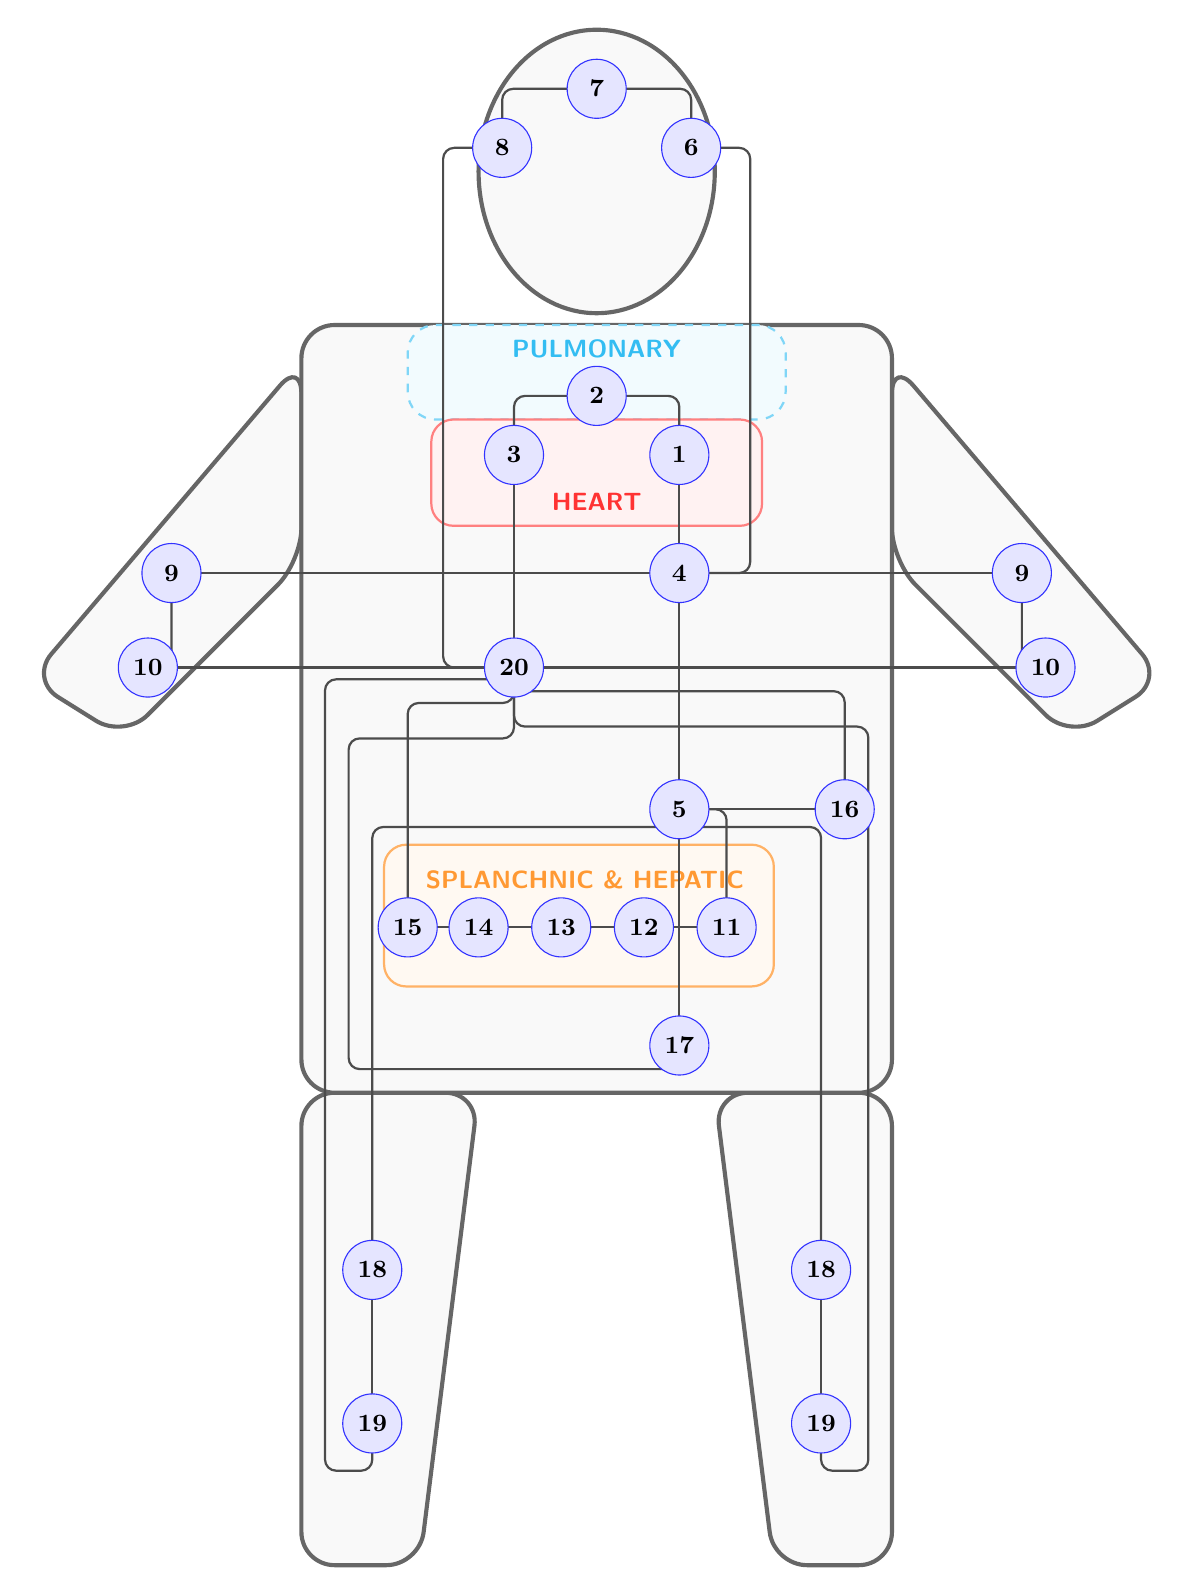
\begin{tikzpicture}[scale=1.5, x=1cm, y=1cm]

        % ==========================================
        % 1. SYMMETRICAL BODY OUTLINE
        % ==========================================
        
        % Arms (Right Arm = Viewer's Left, Left Arm = Viewer's Right)
        \draw[organ] (-2.5, 7.2) -- (-4.8, 4.5) -- (-4.0, 4.0) -- (-2.5, 5.5) -- cycle; 
        \draw[organ] (2.5, 7.2) -- (4.8, 4.5) -- (4.0, 4.0) -- (2.5, 5.5) -- cycle;  
        
        % Legs (Torso meets legs at y=1.0)
        \draw[organ] (-1.0, 1.0) -- (-1.5, -3.0) -- (-2.5, -3.0) -- (-2.5, 1.0) -- cycle; 
        \draw[organ] (1.0, 1.0) -- (1.5, -3.0) -- (2.5, -3.0) -- (2.5, 1.0) -- cycle;  

        % Torso (Extended down to y=1.0)
        \draw[organ] (-2.5, 1.0) rectangle (2.5, 7.5);
        
        % Head
        \draw[organ] (0, 8.8) ellipse (1.0cm and 1.2cm);


        % ==========================================
        % 2. INTERNAL ORGAN REGIONS
        % ==========================================
        
        % Lungs
        \draw[lungbox] (-1.6, 6.7) rectangle (1.6, 7.5);
        \node[label, text=cyan!80] at (0, 7.3) {PULMONARY};

        % Heart 
        \draw[heartbox] (-1.4, 5.8) rectangle (1.4, 6.7);
        \node[label, text=red!80] at (0, 6.0) {HEART}; 

        % Splanchnic/Hepatic Box
        \draw[organbox] (-1.8, 1.9) rectangle (1.5, 3.1);
        \node[label, text=orange!80] at (-0.1, 2.8) {SPLANCHNIC \& HEPATIC}; 


        % ==========================================
        % 3. VESSEL ROUTING (Drawn first so nodes sit on top)
        % ==========================================
        
        % Heart & Central Loop (Node 2 routing moved down to 6.9)
        \draw[vessel] (0.7, 6.4) -- (0.7, 5.4); % 1 -> 4
        \draw[vessel] (0.7, 5.4) -- (0.7, 3.4); % 4 -> 5
        \draw[vessel] (-0.7, 4.6) -- (-0.7, 6.4); % 20 -> 3
        \draw[vessel] (-0.7, 6.4) |- (0.0, 6.9);  % 3 -> 2
        \draw[vessel] (0.0, 6.9) -| (0.7, 6.4);   % 2 -> 1

        % Head
        \draw[vessel] (0.7, 5.4) -- (1.3, 5.4) -- (1.3, 9.0) -- (0.8, 9.0); % 4 -> 6
        \draw[vessel] (0.8, 9.0) |- (0.0, 9.5); % 6 -> 7
        \draw[vessel] (0.0, 9.5) -| (-0.8, 9.0); % 7 -> 8
        \draw[vessel] (-0.8, 9.0) -- (-1.3, 9.0) -- (-1.3, 4.6) -- (-0.7, 4.6); % 8 -> 20

        % Left Arm (Viewer's Right)
        \draw[vessel] (0.7, 5.4) -- (3.6, 5.4); % 4 -> 9L
        \draw[vessel] (3.6, 5.4) |- (3.8, 4.6); % 9L -> 10L
        \draw[vessel] (3.8, 4.6) -- (-0.7, 4.6); % 10L -> 20

        % Right Arm (Viewer's Left)
        \draw[vessel] (0.7, 5.4) -- (-3.6, 5.4); % 4 -> 9R
        \draw[vessel] (-3.6, 5.4) |- (-3.8, 4.6); % 9R -> 10R
        \draw[vessel] (-3.8, 4.6) -- (-0.7, 4.6); % 10R -> 20

        % Abdominal / Splanchnic Chain
        \draw[vessel] (0.7, 3.4) -| (1.1, 2.4); % 5 -> 11
        \draw[vessel] (1.1, 2.4) -- (0.4, 2.4); % 11 -> 12
        \draw[vessel] (0.4, 2.4) -- (-0.3, 2.4); % 12 -> 13
        \draw[vessel] (-0.3, 2.4) -- (-1.0, 2.4); % 13 -> 14
        \draw[vessel] (-1.0, 2.4) -- (-1.6, 2.4); % 14 -> 15
        \draw[vessel] (-1.6, 2.4) -- (-1.6, 4.3) -- (-0.7, 4.3) -- (-0.7, 4.6); % 15 -> 20

        % Renal
        \draw[vessel] (0.7, 3.4) -- (2.1, 3.4); % 5 -> 16
        \draw[vessel] (2.1, 3.4) -- (2.1, 4.4) -- (-0.7, 4.4) -- (-0.7, 4.6); % 16 -> 20

        % Pelvic
        \draw[vessel] (0.7, 3.4) -- (0.7, 1.4); % 5 -> 17
        % Route return vessel up the left torso wall to avoid splanchnic nodes
        \draw[vessel] (0.7, 1.4) -- (0.7, 1.2) -- (-2.1, 1.2) -- (-2.1, 4.0) -- (-0.7, 4.0) -- (-0.7, 4.6); % 17 -> 20

        % Left Leg (Viewer's Right)
        \draw[vessel] (0.7, 3.4) -- (0.7, 3.25) -- (1.9, 3.25) -- (1.9, -0.5); % 5 -> 18L
        \draw[vessel] (1.9, -0.5) -- (1.9, -1.8); % 18L -> 19L
        \draw[vessel] (1.9, -1.8) -- (1.9, -2.2) -- (2.3, -2.2) -- (2.3, 4.1) -- (-0.7, 4.1) -- (-0.7, 4.6); % 19L -> 20

        % Right Leg (Viewer's Left)
        \draw[vessel] (0.7, 3.4) -- (0.7, 3.25) -- (-1.9, 3.25) -- (-1.9, -0.5); % 5 -> 18R
        \draw[vessel] (-1.9, -0.5) -- (-1.9, -1.8); % 18R -> 19R
        \draw[vessel] (-1.9, -1.8) -- (-1.9, -2.2) -- (-2.3, -2.2) -- (-2.3, 4.5) -- (-0.7, 4.5) -- (-0.7, 4.6); % 19R -> 20


        % ==========================================
        % 4. NODES (Drawn last to overlay perfectly)
        % ==========================================
        
        % Head
        \node[zone] (Z6)  at ( 0.8, 9.0) {6};
        \node[zone] (Z7)  at ( 0.0, 9.5) {7};
        \node[zone] (Z8)  at (-0.8, 9.0) {8};

        % Heart & Lungs (Node 2 moved down to 6.9)
        \node[zone] (Z1)  at ( 0.7, 6.4) {1};
        \node[zone] (Z3)  at (-0.7, 6.4) {3};
        \node[zone] (Z2)  at ( 0.0, 6.9) {2};

        % Central Nodes
        \node[zone] (Z4)  at ( 0.7, 5.4) {4};
        \node[zone] (Z20) at (-0.7, 4.6) {20};
        \node[zone] (Z5)  at ( 0.7, 3.4) {5};
        \node[zone] (Z17) at ( 0.7, 1.4) {17}; 

        % Splanchnic Box
        \node[zone] (Z11) at ( 1.1, 2.4) {11};
        \node[zone] (Z12) at ( 0.4, 2.4) {12};
        \node[zone] (Z13) at (-0.3, 2.4) {13};
        \node[zone] (Z14) at (-1.0, 2.4) {14};
        \node[zone] (Z15) at (-1.6, 2.4) {15};

        % Renal
        \node[zone] (Z16) at ( 2.1, 3.4) {16};

        % Upper Limbs
        \node[zone] (Z9L)  at ( 3.6, 5.4) {9};
        \node[zone] (Z10L) at ( 3.8, 4.6) {10};
        \node[zone] (Z9R)  at (-3.6, 5.4) {9};
        \node[zone] (Z10R) at (-3.8, 4.6) {10};

        % Lower Limbs
        \node[zone] (Z18L) at ( 1.9, -0.5) {18};
        \node[zone] (Z19L) at ( 1.9, -1.8) {19};
        \node[zone] (Z18R) at (-1.9, -0.5) {18};
        \node[zone] (Z19R) at (-1.9, -1.8) {19};

    \end{tikzpicture}

    \vfill

    % ==========================================
    % 5. CLEAN LEGEND
    % ==========================================
    \begin{minipage}{\textwidth}
    \centering
    \textbf{\Large Zone Legend (20-Zone Model)} \\[0.4cm]
    \begin{small}
    \begin{tabular}{rlrlrlrl}
        \textbf{1} & Left Heart & \textbf{6} & Head Arterial & \textbf{11} & Splanchnic Art. & \textbf{16} & Renal Circ. \\
        \textbf{2} & Pulmonary Circ. & \textbf{7} & Head Microcirc. & \textbf{12} & Intest. Microcirc. & \textbf{17} & Pelvic Arterial \\
        \textbf{3} & Right Heart & \textbf{8} & Head Venous & \textbf{13} & Portal Venous & \textbf{18} & Lower Limb Art. \\
        \textbf{4} & Thoracic Aorta & \textbf{9} & Upper Limb Art. & \textbf{14} & Liver Microcirc. & \textbf{19} & Lower Limb Micro. \\
        \textbf{5} & Abdominal Aorta & \textbf{10} & Upper Limb Ven. & \textbf{15} & Hepatic Vein & \textbf{20} & Systemic Return \\
    \end{tabular}
    \end{small}
    \end{minipage}

\end{center}

\newpage
\subsection{Balanced 14-Zone Mapping of 94 Vessels}
\begin{table}[H]
\centering
\begin{tabular}{|c|p{10cm}|}
\hline
\textbf{Zone} & \textbf{Vessel IDs} \\
\hline

1  & 1, 2, 57, 58, 61, 94 \\ \hline
2  & 3, 4, 8, 10, 12, 13, 18 \\ \hline
3  & 5, 6, 14, 16, 20, 22, 28 \\ \hline
4  & 7, 9, 64, 65, 80, 81, 82, 83 \\ \hline
5  & 25, 32, 35, 36, 37, 76, 77 \\ \hline
6  & 15, 17, 39, 40, 74, 75, 86 \\ \hline
7  & 38, 41, 42, 43, 44, 45, 46 \\ \hline
8  & 47, 49, 51, 52, 54, 56 \\ \hline
9  & 48, 50, 53, 55, 59, 60 \\ \hline
10 & 62, 63, 66, 67, 68, 69, 70, 71 \\ \hline
11 & 72, 73, 78, 79, 85, 87 \\ \hline
12 & 88, 89, 90, 91, 92, 93 \\ \hline
13 & 19, 26, 30, 31, 34, 84 \\ \hline
14 & 11, 21, 23, 24, 27, 29, 33 \\ \hline

\end{tabular}
\caption{Balanced Distribution of 94 Vessels into 14 Zones}
\end{table}

\begin{table}[h]
\centering
\resizebox{\textwidth}{!}{%
\begin{tabular}{|c|l|c|c|c|c|}
\hline
\textbf{Zone} & \textbf{Zone Name} & \textbf{Press (mmHg)} & \textbf{pH} & \textbf{SO$_2$ (\%)} & \textbf{Temp (\si{\degreeCelsius})} \\
\hline
1 & Heart + Pulmonary Circulation & $0--12$ & $7.35--7.45$ & $70--99$ & $36.8--37.2$ \\ \hline
2 & Thoracic Aorta & $80--120$ & $7.35--7.45$ & $97--99$ & $36.8--37.2$ \\ \hline
3 & Upper Limb Arteries & $70--120$ & $7.35--7.45$ & $97--99$ & $36.8--37.2$ \\ \hline
4 & Head Arteries + Veins & $2--110$ & $7.35--7.45$ & $60--85$ & $36.5--37.2$ \\ \hline
5 & Splanchnic Arteries + Liver & $20--120$ & $7.35--7.45$ & $75--99$ & $36.8--37.8$ \\ \hline
6 & Kidneys + Small Mesenteric & $20--35$ & $7.35--7.40$ & $80--90$ & $36.8--37.0$ \\ \hline
7 & Pelvic Arteries & $70--110$ & $7.35--7.45$ & $97--99$ & $36.8--37.2$ \\ \hline
8 & Pelvis & $35--50$ & $7.35--7.45$ & $95--97$ & $36.0--36.8$ \\ \hline
9 & Lower Limb Arteries & $70--110$ & $7.35--7.45$ & $97--99$ & $36.5--37.2$ \\ \hline
10 & Lower Limb Venules & $2--15$ & $7.35--7.38$ & $70--75$ & $35.0--36.5$ \\ \hline
11 & Systemic Deep Veins & $2--6$ & $7.35--7.38$ & $70--75$ & $35.0--36.8$ \\ \hline
12 & Hepatic & $2--15$ & $7.35--7.38$ & $65--80$ & $37.0--38.0$ \\ \hline
13 & Abdominal Aorta + Mesenteric & $80--120$ & $7.35--7.45$ & $80--99$ & $36.8--37.2$ \\ \hline
14 & Misc Upper Body Arteries & $80--120$ & $7.35--7.45$ & $97--99$ & $36.8--37.2$ \\ \hline

\end{tabular}%
}
\caption{Physiological Parameters Aggregated per Balanced 14-Zone Mapping}
\label{tab:balanced_14zones}
\end{table}

\newpage
\begin{center}
    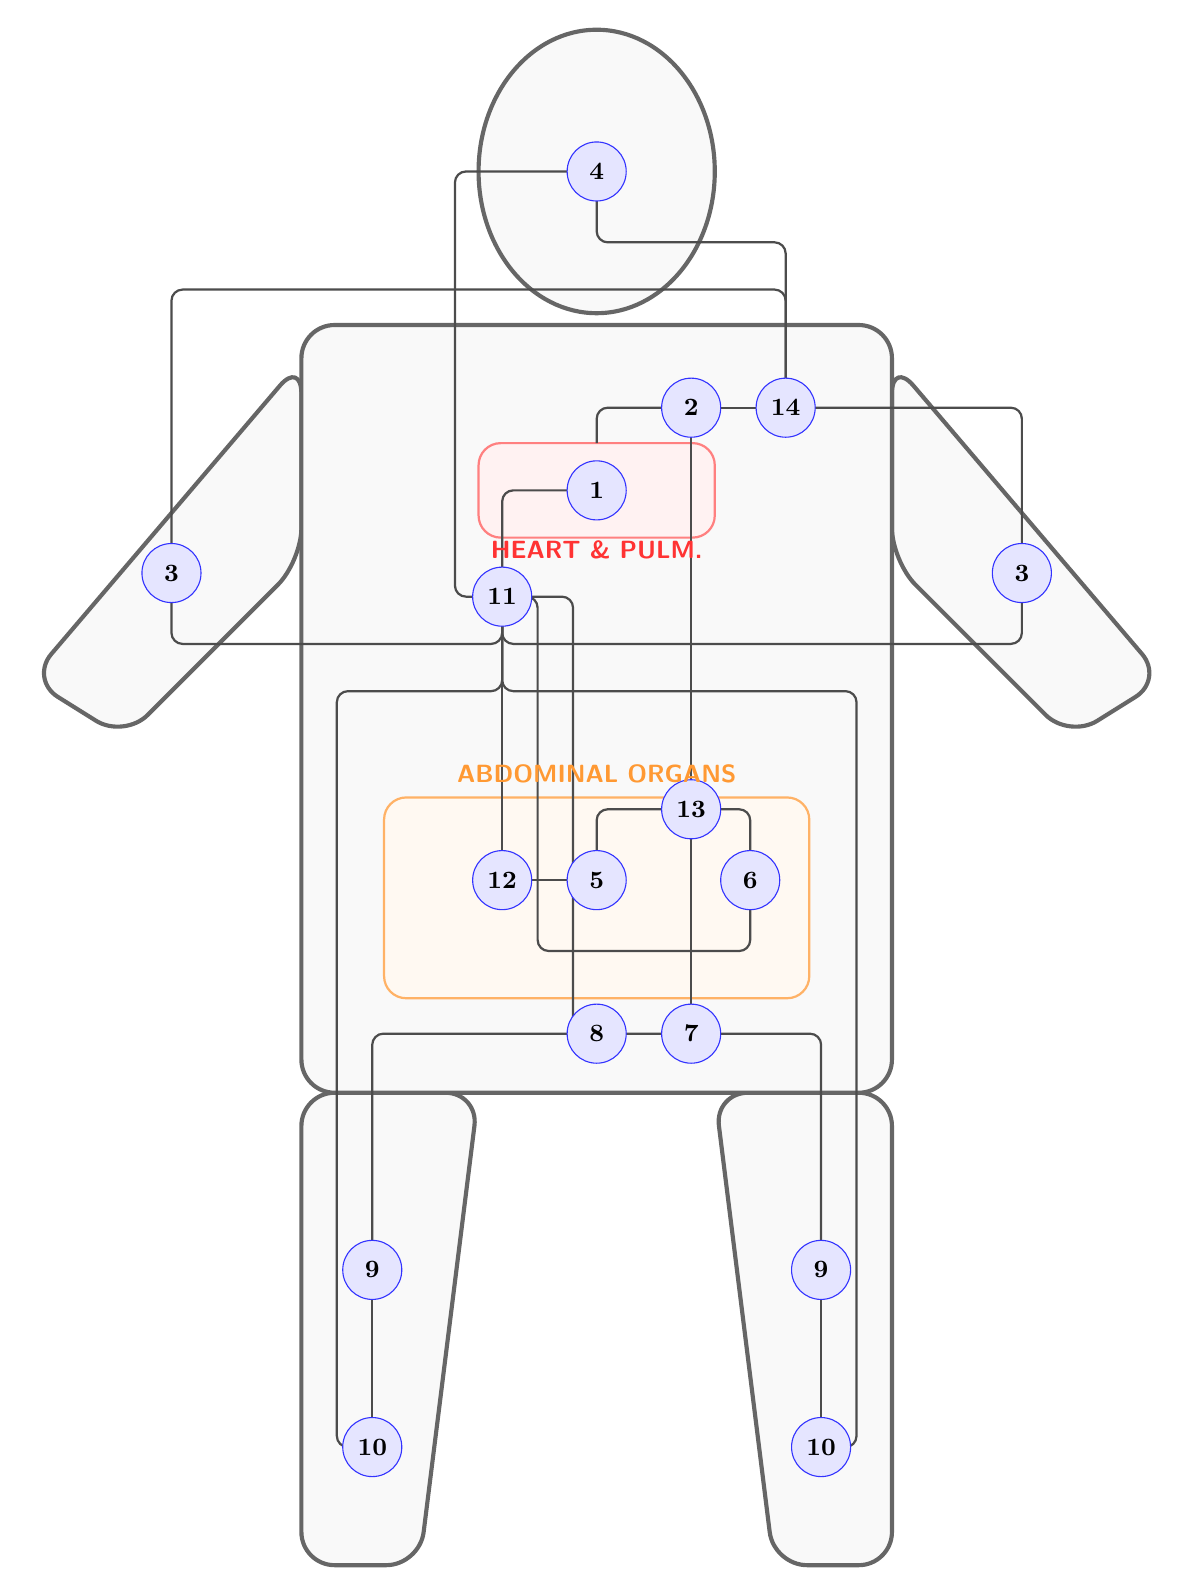
\begin{tikzpicture}[scale=1.5, x=1cm, y=1cm]

        % ==========================================
        % 1. SYMMETRICAL BODY OUTLINE
        % ==========================================
        
        % Arms
        \draw[organ] (-2.5, 7.2) -- (-4.8, 4.5) -- (-4.0, 4.0) -- (-2.5, 5.5) -- cycle; 
        \draw[organ] (2.5, 7.2) -- (4.8, 4.5) -- (4.0, 4.0) -- (2.5, 5.5) -- cycle;  
        
        % Legs
        \draw[organ] (-1.0, 1.0) -- (-1.5, -3.0) -- (-2.5, -3.0) -- (-2.5, 1.0) -- cycle; 
        \draw[organ] (1.0, 1.0) -- (1.5, -3.0) -- (2.5, -3.0) -- (2.5, 1.0) -- cycle;  

        % Torso
        \draw[organ] (-2.5, 1.0) rectangle (2.5, 7.5);
        
        % Head
        \draw[organ] (0, 8.8) ellipse (1.0cm and 1.2cm);


        % ==========================================
        % 2. INTERNAL ORGAN REGIONS
        % ==========================================
        
        % Heart Area
        \draw[heartbox] (-1.0, 5.7) rectangle (1.0, 6.5);
        % Abdominal Area
        \draw[organbox] (-1.8, 1.8) rectangle (1.8, 3.5);


        % ==========================================
        % 3. VESSEL ROUTING (Drawn first under nodes)
        % ==========================================
        
        % --- Arterial Outflow (from Heart 1) ---
        % To Thoracic Aorta (2) and Misc Upper (14)
        \draw[vessel] (0.0, 6.5) -- (0.0, 6.8) -- (0.8, 6.8); % 1 -> 2
        \draw[vessel] (0.8, 6.8) -- (1.6, 6.8); % 2 -> 14
        
        % Aorta (2) down to Abdominal Aorta (13)
        \draw[vessel] (0.8, 6.8) -- (0.8, 3.4); % 2 -> 13

        % --- Upper Body Distribution ---
        % To Head (4)
        \draw[vessel] (1.6, 6.8) -- (1.6, 8.2) -- (0.0, 8.2) -- (0.0, 8.8); % 14 -> 4
        % To Arms (3)
        \draw[vessel] (1.6, 6.8) -- (3.6, 6.8) -- (3.6, 5.4); % 14 -> 3L
        \draw[vessel] (1.6, 6.8) -- (1.6, 7.8) -- (-3.6, 7.8) -- (-3.6, 5.4); % 14 -> 3R

        % --- Abdominal Distribution (from Abd Aorta 13) ---
        \draw[vessel] (0.8, 3.4) -- (0.0, 3.4) -- (0.0, 2.8); % 13 -> 5 (Splanchnic)
        \draw[vessel] (0.8, 3.4) -- (1.3, 3.4) -- (1.3, 2.8); % 13 -> 6 (Kidneys)
        \draw[vessel] (0.8, 3.4) -- (0.8, 1.5); % 13 -> 7 (Pelvic Art)
        
        % --- Lower Limb Distribution ---
        \draw[vessel] (0.8, 1.5) -- (1.9, 1.5) -- (1.9, -0.5); % 7 -> 9L (Leg Art)
        \draw[vessel] (0.8, 1.5) -- (-1.9, 1.5) -- (-1.9, -0.5); % 7 -> 9R (Leg Art)

        % ==========================================
        % Venous Return Paths (Collecting to Systemic Veins 11)
        % ==========================================
        
        % From Head (4)
        \draw[vessel] (0.0, 8.8) -- (-1.2, 8.8) -- (-1.2, 5.2) -- (-0.8, 5.2); % 4 -> 11
        % From Arms (3)
        \draw[vessel] (3.6, 5.4) -- (3.6, 4.8) -- (-0.8, 4.8) -- (-0.8, 5.2); % 3L -> 11
        \draw[vessel] (-3.6, 5.4) -- (-3.6, 4.8) -- (-0.8, 4.8) -- (-0.8, 5.2); % 3R -> 11
        
        % Abdominal Returns
        \draw[vessel] (0.0, 2.8) -- (-0.8, 2.8); % 5 (Splanc) -> 12 (Hepatic)
        \draw[vessel] (-0.8, 2.8) -- (-0.8, 5.2); % 12 (Hepatic) -> 11
        \draw[vessel] (1.3, 2.8) -- (1.3, 2.2) -- (-0.5, 2.2) -- (-0.5, 5.2) -- (-0.8, 5.2); % 6 (Kidneys) -> 11

        % Pelvic/Lower Returns
        \draw[vessel] (0.8, 1.5) -- (0.0, 1.5); % 7 (Pelvic Art) -> 8 (Pelvis)
        \draw[vessel] (0.0, 1.5) -- (-0.2, 1.5) -- (-0.2, 5.2) -- (-0.8, 5.2); % 8 -> 11
        
        \draw[vessel] (1.9, -0.5) -- (1.9, -2.0); % 9L -> 10L
        \draw[vessel] (-1.9, -0.5) -- (-1.9, -2.0); % 9R -> 10R
        % Leg veins to systemic
        \draw[vessel] (1.9, -2.0) -- (2.2, -2.0) -- (2.2, 4.4) -- (-0.8, 4.4) -- (-0.8, 5.2); % 10L -> 11
        \draw[vessel] (-1.9, -2.0) -- (-2.2, -2.0) -- (-2.2, 4.4) -- (-0.8, 4.4) -- (-0.8, 5.2); % 10R -> 11

        % Final Return to Heart
        \draw[vessel] (-0.8, 5.2) -- (-0.8, 6.1) -- (0.0, 6.1); % 11 -> 1


        % ==========================================
        % 4. NODES (Drawn last)
        % ==========================================
        
        % Head
        \node[zone] (Z4) at (0.0, 8.8) {4};

        % Chest Area
        \node[zone] (Z1) at (0.0, 6.1) {1}; % Heart+Pulm
        \node[zone] (Z2) at (0.8, 6.8) {2}; % Thoracic Aorta
        \node[zone] (Z14) at (1.6, 6.8) {14}; % Misc Upper Art
        \node[zone] (Z11) at (-0.8, 5.2) {11}; % Systemic Veins

        % Arms
        \node[zone] (Z3L) at (3.6, 5.4) {3};
        \node[zone] (Z3R) at (-3.6, 5.4) {3};

        % Abdomen
        \node[zone] (Z13) at (0.8, 3.4) {13}; % Abd Aorta
        \node[zone] (Z5) at (0.0, 2.8) {5}; % Splanchnic+Liv
        \node[zone] (Z12) at (-0.8, 2.8) {12}; % Hepatic
        \node[zone] (Z6) at (1.3, 2.8) {6}; % Kidneys

        % Pelvis
        \node[zone] (Z7) at (0.8, 1.5) {7}; % Pelvic Art
        \node[zone] (Z8) at (0.0, 1.5) {8}; % Pelvis

        % Legs
        \node[zone] (Z9L) at (1.9, -0.5) {9}; % Art L
        \node[zone] (Z10L) at (1.9, -2.0) {10}; % Ven L
        \node[zone] (Z9R) at (-1.9, -0.5) {9}; % Art R
        \node[zone] (Z10R) at (-1.9, -2.0) {10}; % Ven R
        
        % Labels
        \node[label, text=red!80] at (0, 5.6) {HEART \& PULM.};
        \node[label, text=orange!80] at (0, 3.7) {ABDOMINAL ORGANS};

    \end{tikzpicture}

    \vfill

    % ==========================================
    % 5. NEW LEGEND (14 ZONES)
    % ==========================================
    \begin{minipage}{\textwidth}
    \centering
    \textbf{\Large Zone Legend (14-Zone Model)} \\[0.4cm]
    \begin{small}
    \begin{tabular}{rlrl}
        \textbf{1} & Heart + Pulmonary Circulation & \textbf{8} & Pelvis \\
        \textbf{2} & Thoracic Aorta & \textbf{9} & Lower Limb Arteries \\
        \textbf{3} & Upper Limb Arteries & \textbf{10} & Lower Limb Venules \\
        \textbf{4} & Head Arteries + Veins & \textbf{11} & Systemic Deep Veins \\
        \textbf{5} & Splanchnic Arteries + Liver & \textbf{12} & Hepatic \\
        \textbf{6} & Kidneys + Small Mesenteric & \textbf{13} & Abdominal Aorta + Mesenteric \\
        \textbf{7} & Pelvic Arteries & \textbf{14} & Misc Upper Body Arteries \\
    \end{tabular}
    \end{small}
    \end{minipage}

\end{center}

\subsection{Rationale for the use of the 20-Zone Hybrid Mapping}

While a balanced 14-zone mapping (Table \ref{tab:balanced_14zones}) was initially considered to mitigate the uneven spatial distribution of the nanobot swarm, ensuring a higher and more consistent sampling frequency across all regions, the 20-zone hybrid mapping (Table \ref{tab:hybrid_zones}) was selected as the basis for this framework. The superiority of the 20-zone model is based on three factors:

\begin{itemize}
    \item \textbf{Variance Reduction:} For an anomaly detector to identify subtle, early-stage pathological drift, the baseline physiological variance of the target zone must be as narrow as possible. The 14-zone model inflates this variance by merging functionally distinct vessels. For example, Zone 4 in the 14-zone model combines "Head Arteries + Veins", resulting in a baseline oxygen saturation ($SO_2$) interval of 60--85\% and a pressure interval of 2--110 mmHg. A Kalman filter calibrated to such a chaotic baseline would be entirely blind to early hypoxic or hypotensive events. The 20-zone model separates these into Head Arterial, Head Microcirculation, and Head Venous, creating tight, mathematically stable baselines.
    
    \item \textbf{Diagnostic Granularity for Capillary Pathologies:} Many of the most critical pathologies that will be simulated, originate in highly specific capillary beds or localized venous segments. Grouping macro-arteries with microcirculation (as seen in the 14-zone model's "Kidneys + Small Mesenteric" zone) dilutes the localized pathological signal with overwhelming volumes of healthy arterial data, drastically increasing the False Negative rate.
    
    \item \textbf{Kalman Filter Sensitivity vs. Sampling Frequency Trade-off:} While the 20-zone model results in an uneven distribution of raw data pings (e.g., central aortic zones receive more visits than peripheral extremity microcirculation), the detection framework compensates for this computationally rather than anatomically. It is clinically preferable to wait slightly longer to gather sufficient data in a precisely mapped 20-zone model than to receive immediate, but physiologically meaningless, data from a heavily merged 14-zone model.
\end{itemize}

\newpage 
\section{Sample Size and Reliability Determination}
\subsection{Data Presentation}

The raw telemetry collected by the nanobot swarm is inherently stochastic. Crucially, the biological "ground truth" of any anatomical zone is not a static scalar value, but rather a dynamic reading naturally drawn from a specific homeostatic interval (e.g., a healthy arterial pH naturally fluctuating between $7.35$ and $7.45$, as detailed in Table \ref{tab:hybrid_zones}). Therefore, the raw data stream represents a complex mixture of distributions: the natural physiological variance acts as the base distribution, upon which simulated hardware and spatial errors are mathematically overlaid. 

As illustrated in Figure \ref{fig:noise_domains}, the corruption of this already dynamic signal manifests in two distinct domains. In the time domain (Figure \ref{fig:noise_domains}A), continuous, high-frequency fluctuations represent hardware measurement jitter ($\beta$). Concurrently, severe and isolated outliers appear when a nanobot experiences a localization error ($\alpha$), incorrectly tagging its anatomical coordinates and reporting a value sampled from an entirely different physiological zone. 

Statistically (Figure \ref{fig:noise_domains}B), these compounded errors severely alter the reliability of the data. The $\beta$ measurement jitter artificially widens the natural physiological interval into a broad Gaussian distribution, heavily reducing the trustworthiness of any single ping. Meanwhile, the $\alpha$ spikes act as discrete samples drawn entirely from outlying physiological distributions (e.g., a colder peripheral venous temperature polluting a warmer central arterial dataset). Because this compound noise overlaps across the hybrid zones, evaluating individual raw pings is highly prone to false positives, necessitating a robust statistical strategy to extract the true pathological baseline.

\begin{figure}[H]
    \centering
    \includegraphics[width=1\linewidth]{Noisy_Raw_Sensor_Data.png}
    \caption{\textbf{Dual-domain visualization of compound stochastic noise in raw nanobot telemetry.} \textbf{(A)} Time-series representation showing how individual sensor pings deviate from the biological ground truth due to $\beta$ jitter (highlighted in blue) and $\alpha$ localization spikes (highlighted in red). \textbf{(B)} Probability Density Function (PDF) illustrating the statistical origin of these errors, where $\beta$ noise widens the theoretical signal (black to blue) and $\alpha$ noise introduces samples from an outlying physiological distribution (red).}
    \label{fig:noise_domains}
\end{figure}

\subsection{Definitions and Sampling Strategy}
To guarantee the reliability of the simulated physiological measurements, we must aggregate noisy raw sensor data. We define the following parameters:

\begin{itemize}
    \item \textbf{$N$ (Smoothing Window Size):} The number of raw, noisy sensor samples that must be aggregated (via median filtering) to produce \textbf{one} single validated output.
    \item \textbf{$V_z$ (Zonal Visits):} The total number of raw measurements taken in a specific physiological zone $z$ over the entire simulation.
\end{itemize}

\subsection{Compound Error (\texorpdfstring{$\epsilon$}{epsilon})}
We define two distinct sources of error that compromise a measurement:
\begin{itemize}
    \item \textbf{$\alpha$ (Localization Error):} The probability that the sensor is assigned to the wrong zone. 
    \item \textbf{$\beta$ (Measurement Error):} The probability that the sensor measures an erroneous value.
\end{itemize}

For a sample to be valid, it must be both correctly localized and correctly measured. The probability of a valid sample is $(1-\alpha)(1-\beta)$.
Consequently, the total effective error rate $\epsilon$ (probability that a sample is invalid for any reason) is:

\begin{equation}
    \epsilon = 1 - (1 - \alpha)(1 - \beta) = \alpha + \beta - \alpha \cdot \beta
\end{equation}

\textit{Constraint:} The majority voting logic (Median) mathematically fails if $\epsilon \geq 0.5$.

\begin{figure}[H]
    \centering
    \includegraphics[width=0.7\linewidth]{Compound_Error.png}
    \caption{\textbf{Theoretical compound error space and statistical aggregation limits.} The contour gradient visualizes the total effective error rate ($\epsilon$) relative to the spatial localization error ($\alpha$) and hardware measurement error ($\beta$). The dashed black line demarcates the critical failure threshold ($\epsilon = 0.5$), dividing the parameter space into a Safe Zone (green) where median-based aggregation remains mathematically valid, and a Failure Zone (red) where invalid data dominates the swarm's signal.}
    \label{fig:compound_error}
\end{figure}

\subsection{A Priori Analysis: Determining Window Size (\textit{N})}
Before running the simulation, we must determine a minimum required window size $N$ that guarantees a target statistical confidence (e.g., $1-\delta$). We derive this using the Chernoff-Hoeffding Bound.

Modeling the majority vote failure condition as $\bar{X} \le 0.5$ (where the expected validity is $p_{valid} = 1-\epsilon$), the probability of failure is bounded by:

\begin{align}
    P(\text{failure}) &\le \exp\left(-2N(p_{valid} - 0.5)^2\right)
\end{align}

Setting $P(\text{failure}) \le \delta$ and solving for $N$, we establish the minimum required samples per validated output:

\begin{equation}
    N = \left\lceil \frac{\ln(1/\delta)}{2 \cdot (0.5 - \epsilon)^2} \right\rceil
\end{equation}

Where $\lceil \cdot \rceil$ denotes the ceiling function. The calculated $N$ is always adjusted up to the nearest odd integer to prevent tie conditions in the median voter.

\begin{table}[H]
    \centering
    \renewcommand{\arraystretch}{1.5}
    \resizebox{\linewidth}{!}{
    \begin{tabular}{|c||c|c|c|c|}
        \hline
        \multirow{2}{*}{\textbf{Error Profile}} & \multicolumn{4}{c|}{\textbf{Required $N$ per Confidence Level ($1 - \delta$)}} \\
        \cline{2-5}
        & \textbf{85\%} ($\delta=0.15$) & \textbf{90\%} ($\delta=0.10$) & \textbf{95\%} ($\delta=0.05$) & \textbf{99\%} ($\delta=0.01$) \\
        \hline
        \hline

        % SO2 SECTION (beta = 2%)
        $\alpha=20\%, \beta=2\%$ & \multirow{2}{*}{$N = \mathbf{13}$} & \multirow{2}{*}{$N = \mathbf{15}$} & \multirow{2}{*}{$N = \mathbf{19}$} & \multirow{2}{*}{$N = \mathbf{29}$} \\
        $\epsilon = 21.6\%$ & & & & \\
        \hline

        % PRESSURE SECTION (beta = 5%)
        $\alpha=20\%, \beta=5\%$ & \multirow{2}{*}{$N = \mathbf{15}$} & \multirow{2}{*}{$N = \mathbf{19}$} & \multirow{2}{*}{$N = \mathbf{23}$} & \multirow{2}{*}{$N = \mathbf{35}$} \\
        $\epsilon = 24.0\%$ & & & & \\
        \hline

        % pH SECTION (beta = 10%)
        $\alpha=20\%, \beta=10\%$ & \multirow{2}{*}{$N = \mathbf{21}$} & \multirow{2}{*}{$N = \mathbf{25}$} & \multirow{2}{*}{$N = \mathbf{31}$} & \multirow{2}{*}{$N = \mathbf{49}$} \\
        $\epsilon = 28.0\%$ & & & & \\
        \hline
    \end{tabular}
    }
    \caption{Minimum window size ($N$) required \textit{a priori} to achieve specific statistical confidence thresholds based on the Hoeffding Bound. Values are strictly rounded up to the nearest odd integer.}
    \label{tab:apriori_confidence_levels}
\end{table}

\subsection{A Posteriori Analysis: Effective Dataset Reliability}
The unequal spatial distribution of the simulation guarantees that while rare zones may only collect exactly $N$ samples, highly frequented zones will gather $V_z \gg N$ samples. Once the simulation is complete, calculating the exact \textit{effective} confidence of the extracted median for any given sample pool requires a more precise probabilistic model than the conservative Hoeffding bound.

\subsubsection{The Binomial Distribution}
Each measurement taken by a nanobot is modeled as an independent Bernoulli trial. Because the final output is determined by a majority vote, the aggregate success of any window follows a Binomial distribution. 

The effective probability that the majority vote fails (i.e., the number of invalid samples meets or exceeds the threshold required to flip the median) is calculated exactly using the Binomial Cumulative Distribution Function (CDF):
\begin{equation}
    P(\text{failure}) = \sum_{k=0}^{\lfloor N/2 \rfloor} \binom{N}{k} (1 - p_{valid})^k (p_{valid})^{N-k}
\end{equation}
The effective confidence of the extracted median value is therefore $1 - P(\text{failure})$.

\subsubsection{Theoretical Bound vs. Exact Probability}
The Hoeffding inequality assumes worst-case continuous variance and does not account for the discrete combinatorial nature of the trials. Consequently, the actual Binomial confidence is mathematically guaranteed to be higher than the Hoeffding prediction. By evaluating the collected data with the Binomial CDF \textit{a posteriori}, we reveal the true reliability of the samples, demonstrating that the empirical confidence significantly exceeds the baseline analytic bound, particularly at smaller sample sizes.

\subsubsection{Boundary Condition: The Even-N Penalty}
A critical boundary condition added to the \textit{a posteriori} evaluation is the handling of even-numbered sample sizes ($V_z$). Majority voting inherently requires a strict majority ($> 50\%$). If a pool has an even number of samples, a 50/50 tie becomes mathematically possible, which fails the strict majority condition and causes a precipitous drop in evaluated confidence. 

To resolve this without discarding valuable data, the evaluation algorithm applies a conservative boundary adjustment: any collected pool where the count is even is evaluated at $N-1$. This effectively discards one redundant sample to force a strict tie-breaking odd integer, maintaining a rigorous worst-case evaluation without an artificial drop in reliability.

\newpage 
\section{Simulations Setup} \label{sec:sim}
In this chapter, we present a series of simulations designed to evaluate the robustness of the binomial confidence metric under varying environmental and sensor conditions. The study is organized into three distinct experimental phases:

\begin{itemize}
    \item \textbf{Section \ref{sec:fixed_beta}: Sensitivity to Localization Error ($\alpha$).} 
    In this section, we adopt fixed sensor measurement errors ($\beta$) based on established literature. We analyze the behavior of the confidence metric across eight localization significance levels, $\alpha \in \{0.01, 0.1, 0.15, 0.2, 0.25, 0.3, 0.35, 0.4\}$, effectively testing the system from $99\%$ down to $60\%$ localization certainty. These tests are conducted for both $15$-minute and $30$-minute simulation windows.

    \item \textbf{Section \ref{sec:double_variation}: Simultaneous Parameter Variation.} 
    We investigate the interaction between both error types by performing a double-variation analysis. This explores the confidence landscape across the full matrix of our parameters: $\alpha \in \{0.01, 0.1, 0.15, 0.2, 0.25, 0.3, 0.35, 0.4\}$ and $\beta \in \{0.01, 0.02, 0.05, 0.10\}$.

    \item \textbf{Section \ref{sec:long_sim_grouped}: Grouped High-Resolution Simulation.} 
    We extend the simulation duration to 24 hours to determine a consistent time series for the $20$-zone grouping layout. For this high-resolution analysis, we fix $\alpha$ and $\beta$ based on the optimal values identified in the previous sections to observe at what point the system reaches an acceptable confidence threshold.
    
    \item \textbf{Section \ref{sec:long_sim}: Plain High-Resolution Simulation.} 
    We extend the simulation duration to 24 hours to determine a consistent time series for the original $94$-zone layout without spatial grouping. For this high-resolution analysis, we fix $\alpha$ and $\beta$ based on the optimal values identified in the previous sections to observe at what point the system reaches an acceptable confidence threshold.
\end{itemize}

\subsection{Simulations with Fixed \texorpdfstring{$\beta$}{beta}} \label{sec:fixed_beta}
Since in the literature there are no universal fixed errors for intravascular nanobots, we define $\beta$ based on the performance of state-of-the-art MEMS and optical biosensors.

\begin{itemize}
    \item \textbf{Blood Pressure ($\beta = 0.05$):} Reflects the anticipated noise from turbulent blood flow and sensor-wall interactions in vivo. While state-of-the-art miniaturized capacitive sensors possess high intrinsic electrical accuracy, this error margin is applied to account for the physical instability of a free-floating nanobot in the circulatory system.
    \begin{itemize}
        \item Oh S, Lee Y, Wang J, et al. Dual-slope capacitance to digital converter integrated in an implantable pressure sensing system. \emph{Symposium on VLSI Circuits Digest of Technical Papers}, 2014.
    \end{itemize}
    \item \textbf{Blood pH ($\beta = 0.10$):} Reflects the anticipated error margin caused by sensor drift and chemical noise in complex biological fluids like blood plasma. While continuous ISFET monitoring is highly effective, it suffers from well-documented hardware limitations, most notably temporal threshold drift and high chemical noise at the insulator-electrolyte interface. This error rate is applied to simulate these physical constraints in vivo.
    \begin{itemize}
        \item Moser N, Lande TS, Toumazou C, Georgiou P. ISFETs in CMOS and emergent trends in chemical sensing: A review. \emph{IEEE Sensors Journal}, 2016.
    \end{itemize}
    \item \textbf{Oxygen Saturation ($SO_2$) ($\beta = 0.02$):} Based on high-precision reflectance oximetry, which maintains error margins strictly below 2\% even in flexible and organic form factors.
    \begin{itemize}
        \item Khan Y et al. A flexible organic reflectance oximeter array. \emph{Proceedings of the National Academy of Sciences (PNAS)}, 2018.
    \end{itemize}
    \item \textbf{Temperature ($\beta = 0.01$):} Reflects the high stability of micro-thermistor and CMOS components, which reliably achieve sub-degree accuracy in physiological ranges.
    \begin{itemize}
        \item Jayaram C, Rao PS. A 0.5-V energy-efficient CMOS temperature sensor with 97.64 pJ/conversion for portable applications. \emph{IEEE Sensors Journal}, 2024.
    \end{itemize}
\end{itemize}
While these state-of-the-art performance metrics are currently derived from external, wearable, or macro-scale implantable biosensors, our simulations operate under the assumption that future intravascular nanodevices will successfully miniaturize these technologies while maintaining equivalent error margins and performance capabilities at the nanoscale.

\newpage 

\subsubsection{15 Minutes Simulation}
\begin{table}[H]
    \centering
    \resizebox{\linewidth}{!}{
    \begin{tabular}{c cccccccc}
        \toprule
        \multirow{2}{*}{\textbf{Zone}} & \multicolumn{8}{c}{\textbf{Binomial Confidence (\%) with Fixed $\beta = 0.05$}} \\
        \cmidrule(lr){2-9}
        & \textbf{$\alpha=0.01$} & \textbf{$\alpha=0.10$} & \textbf{$\alpha=0.15$} & \textbf{$\alpha=0.20$} & \textbf{$\alpha=0.25$} & \textbf{$\alpha=0.30$} & \textbf{$\alpha=0.35$} & \textbf{$\alpha=0.40$} \\
        \midrule
        1 & 100.0000 & 100.0000 & 100.0000 & 100.0000 & 100.0000 & 99.9994 & 99.9415 & 96.6504 \\
        2 & 100.0000 & 100.0000 & 100.0000 & 100.0000 & 100.0000 & 100.0000 & 99.9992 & 99.3489 \\
        3 & 100.0000 & 100.0000 & 100.0000 & 100.0000 & 100.0000 & 99.9999 & 99.9720 & 98.2689 \\
        4 & 100.0000 & 100.0000 & 100.0000 & 100.0000 & 99.9999 & 99.9647 & 99.2343 & 93.6382 \\
        5 & 99.9923 & 99.8970 & 98.3344 & 98.0525 & 94.9601 & 90.9452 & 84.0700 & 68.3446 \\
        6 & 100.0000 & 99.9999 & 99.9980 & 99.9424 & 99.2340 & 97.1676 & 88.5658 & 76.1317 \\
        7 & 100.0000 & 100.0000 & 99.9851 & 99.9590 & 99.6868 & 98.5652 & 92.7810 & 79.2286 \\
        8 & 100.0000 & 100.0000 & 100.0000 & 99.9999 & 99.9812 & 99.8768 & 98.4292 & 89.2253 \\
        9 & 100.0000 & 99.9994 & 99.9946 & 99.9190 & 99.6090 & 96.2540 & 91.6153 & 79.2286 \\
        10 & 100.0000 & 100.0000 & 100.0000 & 100.0000 & 99.9966 & 99.9487 & 99.0077 & 91.3157 \\
        11 & \textbf{98.9801} & 97.5760 & 90.3098 & 85.4848 & 88.9589 & 82.4133 & 67.3006 & 62.9545 \\
        12 & \textbf{98.9801} & \textbf{97.5760} & 94.7678 & 85.4848 & 79.9559 & \textbf{66.5000} & 71.2336 & 60.4314 \\
        13 & 99.9984 & 99.8970 & 97.0777 & 99.0618 & 93.5094 & 89.4032 & 82.6053 & 65.0159 \\
        14 & 99.9621 & \textbf{97.5760} & 94.7678 & \textbf{76.0000} & 85.3059 & 82.4133 & 67.3006 & 62.9545 \\
        15 & 99.9997 & 99.7779 & 99.8048 & 93.8305 & 91.5780 & 89.4032 & 76.8899 & 68.3446 \\
        16 & 99.9621 & 98.9289 & 94.7678 & 93.8305 & 79.9559 & 85.2581 & 76.8899 & 62.9545 \\
        17 & 99.9621 & \textbf{97.5760} & \textbf{80.7500} & 85.4848 & 85.3059 & 73.8516 & 67.3006 & 60.4314 \\
        18 & \textbf{98.9801} & 94.3022 & \textbf{80.7500} & 95.6638 & \textbf{79.9559} & 73.8516 & \textbf{61.7500} & \textbf{57.0000} \\
        19 & 99.9621 & 98.9289 & 94.7678 & 95.8450 & 93.5094 & 85.2581 & 74.3301 & 66.7842 \\
        20 & 100.0000 & 100.0000 & 100.0000 & 100.0000 & 100.0000 & 100.0000 & 99.9752 & 98.5273 \\
        \bottomrule
    \end{tabular}
    }
    \caption{Pressure Confidence comparison for Pressure across Localization Errors ($\alpha$) with fixed $\beta = 0.05$}
\end{table}

\begin{table}[H]
    \centering
    \resizebox{\linewidth}{!}{
    \begin{tabular}{c cccccccc}
        \toprule
        \multirow{2}{*}{\textbf{Zone}} & \multicolumn{8}{c}{\textbf{Blood pH Binomial Confidence (\%) with Fixed $\beta = 0.10$}} \\
        \cmidrule(lr){2-9}
        & \textbf{$\alpha=0.01$} & \textbf{$\alpha=0.10$} & \textbf{$\alpha=0.15$} & \textbf{$\alpha=0.20$} & \textbf{$\alpha=0.25$} & \textbf{$\alpha=0.30$} & \textbf{$\alpha=0.35$} & \textbf{$\alpha=0.40$} \\
        \midrule
        1 & 100.0000 & 100.0000 & 100.0000 & 100.0000 & 99.9999 & 99.9788 & 99.0484 & 86.2438 \\
        2 & 100.0000 & 100.0000 & 100.0000 & 100.0000 & 100.0000 & 100.0000 & 99.9146 & 92.7705 \\
        3 & 100.0000 & 100.0000 & 100.0000 & 100.0000 & 100.0000 & 99.9936 & 99.0484 & 87.6933 \\
        4 & 100.0000 & 100.0000 & 100.0000 & 99.9998 & 99.9845 & 99.6444 & 95.4578 & 79.0247 \\
        5 & 99.9524 & 99.8958 & 99.1884 & 95.5951 & 93.4833 & 87.8709 & 76.3175 & 61.5818 \\
        6 & 100.0000 & 99.9990 & 99.8139 & 99.5393 & 98.1807 & 89.0084 & 82.3866 & 68.8184 \\
        7 & 100.0000 & 99.9983 & 99.8704 & 99.2516 & 98.4385 & 92.4658 & 87.0659 & 68.3478 \\
        8 & 100.0000 & 100.0000 & 100.0000 & 99.9956 & 99.9030 & 99.0074 & 92.6200 & 74.1671 \\
        9 & 100.0000 & 99.9983 & 99.8139 & 99.6377 & 98.4385 & 94.7410 & 83.1776 & 67.8606 \\
        10 & 100.0000 & 100.0000 & 100.0000 & 99.9998 & 99.9640 & 99.4309 & 95.7763 & 78.3202 \\
        11 & 98.9075 & 94.9472 & 86.0281 & \textbf{80.8704} & 75.1781 & \textbf{63.0000} & 62.6272 & \textbf{55.9872} \\
        12 & 96.6947 & \textbf{90.5418} & 94.2462 & \textbf{80.8704} & 75.1781 & 69.0606 & 62.6272 & \textbf{55.9872} \\
        13 & 99.9991 & 99.6972 & 97.4378 & 96.6170 & 86.7636 & 89.0084 & 73.5472 & 64.4902 \\
        14 & 98.9075 & 97.2072 & 91.1668 & \textbf{80.8704} & \textbf{67.5000} & 76.5918 & 65.6331 & 57.4681 \\
        15 & 99.8673 & 99.8228 & 96.1838 & 89.8404 & 90.8066 & 76.5918 & 71.9391 & 58.6942 \\
        16 & 98.9075 & 94.9472 & \textbf{76.5000} & 89.8404 & 75.1781 & 76.5918 & 65.6331 & \textbf{55.9872} \\
        17 & 99.6238 & \textbf{90.5418} & 94.2462 & 89.8404 & 75.1781 & 69.0606 & 62.6272 & 57.4681 \\
        18 & \textbf{89.1000} & 94.9472 & \textbf{76.5000} & \textbf{80.8704} & \textbf{67.5000} & 69.0606 & \textbf{58.5000} & \textbf{55.9872} \\
        19 & 99.8673 & 97.2072 & \textbf{76.5000} & 92.3842 & 86.7636 & 73.2988 & 62.6272 & 57.4681 \\
        20 & 100.0000 & 100.0000 & 100.0000 & 100.0000 & 100.0000 & 99.9883 & 99.5261 & 88.1343 \\
        \bottomrule
    \end{tabular}
    }
    \caption{Confidence comparison for Blood pH across Localization Errors ($\alpha$) with fixed $\beta = 0.10$}
\end{table}

\begin{table}[H]
    \centering
    \resizebox{\linewidth}{!}{
    \begin{tabular}{c cccccccc}
        \toprule
        \multirow{2}{*}{\textbf{Zone}} & \multicolumn{8}{c}{\textbf{Oxygen Saturation Binomial Confidence (\%) with Fixed $\beta = 0.02$}} \\
        \cmidrule(lr){2-9}
        & \textbf{$\alpha=0.01$} & \textbf{$\alpha=0.10$} & \textbf{$\alpha=0.15$} & \textbf{$\alpha=0.20$} & \textbf{$\alpha=0.25$} & \textbf{$\alpha=0.30$} & \textbf{$\alpha=0.35$} & \textbf{$\alpha=0.40$} \\
        \midrule
        1 & 100.0000 & 100.0000 & 100.0000 & 100.0000 & 100.0000 & 100.0000 & 99.9791 & 98.6999 \\
        2 & 100.0000 & 100.0000 & 100.0000 & 100.0000 & 100.0000 & 100.0000 & 100.0000 & 99.9314 \\
        3 & 100.0000 & 100.0000 & 100.0000 & 100.0000 & 100.0000 & 100.0000 & 99.9960 & 99.2429 \\
        4 & 100.0000 & 100.0000 & 100.0000 & 100.0000 & 99.9999 & 99.9969 & 99.8411 & 97.1701 \\
        5 & 100.0000 & 99.9888 & 99.5343 & 99.5508 & 96.6898 & 92.2025 & 86.4389 & 77.1029 \\
        6 & 100.0000 & 100.0000 & 99.9971 & 99.9652 & 99.6679 & 99.0952 & 96.0448 & 86.1334 \\
        7 & 100.0000 & 100.0000 & 99.9984 & 99.9934 & 99.8088 & 99.2364 & 94.7072 & 81.4838 \\
        8 & 100.0000 & 100.0000 & 100.0000 & 100.0000 & 99.9974 & 99.7622 & 99.0919 & 92.4450 \\
        9 & 100.0000 & 100.0000 & 99.9898 & 99.9934 & 99.9157 & 99.0952 & 95.2009 & 86.7557 \\
        10 & 100.0000 & 100.0000 & 100.0000 & 100.0000 & 100.0000 & 99.9919 & 99.7338 & 95.3344 \\
        11 & 99.9997 & \textbf{88.2000} & 96.4313 & \textbf{88.0187} & 91.4765 & 85.5091 & 70.0357 & \textbf{58.8000} \\
        12 & \textbf{99.7389} & 98.6341 & 96.4313 & 95.6638 & \textbf{73.5000} & 81.7911 & \textbf{63.7000} & 70.7864 \\
        13 & 100.0000 & 99.9266 & 99.7573 & 95.6638 & 98.1740 & 93.5760 & 89.1387 & 70.7864 \\
        14 & 99.9747 & 98.6341 & 96.4313 & 97.2987 & 95.5042 & 81.7911 & 74.4308 & 63.0637 \\
        15 & 99.9997 & 99.9266 & 99.8725 & 97.2987 & 93.8441 & 85.5091 & 80.5599 & 74.2804 \\
        16 & 99.9974 & 98.6341 & \textbf{92.5648} & 95.6638 & 82.6544 & 76.6130 & 74.4308 & 68.6647 \\
        17 & \textbf{99.7389} & 98.6341 & \textbf{92.5648} & 98.2954 & 88.0036 & 85.5091 & 77.8184 & 63.0637 \\
        18 & \textbf{99.7389} & 96.1514 & \textbf{92.5648} & 95.6638 & \textbf{73.5000} & \textbf{68.6000} & 70.0357 & 66.1624 \\
        19 & 100.0000 & 99.8091 & 96.4313 & 92.9054 & 82.6544 & 85.5091 & 77.8184 & 68.6647 \\
        20 & 100.0000 & 100.0000 & 100.0000 & 100.0000 & 100.0000 & 100.0000 & 99.9985 & 99.7277 \\
        \bottomrule
    \end{tabular}
    }
    \caption{Confidence comparison for SO$_2$ across Localization Errors ($\alpha$) with fixed $\beta = 0.02$}
\end{table}

\begin{table}[H]
    \centering
    \resizebox{\linewidth}{!}{
    \begin{tabular}{c cccccccc}
        \toprule
        \multirow{2}{*}{\textbf{Zone}} & \multicolumn{8}{c}{\textbf{Temperature Binomial Confidence (\%) with Fixed $\beta = 0.01$}} \\
        \cmidrule(lr){2-9}
        & \textbf{$\alpha=0.01$} & \textbf{$\alpha=0.10$} & \textbf{$\alpha=0.15$} & \textbf{$\alpha=0.20$} & \textbf{$\alpha=0.25$} & \textbf{$\alpha=0.30$} & \textbf{$\alpha=0.35$} & \textbf{$\alpha=0.40$} \\
        \midrule
        1 & 100.0000 & 100.0000 & 100.0000 & 100.0000 & 100.0000 & 100.0000 & 99.9953 & 99.4015 \\
        2 & 100.0000 & 100.0000 & 100.0000 & 100.0000 & 100.0000 & 100.0000 & 100.0000 & 99.9690 \\
        3 & 100.0000 & 100.0000 & 100.0000 & 100.0000 & 100.0000 & 100.0000 & 99.9997 & 99.4481 \\
        4 & 100.0000 & 100.0000 & 100.0000 & 100.0000 & 100.0000 & 99.9984 & 99.7230 & 97.4318 \\
        5 & 100.0000 & 99.9828 & 99.2819 & 93.5752 & 92.2314 & 86.4707 & 84.0101 & 74.0091 \\
        6 & 100.0000 & 100.0000 & 99.9998 & 99.9856 & 99.9682 & 98.2433 & 93.0667 & 87.7323 \\
        7 & 100.0000 & 100.0000 & 99.9998 & 99.9997 & 99.8176 & 98.5446 & 97.0547 & 89.4565 \\
        8 & 100.0000 & 100.0000 & 100.0000 & 100.0000 & 99.9986 & 99.9425 & 99.3417 & 92.4850 \\
        9 & 100.0000 & 99.9999 & 99.9969 & 99.9775 & 99.5550 & 99.5172 & 95.9686 & 87.0827 \\
        10 & 100.0000 & 100.0000 & 100.0000 & 100.0000 & 99.9998 & 99.9898 & 99.6952 & 96.3643 \\
        11 & \textbf{98.0100} & 96.6947 & 93.2597 & 97.6913 & \textbf{83.5229} & \textbf{82.7536} & \textbf{70.9340} & 72.0768 \\
        12 & 99.8828 & \textbf{89.1000} & 93.2597 & 93.5752 & \textbf{83.5229} & \textbf{82.7536} & 78.9303 & 69.8510 \\
        13 & 100.0000 & 99.9977 & 99.6452 & 99.4533 & 96.0610 & 93.0122 & 84.0101 & 75.7179 \\
        14 & 99.9995 & 98.9075 & 99.2819 & 96.1860 & 88.8417 & 86.4707 & 81.7125 & 72.0768 \\
        15 & 100.0000 & 99.9524 & 99.2819 & 99.1233 & 97.1555 & 86.4707 & 85.9429 & 75.7179 \\
        16 & 99.9924 & \textbf{89.1000} & 99.2819 & 97.6913 & 96.0610 & 86.4707 & 75.4653 & 67.2141 \\
        17 & 99.9924 & 96.6947 & 96.9048 & 93.5752 & 88.8417 & \textbf{82.7536} & 75.4653 & 67.2141 \\
        18 & \textbf{98.0100} & \textbf{89.1000} & \textbf{84.1500} & \textbf{88.8206} & 88.8417 & \textbf{82.7536} & \textbf{70.9340} & \textbf{63.9339} \\
        19 & 100.0000 & 98.9075 & 99.6452 & 97.6913 & \textbf{83.5229} & 89.2386 & 84.0101 & 74.0091 \\
        20 & 100.0000 & 100.0000 & 100.0000 & 100.0000 & 100.0000 & 100.0000 & 99.9995 & 99.8336 \\
        \bottomrule
    \end{tabular}
    }
    \caption{Confidence comparison for Temperature across Localization Errors ($\alpha$) with fixed $\beta = 0.01$ (15 Minute Simulation)}
\end{table}


\subsubsection{30 Minutes Simulation}

\begin{table}[H]
    \centering
    \resizebox{\linewidth}{!}{
    \begin{tabular}{c ccccccccc}
        \toprule
        \multirow{2}{*}{\textbf{Zone}} & \multicolumn{9}{c}{\textbf{Pressure Binomial Confidence (\%) with Fixed $\beta = 0.05$}} \\
        \cmidrule(lr){2-10}
        & \textbf{$\alpha=0.01$} & \textbf{$\alpha=0.05$} & \textbf{$\alpha=0.10$} & \textbf{$\alpha=0.15$} & \textbf{$\alpha=0.20$} & \textbf{$\alpha=0.25$} & \textbf{$\alpha=0.30$} & \textbf{$\alpha=0.35$} & \textbf{$\alpha=0.40$} \\
        \midrule
        1 & 100.0000 & 100.0000 & 100.0000 & 100.0000 & 100.0000 & 100.0000 & 100.0000 & 99.9995 & 99.3633 \\
        2 & 100.0000 & 100.0000 & 100.0000 & 100.0000 & 100.0000 & 100.0000 & 100.0000 & 100.0000 & 99.9821 \\
        3 & 100.0000 & 100.0000 & 100.0000 & 100.0000 & 100.0000 & 100.0000 & 100.0000 & 100.0000 & 99.8302 \\
        4 & 100.0000 & 100.0000 & 100.0000 & 100.0000 & 100.0000 & 100.0000 & 99.9999 & 99.9663 & 98.0098 \\
        5 & 100.0000 & 100.0000 & 99.9519 & 99.9752 & 99.3443 & 98.7916 & 96.2540 & 89.4359 & 77.7634 \\
        6 & 100.0000 & 100.0000 & 100.0000 & 100.0000 & 99.9993 & 99.9768 & 99.7004 & 95.9370 & 86.1102 \\
        7 & 100.0000 & 100.0000 & 100.0000 & 100.0000 & 99.9999 & 99.9966 & 99.8602 & 97.8071 & 86.5067 \\
        8 & 100.0000 & 100.0000 & 100.0000 & 100.0000 & 100.0000 & 100.0000 & 99.9973 & 99.7056 & 95.0507 \\
        9 & 100.0000 & 100.0000 & 100.0000 & 100.0000 & 99.9998 & 99.9877 & 99.8414 & 98.0823 & 87.6147 \\
        10 & 100.0000 & 100.0000 & 100.0000 & 100.0000 & 100.0000 & 100.0000 & 99.9996 & 99.8916 & 97.0284 \\
        11 & 99.9923 & 99.9208 & 99.7779 & \textbf{94.7678} & 95.8450 & 88.9589 & 87.5396 & 76.8899 & 68.3446 \\
        12 & \textbf{98.9801} & 99.9208 & \textbf{97.5760} & 99.6699 & 99.0618 & 88.9589 & 82.4133 & \textbf{74.3301} & 68.3446 \\
        13 & 100.0000 & 100.0000 & 100.0000 & 99.9851 & 99.9424 & 98.4780 & 96.7448 & 86.5501 & 75.2420 \\
        14 & 99.9984 & 99.9991 & 99.7779 & 99.8048 & 98.0525 & 96.9117 & 92.2334 & 76.8899 & \textbf{65.0159} \\
        15 & 100.0000 & 99.9991 & 99.9949 & 99.9309 & 99.5401 & 97.5678 & 95.6828 & 86.5501 & 74.2951 \\
        16 & 99.9621 & 99.9208 & 99.5159 & 99.4385 & 97.1678 & 91.5780 & 89.4032 & 79.0665 & 71.0234 \\
        17 & 99.9984 & 99.7519 & \textbf{97.5760} & \textbf{94.7678} & \textbf{93.8305} & 88.9589 & 85.2581 & 79.0665 & 66.7842 \\
        18 & 99.9923 & \textbf{99.2034} & \textbf{97.5760} & \textbf{94.7678} & 95.8450 & \textbf{79.9559} & \textbf{78.7648} & \textbf{74.3301} & 66.7842 \\
        19 & 99.9997 & 99.7519 & 99.9893 & 99.8841 & 99.5401 & 96.0638 & 90.9452 & 80.9516 & 72.1968 \\
        20 & 100.0000 & 100.0000 & 100.0000 & 100.0000 & 100.0000 & 100.0000 & 100.0000 & 100.0000 & 99.8509 \\
        \bottomrule
    \end{tabular}
    }
    \caption{Confidence comparison for Pressure across Localization Errors ($\alpha$) with fixed $\beta = 0.05$}
\end{table}

\begin{table}[H]
    \centering
    \resizebox{\linewidth}{!}{
    \begin{tabular}{c cccccccc}
        \toprule
        \multirow{2}{*}{\textbf{Zone}} & \multicolumn{8}{c}{\textbf{Blood pH Binomial Confidence (\%) with Fixed $\beta = 0.10$}} \\
        \cmidrule(lr){2-9}
        & \textbf{$\alpha=0.01$} & \textbf{$\alpha=0.10$} & \textbf{$\alpha=0.15$} & \textbf{$\alpha=0.20$} & \textbf{$\alpha=0.25$} & \textbf{$\alpha=0.30$} & \textbf{$\alpha=0.35$} & \textbf{$\alpha=0.40$} \\
        \midrule
        1 & 100.0000 & 100.0000 & 100.0000 & 100.0000 & 100.0000 & 99.9999 & 99.8430 & 92.0681 \\
        2 & 100.0000 & 100.0000 & 100.0000 & 100.0000 & 100.0000 & 100.0000 & 99.9993 & 98.0491 \\
        3 & 100.0000 & 100.0000 & 100.0000 & 100.0000 & 100.0000 & 100.0000 & 99.9829 & 95.0423 \\
        4 & 100.0000 & 100.0000 & 100.0000 & 100.0000 & 99.9999 & 99.9925 & 99.3829 & 87.2321 \\
        5 & 100.0000 & 99.9635 & 99.4411 & 98.7756 & 97.5220 & 90.0208 & 78.6453 & 68.8184 \\
        6 & 100.0000 & 100.0000 & 99.9995 & 99.9956 & 99.6941 & 97.1198 & 91.0363 & 73.1743 \\
        7 & 100.0000 & 100.0000 & 100.0000 & 99.9965 & 99.9366 & 98.9244 & 93.1626 & 75.0974 \\
        8 & 100.0000 & 100.0000 & 100.0000 & 100.0000 & 99.9995 & 99.8697 & 97.4339 & 83.3113 \\
        9 & 100.0000 & 100.0000 & 99.9991 & 99.9913 & 99.9640 & 97.5640 & 93.4171 & 73.5127 \\
        10 & 100.0000 & 100.0000 & 100.0000 & 100.0000 & 99.9999 & 99.9914 & 98.9115 & 86.7494 \\
        11 & \textbf{99.6238} & 99.0991 & 94.2462 & 89.8404 & 89.0042 & 79.2785 & 70.1326 & 59.7602 \\
        12 & \textbf{99.6238} & 98.4246 & \textbf{91.1668} & 94.2304 & \textbf{83.9264} & \textbf{73.2988} & \textbf{68.0656} & \textbf{57.4681} \\
        13 & 100.0000 & 99.9783 & 99.8704 & 99.0437 & 94.4845 & 87.8709 & 83.1776 & 65.1171 \\
        14 & 99.9524 & 99.0991 & 98.2644 & 97.3895 & 94.4845 & 85.1283 & 70.1326 & 61.5818 \\
        15 & 99.9997 & 99.9635 & 99.1884 & 97.3895 & 96.0183 & 90.0208 & 77.5283 & 65.1171 \\
        16 & 99.9524 & 99.0991 & 91.1668 & 94.2304 & 86.7636 & 87.8709 & 71.9391 & 60.7135 \\
        17 & 99.8673 & 99.0991 & 96.1838 & 94.2304 & 93.4833 & 81.5330 & 71.9391 & 59.7602 \\
        18 & \textbf{99.6238} & \textbf{94.9472} & 94.2462 & \textbf{89.8404} & \textbf{83.9264} & 79.2785 & \textbf{68.0656} & \textbf{57.4681} \\
        19 & 99.9991 & 99.6972 & 99.1884 & 95.5951 & 89.0042 & 81.5330 & \textbf{68.0656} & 63.1290 \\
        20 & 100.0000 & 100.0000 & 100.0000 & 100.0000 & 100.0000 & 100.0000 & 99.9903 & 95.8409 \\
        \bottomrule
    \end{tabular}
    }
    \caption{Confidence comparison for Blood pH across Localization Errors ($\alpha$) with fixed $\beta = 0.10$}
\end{table}

\begin{table}[H]
    \centering
    \resizebox{\linewidth}{!}{
    \begin{tabular}{c cccccccc}
        \toprule
        \multirow{2}{*}{\textbf{Zone}} & \multicolumn{8}{c}{\textbf{Oxygen Saturation Binomial Confidence (\%) with Fixed $\beta = 0.02$}} \\
        \cmidrule(lr){2-9}
        & \textbf{$\alpha=0.01$} & \textbf{$\alpha=0.10$} & \textbf{$\alpha=0.15$} & \textbf{$\alpha=0.20$} & \textbf{$\alpha=0.25$} & \textbf{$\alpha=0.30$} & \textbf{$\alpha=0.35$} & \textbf{$\alpha=0.40$} \\
        \midrule
        1 & 100.0000 & 100.0000 & 100.0000 & 100.0000 & 100.0000 & 100.0000 & 100.0000 & 99.9401 \\
        2 & 100.0000 & 100.0000 & 100.0000 & 100.0000 & 100.0000 & 100.0000 & 100.0000 & 99.9996 \\
        3 & 100.0000 & 100.0000 & 100.0000 & 100.0000 & 100.0000 & 100.0000 & 100.0000 & 99.9893 \\
        4 & 100.0000 & 100.0000 & 100.0000 & 100.0000 & 100.0000 & 100.0000 & 99.9971 & 99.3665 \\
        5 & 100.0000 & 100.0000 & 99.9898 & 99.9652 & 99.8894 & 97.4370 & 96.4054 & 81.4838 \\
        6 & 100.0000 & 100.0000 & 100.0000 & 100.0000 & 99.9974 & 99.9107 & 97.9497 & 90.6839 \\
        7 & 100.0000 & 100.0000 & 100.0000 & 100.0000 & 99.9980 & 99.9660 & 99.0072 & 93.8385 \\
        8 & 100.0000 & 100.0000 & 100.0000 & 100.0000 & 100.0000 & 100.0000 & 99.9682 & 98.4394 \\
        9 & 100.0000 & 100.0000 & 100.0000 & 100.0000 & 99.9974 & 99.9240 & 99.0072 & 92.4450 \\
        10 & 100.0000 & 100.0000 & 100.0000 & 100.0000 & 100.0000 & 99.9999 & 99.9753 & 98.6517 \\
        11 & 100.0000 & 99.8091 & 99.5343 & 98.2954 & 93.8441 & \textbf{81.7911} & 82.8421 & 70.7864 \\
        12 & 99.9974 & 99.8091 & 96.4313 & 95.6638 & 88.0036 & 90.4857 & \textbf{70.0357} & \textbf{66.1624} \\
        13 & 100.0000 & 99.9956 & 99.9809 & 99.9192 & 99.2299 & 95.5883 & 92.0869 & 83.2363 \\
        14 & 100.0000 & 99.9888 & 99.9326 & 98.2954 & 93.8441 & 92.2025 & 87.8799 & 74.2804 \\
        15 & 100.0000 & 99.9983 & 99.9898 & 99.7089 & 98.9762 & 94.6855 & 91.2213 & 77.1029 \\
        16 & 100.0000 & 99.8091 & 99.0972 & 98.9143 & 96.6898 & 92.2025 & 80.5599 & 75.7593 \\
        17 & 100.0000 & 99.4953 & 99.0972 & 98.2954 & 93.8441 & 92.2025 & 87.8799 & 70.7864 \\
        18 & \textbf{99.9747} & \textbf{98.6341} & \textbf{98.2242} & \textbf{95.6638} & \textbf{82.6544} & 85.5091 & 74.4308 & 70.7864 \\
        19 & 100.0000 & 100.0000 & 99.8725 & 99.8765 & 96.6898 & 93.5760 & 87.8799 & 79.4644 \\
        20 & 100.0000 & 100.0000 & 100.0000 & 100.0000 & 100.0000 & 100.0000 & 100.0000 & 99.9928 \\
        \bottomrule
    \end{tabular}
    }
    \caption{Confidence comparison for SO$_2$ across Localization Errors ($\alpha$) with fixed $\beta = 0.02$}
\end{table}

\begin{table}[H]
    \centering
    \resizebox{\linewidth}{!}{
    \begin{tabular}{c cccccccc}
        \toprule
        \multirow{2}{*}{\textbf{Zone}} & \multicolumn{8}{c}{\textbf{Temperature Binomial Confidence (\%) with Fixed $\beta = 0.01$}} \\
        \cmidrule(lr){2-9}
        & \textbf{$\alpha=0.01$} & \textbf{$\alpha=0.10$} & \textbf{$\alpha=0.15$} & \textbf{$\alpha=0.20$} & \textbf{$\alpha=0.25$} & \textbf{$\alpha=0.30$} & \textbf{$\alpha=0.35$} & \textbf{$\alpha=0.40$} \\
        \midrule
        1 & 100.0000 & 100.0000 & 100.0000 & 100.0000 & 100.0000 & 100.0000 & 100.0000 & 99.9665 \\
        2 & 100.0000 & 100.0000 & 100.0000 & 100.0000 & 100.0000 & 100.0000 & 100.0000 & 99.9999 \\
        3 & 100.0000 & 100.0000 & 100.0000 & 100.0000 & 100.0000 & 100.0000 & 100.0000 & 99.9909 \\
        4 & 100.0000 & 100.0000 & 100.0000 & 100.0000 & 100.0000 & 100.0000 & 99.9990 & 99.7715 \\
        5 & 100.0000 & 100.0000 & 99.9992 & 99.9648 & 99.6700 & 98.5446 & 91.3047 & 84.0101 \\
        6 & 100.0000 & 100.0000 & 100.0000 & 100.0000 & 99.9986 & 99.8349 & 99.0266 & 93.1579 \\
        7 & 100.0000 & 100.0000 & 100.0000 & 100.0000 & 99.9986 & 99.9517 & 99.4577 & 94.0446 \\
        8 & 100.0000 & 100.0000 & 100.0000 & 100.0000 & 100.0000 & 100.0000 & 99.9733 & 99.0619 \\
        9 & 100.0000 & 100.0000 & 100.0000 & 100.0000 & 99.9992 & 99.9184 & 99.8276 & 93.1579 \\
        10 & 100.0000 & 100.0000 & 100.0000 & 100.0000 & 100.0000 & 100.0000 & 99.9949 & 99.4253 \\
        11 & 100.0000 & \textbf{96.6947} & 99.8228 & 98.5841 & 96.0610 & 89.2386 & 81.7125 & 75.7179 \\
        12 & 100.0000 & 99.9828 & 99.6452 & 98.5841 & \textbf{88.8417} & \textbf{86.4707} & 81.7125 & \textbf{67.2141} \\
        13 & 100.0000 & 100.0000 & 99.9548 & 99.9448 & 99.6700 & 99.4211 & 90.2343 & 82.1137 \\
        14 & 100.0000 & 99.8673 & 99.2819 & 99.1233 & 97.1555 & 91.3585 & \textbf{78.9303} & 75.7179 \\
        15 & 100.0000 & 99.9991 & 99.9969 & 99.9775 & 99.1850 & 95.3615 & 90.2343 & 78.6327 \\
        16 & 100.0000 & 99.6238 & 99.6452 & 96.1860 & 96.0610 & 89.2386 & 87.5897 & 69.8510 \\
        17 & 99.9995 & 99.8673 & 99.2819 & 96.1860 & 97.1555 & 89.2386 & \textbf{78.9303} & \textbf{67.2141} \\
        18 & \textbf{99.8828} & 98.9075 & \textbf{98.5254} & \textbf{93.5752} & 92.2314 & \textbf{86.4707} & \textbf{78.9303} & 72.0768 \\
        19 & 100.0000 & 99.9937 & 98.5254 & 97.6913 & 94.4997 & 95.3615 & 90.2343 & 77.2485 \\
        20 & 100.0000 & 100.0000 & 100.0000 & 100.0000 & 100.0000 & 100.0000 & 100.0000 & 99.9987 \\
        \bottomrule
    \end{tabular}
    }
    \caption{Confidence comparison for Temperature across Localization Errors ($\alpha$) with fixed $\beta = 0.01$}
\end{table}

\subsection{Simulation While Varying \texorpdfstring{$\alpha$}{alpha} and \texorpdfstring{$\beta$}{beta}} \label{sec:double_variation}

\subsubsection{15 Minutes Simulation}
% --- TABLE 1: BETA 0.01 ---
\begin{table}[H]
    \centering
    \resizebox{\linewidth}{!}{
    \begin{tabular}{c cccccccc}
        \toprule
        \multirow{2}{*}{\textbf{Zone}} & \multicolumn{8}{c}{\textbf{Binomial Confidence (\%) with Fixed $\beta = 0.01$}} \\
        \cmidrule(lr){2-9}
        & \textbf{$\alpha=0.01$} & \textbf{$\alpha=0.10$} & \textbf{$\alpha=0.15$} & \textbf{$\alpha=0.20$} & \textbf{$\alpha=0.25$} & \textbf{$\alpha=0.30$} & \textbf{$\alpha=0.35$} & \textbf{$\alpha=0.40$} \\
        \midrule
1 & 100.0000 & 100.0000 & 100.0000 & 100.0000 & 100.0000 & 99.9999 & 99.9932 & 99.5839 \\
2 & 100.0000 & 100.0000 & 100.0000 & 100.0000 & 100.0000 & 100.0000 & 99.9999 & 99.9651 \\
3 & 100.0000 & 100.0000 & 100.0000 & 100.0000 & 100.0000 & 99.9999 & 99.9989 & 99.8050 \\
4 & 100.0000 & 100.0000 & 100.0000 & 100.0000 & 99.9999 & 99.9986 & 99.9324 & 96.5203 \\
5 & 100.0000 & 99.9936 & 99.9548 & 98.5840 & 97.9327 & 93.0121 & 87.5897 & 77.2484 \\
6 & 100.0000 & 100.0000 & 99.9999 & 99.9961 & 99.9242 & 99.3053 & 96.3718 & 85.6504 \\
7 & 100.0000 & 99.9999 & 99.9984 & 99.9856 & 99.7549 & 99.5969 & 94.4379 & 84.8589 \\
8 & 100.0000 & 100.0000 & 100.0000 & 99.9999 & 99.9981 & 99.8840 & 99.0265 & 96.2005 \\
9 & 100.0000 & 100.0000 & 99.9997 & 99.9856 & 99.8986 & 98.2432 & 96.3718 & 87.0827 \\
10 & 100.0000 & 100.0000 & 100.0000 & 100.0000 & 99.9999 & 99.9948 & 99.5528 & 96.3642 \\
11 & 99.9994 & \textbf{96.6947} & 96.9047 & \textbf{79.2000} & \textbf{74.2500} & 82.7536 & 75.4652 & 69.8510 \\
12 & 99.8827 & \textbf{96.6947} & \textbf{93.2597} & 96.1859 & 83.5228 & \textbf{77.5121} & 78.9302 & \textbf{59.4000} \\
13 & 99.9999 & 99.8673 & 99.6451 & 97.6913 & 99.5549 & 94.3189 & 89.0064 & 77.2484 \\
14 & 99.9923 & 99.8673 & 98.5253 & 96.1859 & 83.5228 & 82.7536 & 75.4652 & 72.0767 \\
15 & 99.9999 & 99.6238 & 99.8228 & 98.5840 & 96.0609 & 91.3584 & 84.0101 & 75.7178 \\
16 & 99.9923 & \textbf{96.6947} & 98.5253 & 93.5751 & 83.5228 & 89.2385 & 75.4652 & 63.9338 \\
17 & 99.9923 & 99.9524 & 99.6451 & 96.1859 & 88.8416 & \textbf{77.5121} & 85.9428 & 63.9338 \\
18 & \textbf{98.0100} & 98.9074 & 96.9047 & 88.8205 & 88.8416 & \textbf{77.5121} & \textbf{64.3500} & \textbf{59.4000} \\
19 & 99.9923 & 98.9074 & 96.9047 & 93.5751 & 92.2313 & 86.4707 & 84.0101 & 72.0767 \\
20 & 100.0000 & 100.0000 & 100.0000 & 100.0000 & 100.0000 & 100.0000 & 99.9987 & 99.6980 \\
        \bottomrule
    \end{tabular}
    }
    \caption{Confidence comparison across localization errors ($\alpha$) with fixed $\beta = 0.01$}
\end{table}

% --- TABLE 2: BETA 0.02 ---
\begin{table}[H]
    \centering
    \resizebox{\linewidth}{!}{
    \begin{tabular}{c cccccccc}
        \toprule
        \multirow{2}{*}{\textbf{Zone}} & \multicolumn{8}{c}{\textbf{Binomial Confidence (\%) with Fixed $\beta = 0.02$}} \\
        \cmidrule(lr){2-9}
        & \textbf{$\alpha=0.01$} & \textbf{$\alpha=0.10$} & \textbf{$\alpha=0.15$} & \textbf{$\alpha=0.20$} & \textbf{$\alpha=0.25$} & \textbf{$\alpha=0.30$} & \textbf{$\alpha=0.35$} & \textbf{$\alpha=0.40$} \\
        \midrule
1 & 100.0000 & 100.0000 & 100.0000 & 100.0000 & 100.0000 & 99.9999 & 99.9707 & 99.0943 \\
2 & 100.0000 & 100.0000 & 100.0000 & 100.0000 & 100.0000 & 100.0000 & 100.0000 & 99.9380 \\
3 & 100.0000 & 100.0000 & 100.0000 & 100.0000 & 100.0000 & 100.0000 & 99.9968 & 99.3197 \\
4 & 100.0000 & 100.0000 & 100.0000 & 100.0000 & 99.9999 & 99.9949 & 99.5890 & 96.3042 \\
5 & 99.9999 & 99.9714 & 99.7573 & 97.2986 & 97.5475 & 90.4857 & 74.4307 & 75.7593 \\
6 & 100.0000 & 99.9999 & 99.9945 & 99.9470 & 99.6679 & 98.1982 & 94.7071 & 84.0292 \\
7 & 100.0000 & 99.9999 & 99.9984 & 99.9971 & 99.8893 & 98.7261 & 96.4054 & 86.1333 \\
8 & 100.0000 & 100.0000 & 100.0000 & 99.9999 & 99.9990 & 99.9601 & 98.7001 & 92.7498 \\
9 & 100.0000 & 99.9999 & 99.9984 & 99.9470 & 99.8893 & 98.1982 & 96.4054 & 81.4837 \\
10 & 100.0000 & 100.0000 & 100.0000 & 100.0000 & 99.9998 & 99.9918 & 99.4167 & 96.7057 \\
11 & \textbf{97.0200} & \textbf{88.2000} & 96.4312 & \textbf{88.0187} & \textbf{73.5000} & 81.7911 & 77.8183 & \textbf{58.8000} \\
12 & 99.9974 & 98.6340 & \textbf{83.3000} & 92.9053 & 82.6544 & \textbf{68.6000} & \textbf{70.0357} & 68.6647 \\
13 & 100.0000 & 99.9888 & 99.8725 & 99.8106 & 95.5041 & 88.3121 & 87.8799 & 74.2803 \\
14 & 99.9999 & 99.9266 & 96.4312 & 92.9053 & 91.4765 & 90.4857 & \textbf{70.0357} & 66.1624 \\
15 & 99.9747 & 99.9266 & 99.8725 & 98.9142 & 96.6897 & 95.5883 & 90.2447 & 72.6367 \\
16 & 99.9747 & 96.1514 & 92.5647 & \textbf{88.0187} & 88.0035 & 76.6130 & 77.8183 & 66.1624 \\
17 & 99.9747 & 99.4953 & 96.4312 & \textbf{88.0187} & 82.6544 & 81.7911 & 74.4307 & 66.1624 \\
18 & 99.7388 & \textbf{88.2000} & \textbf{83.3000} & \textbf{88.0187} & 82.6544 & 81.7911 & 77.8183 & 63.0637 \\
19 & 99.9747 & 98.6340 & 96.4312 & 98.2953 & 88.0035 & 85.5091 & 77.8183 & 63.0637 \\
20 & 100.0000 & 100.0000 & 100.0000 & 100.0000 & 100.0000 & 100.0000 & 99.9995 & 99.7711 \\
        \bottomrule
    \end{tabular}
    }
    \caption{Confidence comparison across localization errors ($\alpha$) with fixed $\beta = 0.02$}
\end{table}

% --- TABLE 3: BETA 0.05 ---
\begin{table}[H]
    \centering
    \resizebox{\linewidth}{!}{
    \begin{tabular}{c cccccccc}
        \toprule
        \multirow{2}{*}{\textbf{Zone}} & \multicolumn{8}{c}{\textbf{Binomial Confidence (\%) with Fixed $\beta = 0.05$}} \\
        \cmidrule(lr){2-9}
        & \textbf{$\alpha=0.01$} & \textbf{$\alpha=0.10$} & \textbf{$\alpha=0.15$} & \textbf{$\alpha=0.20$} & \textbf{$\alpha=0.25$} & \textbf{$\alpha=0.30$} & \textbf{$\alpha=0.35$} & \textbf{$\alpha=0.40$} \\
        \midrule
1 & 100.0000 & 100.0000 & 100.0000 & 100.0000 & 100.0000 & 99.9991 & 99.9338 & 96.8074 \\
2 & 100.0000 & 100.0000 & 100.0000 & 100.0000 & 100.0000 & 100.0000 & 99.9989 & 99.5126 \\
3 & 100.0000 & 100.0000 & 100.0000 & 100.0000 & 100.0000 & 99.9999 & 99.9513 & 98.1003 \\
4 & 100.0000 & 100.0000 & 100.0000 & 99.9999 & 99.9998 & 99.9688 & 99.4446 & 92.9524 \\
5 & 99.9996 & 99.9518 & 99.0376 & 98.0524 & 97.5677 & 92.2334 & 79.0665 & 69.7468 \\
6 & 100.0000 & 99.9999 & 99.9910 & 99.6764 & 98.4779 & 98.7445 & 91.6152 & 76.9704 \\
7 & 100.0000 & 99.9997 & 99.9967 & 99.8387 & 99.8698 & 97.5326 & 90.9526 & 77.7633 \\
8 & 100.0000 & 100.0000 & 100.0000 & 99.9999 & 99.9848 & 99.4293 & 97.4900 & 88.9243 \\
9 & 100.0000 & 99.9999 & 99.9910 & 99.9708 & 99.3886 & 98.1217 & 90.2286 & 77.7633 \\
10 & 100.0000 & 100.0000 & 100.0000 & 99.9999 & 99.9987 & 99.9041 & 98.7111 & 90.3363 \\
11 & \textbf{94.0500} & \textbf{94.3022} & 94.7678 & \textbf{85.4848} & 85.3058 & \textbf{66.5000} & 71.2335 & 60.4314 \\
12 & 98.9800 & \textbf{94.3022} & \textbf{90.3097} & 90.6748 & \textbf{71.2500} & 78.7648 & 71.2335 & 62.9545 \\
13 & 99.9996 & 99.8970 & 99.0376 & 95.8449 & 93.5094 & 87.5395 & 79.0665 & 66.7842 \\
14 & 99.9923 & 99.5159 & 94.7678 & 95.8449 & 88.9589 & 78.7648 & 74.3300 & 62.9545 \\
15 & 99.9999 & 99.7779 & 97.0777 & 97.1677 & 93.5094 & 85.2580 & 79.0665 & 66.7842 \\
16 & 99.9923 & 98.9288 & \textbf{90.3097} & 93.8304 & 85.3058 & 78.7648 & 71.2335 & 62.9545 \\
17 & 98.9800 & 97.5759 & 94.7678 & 93.8304 & 85.3058 & 82.4133 & 74.3300 & 62.9545 \\
18 & 99.8077 & \textbf{94.3022} & \textbf{90.3097} & \textbf{85.4848} & \textbf{71.2500} & \textbf{66.5000} & \textbf{67.3005} & \textbf{57.0000} \\
19 & 99.8077 & \textbf{94.3022} & 97.0777 & 93.8304 & 91.5780 & 87.5395 & 74.3300 & 62.9545 \\
20 & 100.0000 & 100.0000 & 100.0000 & 100.0000 & 100.0000 & 99.9999 & 99.9900 & 98.6869 \\
        \bottomrule
    \end{tabular}
    }
    \caption{Confidence comparison across localization errors ($\alpha$) with fixed $\beta = 0.05$}
\end{table}

% --- TABLE 4: BETA 0.10 ---
\begin{table}[H]
    \centering
    \resizebox{\linewidth}{!}{
    \begin{tabular}{c cccccccc}
        \toprule
        \multirow{2}{*}{\textbf{Zone}} & \multicolumn{8}{c}{\textbf{Binomial Confidence (\%) with Fixed $\beta = 0.10$}} \\
        \cmidrule(lr){2-9}
        & \textbf{$\alpha=0.01$} & \textbf{$\alpha=0.10$} & \textbf{$\alpha=0.15$} & \textbf{$\alpha=0.20$} & \textbf{$\alpha=0.25$} & \textbf{$\alpha=0.30$} & \textbf{$\alpha=0.35$} & \textbf{$\alpha=0.40$} \\
        \midrule
1 & 100.0000 & 100.0000 & 100.0000 & 100.0000 & 99.9997 & 99.9817 & 98.7540 & 84.5731 \\
2 & 100.0000 & 100.0000 & 100.0000 & 100.0000 & 100.0000 & 99.9999 & 99.8931 & 92.6482 \\
3 & 100.0000 & 100.0000 & 100.0000 & 100.0000 & 99.9999 & 99.9899 & 99.5102 & 89.4416 \\
4 & 100.0000 & 100.0000 & 99.9999 & 99.9988 & 99.9864 & 99.7588 & 96.9398 & 78.3202 \\
5 & 99.9827 & 99.6972 & 96.1837 & 97.3895 & 92.2751 & 83.4599 & 70.1326 & 62.3828 \\
6 & 99.9999 & 99.9994 & 99.9689 & 99.0436 & 97.1022 & 93.7167 & 82.3866 & 68.3477 \\
7 & 99.9999 & 99.9994 & 99.9689 & 99.6377 & 97.1022 & 91.7365 & 81.5440 & 68.8183 \\
8 & 100.0000 & 99.9999 & 99.9999 & 99.9992 & 99.9585 & 97.7584 & 92.8971 & 74.4837 \\
9 & 99.9999 & 99.9923 & 99.9095 & 99.8892 & 96.6061 & 91.7365 & 83.1775 & 66.8306 \\
10 & 100.0000 & 100.0000 & 99.9999 & 99.9972 & 99.9794 & 99.2784 & 95.6201 & 78.0774 \\
11 & 99.6238 & 97.2072 & 91.1668 & 86.2352 & 83.9264 & \textbf{69.0606} & 65.6331 & 58.6942 \\
12 & 98.9074 & 94.9472 & 96.1837 & \textbf{80.8704} & 75.1781 & \textbf{69.0606} & 68.0656 & 58.6942 \\
13 & 99.9524 & 99.8957 & 98.2643 & 94.2303 & 86.7635 & 86.5866 & 70.1326 & 60.7135 \\
14 & 98.9074 & 97.2072 & 94.2461 & 89.8403 & 83.9264 & 79.2784 & 68.0656 & 59.7602 \\
15 & 99.9524 & 97.2072 & 97.4377 & 92.3841 & 89.0042 & 79.2784 & 70.1326 & 60.7135 \\
16 & \textbf{96.6947} & 97.2072 & 91.1668 & \textbf{80.8704} & 80.2312 & 73.2987 & 70.1326 & 58.6942 \\
17 & 99.6238 & 94.9472 & \textbf{76.5000} & 86.2352 & 80.2312 & 76.5918 & 71.9391 & 55.9872 \\
18 & \textbf{96.6947} & \textbf{90.5418} & \textbf{76.5000} & \textbf{80.8704} & \textbf{67.5000} & \textbf{69.0606} & \textbf{62.6271} & \textbf{54.0000} \\
19 & 99.6238 & 98.4245 & 96.1837 & 92.3841 & 86.7635 & 73.2987 & 65.6331 & 55.9872 \\
20 & 100.0000 & 100.0000 & 100.0000 & 100.0000 & 99.9999 & 99.9981 & 99.1393 & 88.2415 \\
        \bottomrule
    \end{tabular}
    }
    \caption{Confidence comparison across localization errors ($\alpha$) with fixed $\beta = 0.10$}
\end{table}

\subsubsection{30 Minutes Simulation}

% --- TABLE 1: BETA 0.01 ---
\begin{table}[H]
    \centering
    \resizebox{\linewidth}{!}{
    \begin{tabular}{c cccccccc}
        \toprule
        \multirow{2}{*}{\textbf{Zone}} & \multicolumn{8}{c}{\textbf{Binomial Confidence (\%) with Fixed $\beta = 0.01$}} \\
        \cmidrule(lr){2-9}
        & \textbf{$\alpha=0.01$} & \textbf{$\alpha=0.10$} & \textbf{$\alpha=0.15$} & \textbf{$\alpha=0.20$} & \textbf{$\alpha=0.25$} & \textbf{$\alpha=0.30$} & \textbf{$\alpha=0.35$} & \textbf{$\alpha=0.40$} \\
        \midrule
1 & 100.0000 & 100.0000 & 100.0000 & 100.0000 & 100.0000 & 100.0000 & 99.9999 & 99.9744 \\
2 & 100.0000 & 100.0000 & 100.0000 & 100.0000 & 100.0000 & 100.0000 & 100.0000 & 99.9999 \\
3 & 100.0000 & 100.0000 & 100.0000 & 100.0000 & 100.0000 & 100.0000 & 100.0000 & 99.9931 \\
4 & 100.0000 & 100.0000 & 100.0000 & 100.0000 & 100.0000 & 100.0000 & 99.9991 & 99.8051 \\
5 & 100.0000 & 100.0000 & 99.9940 & 99.9448 & 99.9243 & 98.2433 & 94.4379 & 86.3902 \\
6 & 100.0000 & 100.0000 & 100.0000 & 99.9999 & 99.9976 & 99.9184 & 98.5531 & 93.1579 \\
7 & 100.0000 & 100.0000 & 100.0000 & 100.0000 & 99.9998 & 99.9759 & 99.5939 & 95.4619 \\
8 & 100.0000 & 100.0000 & 100.0000 & 100.0000 & 100.0000 & 99.9998 & 99.9647 & 98.8468 \\
9 & 100.0000 & 100.0000 & 100.0000 & 100.0000 & 99.9994 & 99.9713 & 99.1176 & 92.4850 \\
10 & 100.0000 & 100.0000 & 100.0000 & 100.0000 & 100.0000 & 100.0000 & 99.9973 & 99.4015 \\
11 & 100.0000 & 99.9524 & 99.2819 & 99.1233 & 94.4997 & \textbf{82.7536} & 81.7125 & 74.0091 \\
12 & 100.0000 & 99.9828 & \textbf{96.9048} & \textbf{93.5752} & 94.4997 & 89.2386 & 84.0101 & 69.8510 \\
13 & 100.0000 & 100.0000 & 99.9770 & 99.9133 & 99.1850 & 97.8760 & 89.0065 & 84.0101 \\
14 & 100.0000 & 99.9977 & 99.9548 & 98.5841 & 98.4901 & 91.3585 & 78.9303 & 78.6327 \\
15 & 100.0000 & 99.9991 & 99.9548 & 99.8633 & 98.8926 & 95.3615 & 92.2422 & 82.1137 \\
16 & 100.0000 & 99.8673 & 99.8228 & 98.5841 & 96.0610 & 96.1995 & 81.7125 & 72.0768 \\
17 & 100.0000 & 99.8673 & 99.6452 & 97.6913 & 96.0610 & 93.0122 & \textbf{75.4653} & 74.0091 \\
18 & \textbf{99.9924} & \textbf{99.6238} & \textbf{96.9048} & \textbf{93.5752} & \textbf{88.8417} & 91.3585 & \textbf{75.4653} & \textbf{67.2141} \\
19 & 100.0000 & 99.9828 & 99.2819 & 99.1233 & 97.9328 & 95.3615 & 85.9429 & 75.7179 \\
20 & 100.0000 & 100.0000 & 100.0000 & 100.0000 & 100.0000 & 100.0000 & 100.0000 & 99.9970 \\
        \bottomrule
    \end{tabular}
    }
    \caption{Confidence comparison across localization errors ($\alpha$) with fixed $\beta = 0.01$}
\end{table}

% --- TABLE 2: BETA 0.02 ---
\begin{table}[H]
    \centering
    \resizebox{\linewidth}{!}{
    \begin{tabular}{c cccccccc}
        \toprule
        \multirow{2}{*}{\textbf{Zone}} & \multicolumn{8}{c}{\textbf{Binomial Confidence (\%) with Fixed $\beta = 0.02$}} \\
        \cmidrule(lr){2-9}
        & \textbf{$\alpha=0.01$} & \textbf{$\alpha=0.10$} & \textbf{$\alpha=0.15$} & \textbf{$\alpha=0.20$} & \textbf{$\alpha=0.25$} & \textbf{$\alpha=0.30$} & \textbf{$\alpha=0.35$} & \textbf{$\alpha=0.40$} \\
        \midrule
1 & 100.0000 & 100.0000 & 100.0000 & 100.0000 & 100.0000 & 100.0000 & 99.9999 & 99.9337 \\
2 & 100.0000 & 100.0000 & 100.0000 & 100.0000 & 100.0000 & 100.0000 & 100.0000 & 99.9998 \\
3 & 100.0000 & 100.0000 & 100.0000 & 100.0000 & 100.0000 & 100.0000 & 100.0000 & 99.9896 \\
4 & 100.0000 & 100.0000 & 100.0000 & 100.0000 & 100.0000 & 100.0000 & 99.9966 & 99.3435 \\
5 & 100.0000 & 99.9993 & 99.9898 & 99.9652 & 98.9762 & 97.4370 & 89.1387 & 84.7737 \\
6 & 100.0000 & 100.0000 & 100.0000 & 100.0000 & 99.9980 & 99.8764 & 98.7001 & 93.5845 \\
7 & 100.0000 & 100.0000 & 100.0000 & 100.0000 & 99.9988 & 99.9660 & 99.4167 & 93.3189 \\
8 & 100.0000 & 100.0000 & 100.0000 & 100.0000 & 100.0000 & 99.9996 & 99.9125 & 98.3205 \\
9 & 100.0000 & 100.0000 & 100.0000 & 100.0000 & 99.9974 & 99.9107 & 99.0919 & 92.1256 \\
10 & 100.0000 & 100.0000 & 100.0000 & 100.0000 & 100.0000 & 100.0000 & 99.9923 & 99.1868 \\
11 & \textbf{99.9997} & 99.9715 & 99.0972 & 97.2987 & 93.8441 & 90.4857 & 80.5599 & \textbf{68.6647} \\
12 & 100.0000 & 99.8091 & \textbf{98.2242} & 95.6638 & 91.4765 & 88.3121 & 77.8184 & \textbf{68.6647} \\
13 & 100.0000 & 100.0000 & 99.9971 & 99.5508 & 99.8894 & 96.3273 & 90.2448 & 80.5115 \\
14 & 100.0000 & 99.9888 & 99.9642 & 99.3036 & 98.1740 & 94.6855 & 86.4389 & 74.2804 \\
15 & 100.0000 & 99.9888 & 99.9945 & 99.8765 & 99.5613 & 97.8528 & 87.8799 & 75.7593 \\
16 & \textbf{99.9997} & \textbf{99.4953} & 99.7573 & 98.9143 & 93.8441 & 90.4857 & 77.8184 & 75.7593 \\
17 & \textbf{99.9997} & 99.8091 & 99.0972 & \textbf{92.9054} & \textbf{82.6544} & \textbf{85.5091} & 80.5599 & 72.6367 \\
18 & 100.0000 & 99.9266 & 99.0972 & 95.6638 & 88.0036 & 88.3121 & \textbf{70.0357} & \textbf{68.6647} \\
19 & 100.0000 & 99.9983 & 99.7573 & 99.5508 & 98.6350 & \textbf{85.5091} & 86.4389 & 78.3325 \\
20 & 100.0000 & 100.0000 & 100.0000 & 100.0000 & 100.0000 & 100.0000 & 100.0000 & 99.9817 \\
        \bottomrule
    \end{tabular}
    }
    \caption{Confidence comparison across localization errors ($\alpha$) with fixed $\beta = 0.02$}
\end{table}

% --- TABLE 3: BETA 0.05 ---
\begin{table}[H]
    \centering
    \resizebox{\linewidth}{!}{
    \begin{tabular}{c cccccccc}
        \toprule
        \multirow{2}{*}{\textbf{Zone}} & \multicolumn{8}{c}{\textbf{Binomial Confidence (\%) with Fixed $\beta = 0.05$}} \\
        \cmidrule(lr){2-9}
        & \textbf{$\alpha=0.01$} & \textbf{$\alpha=0.10$} & \textbf{$\alpha=0.15$} & \textbf{$\alpha=0.20$} & \textbf{$\alpha=0.25$} & \textbf{$\alpha=0.30$} & \textbf{$\alpha=0.35$} & \textbf{$\alpha=0.40$} \\
        \midrule
1 & 100.0000 & 100.0000 & 100.0000 & 100.0000 & 100.0000 & 100.0000 & 99.9999 & 99.5441 \\
2 & 100.0000 & 100.0000 & 100.0000 & 100.0000 & 100.0000 & 100.0000 & 100.0000 & 99.9855 \\
3 & 100.0000 & 100.0000 & 100.0000 & 100.0000 & 100.0000 & 100.0000 & 100.0000 & 99.6425 \\
4 & 100.0000 & 100.0000 & 100.0000 & 100.0000 & 100.0000 & 99.9999 & 99.9570 & 97.9628 \\
5 & 100.0000 & 99.9994 & 99.8841 & 99.7718 & 97.5678 & 96.7448 & 85.3770 & 80.5550 \\
6 & 100.0000 & 100.0000 & 100.0000 & 99.9990 & 99.9453 & 99.4988 & 97.3137 & 86.8891 \\
7 & 100.0000 & 100.0000 & 100.0000 & 100.0000 & 99.9812 & 99.9042 & 97.4901 & 89.5166 \\
8 & 100.0000 & 100.0000 & 100.0000 & 100.0000 & 100.0000 & 99.9991 & 99.7404 & 94.3932 \\
9 & 100.0000 & 100.0000 & 100.0000 & 99.9999 & 99.9977 & 99.7679 & 96.2109 & 87.2583 \\
10 & 100.0000 & 100.0000 & 100.0000 & 100.0000 & 100.0000 & 99.9998 & 99.8916 & 96.3992 \\
11 & 99.9621 & 99.7779 & 98.3344 & 95.8450 & 91.5780 & 82.4133 & 76.8899 & 68.3446 \\
12 & 99.9984 & 99.7779 & \textbf{97.0777} & \textbf{93.8305} & 91.5780 & \textbf{78.7648} & 79.0665 & 68.3446 \\
13 & 100.0000 & 99.9994 & 99.9752 & 99.8387 & 99.2340 & 95.0161 & 88.5658 & 75.2420 \\
14 & 99.9984 & 98.9289 & 99.8048 & 98.6518 & 96.0638 & 85.2581 & 79.0665 & 74.2951 \\
15 & 100.0000 & 99.9988 & 99.8841 & 99.5401 & 94.9601 & 95.6828 & 86.5501 & 73.2832 \\
16 & 99.9984 & 99.7779 & 98.3344 & 97.1678 & 91.5780 & 89.4032 & 76.8899 & 65.0159 \\
17 & 99.9923 & 99.5159 & 99.4385 & 97.1678 & \textbf{88.9589} & 87.5396 & 74.3301 & \textbf{60.4314} \\
18 & \textbf{98.9801} & \textbf{94.3022} & \textbf{97.0777} & 97.1678 & \textbf{88.9589} & 85.2581 & \textbf{71.2336} & 65.0159 \\
19 & 99.9997 & 99.9893 & \textbf{97.0777} & 98.6518 & 96.0638 & 85.2581 & 80.9516 & 72.1968 \\
20 & 100.0000 & 100.0000 & 100.0000 & 100.0000 & 100.0000 & 100.0000 & 100.0000 & 99.8922 \\
        \bottomrule
    \end{tabular}
    }
    \caption{Confidence comparison across localization errors ($\alpha$) with fixed $\beta = 0.05$}
\end{table}

% --- TABLE 4: BETA 0.10 ---
\begin{table}[H]
    \centering
    \resizebox{\linewidth}{!}{
    \begin{tabular}{c cccccccc}
        \toprule
        \multirow{2}{*}{\textbf{Zone}} & \multicolumn{8}{c}{\textbf{Binomial Confidence (\%) with Fixed $\beta = 0.10$}} \\
        \cmidrule(lr){2-9}
        & \textbf{$\alpha=0.01$} & \textbf{$\alpha=0.10$} & \textbf{$\alpha=0.15$} & \textbf{$\alpha=0.20$} & \textbf{$\alpha=0.25$} & \textbf{$\alpha=0.30$} & \textbf{$\alpha=0.35$} & \textbf{$\alpha=0.40$} \\
        \midrule
1 & 100.0000 & 100.0000 & 100.0000 & 100.0000 & 100.0000 & 99.9999 & 99.9294 & 92.4604 \\
2 & 100.0000 & 100.0000 & 100.0000 & 100.0000 & 100.0000 & 100.0000 & 99.9994 & 98.0043 \\
3 & 100.0000 & 100.0000 & 100.0000 & 100.0000 & 100.0000 & 100.0000 & 99.9709 & 94.9211 \\
4 & 100.0000 & 100.0000 & 100.0000 & 100.0000 & 100.0000 & 99.9854 & 99.4938 & 86.3724 \\
5 & 99.9997 & 99.9385 & 99.9690 & 99.0437 & 97.5220 & 91.7365 & 77.5283 & 66.2843 \\
6 & 100.0000 & 100.0000 & 100.0000 & 99.9891 & 99.8882 & 98.9244 & 92.3306 & 73.5127 \\
7 & 100.0000 & 100.0000 & 99.9999 & 99.9945 & 99.8882 & 97.7584 & 93.6610 & 76.5279 \\
8 & 100.0000 & 100.0000 & 100.0000 & 100.0000 & 99.9991 & 99.8697 & 96.5957 & 83.4763 \\
9 & 100.0000 & 100.0000 & 100.0000 & 99.9863 & 99.8710 & 97.7584 & 93.8948 & 71.7370 \\
10 & 100.0000 & 100.0000 & 100.0000 & 100.0000 & 99.9998 & 99.9843 & 98.6666 & 87.5799 \\
11 & 99.6238 & 98.4246 & \textbf{91.1668} & \textbf{80.8704} & \textbf{83.9264} & 85.1283 & \textbf{65.6331} & 58.6942 \\
12 & \textbf{98.9075} & 99.4796 & 97.4378 & 89.8404 & \textbf{83.9264} & 79.2785 & 68.0656 & 60.7135 \\
13 & 100.0000 & 99.9783 & 99.8704 & 99.5393 & 96.0183 & 89.0084 & 83.1776 & 63.8292 \\
14 & 99.9977 & \textbf{97.2072} & 97.4378 & 97.9779 & 90.8066 & 83.4600 & 70.1326 & 61.5818 \\
15 & 99.9997 & 99.8228 & 99.6138 & 99.0437 & 96.0183 & 83.4600 & 78.6453 & 66.2843 \\
16 & 99.8673 & 99.6972 & 98.2644 & 97.9779 & 90.8066 & 79.2785 & 74.9973 & 60.7135 \\
17 & 99.8673 & 99.0991 & \textbf{91.1668} & 96.6170 & \textbf{83.9264} & 79.2785 & 71.9391 & 60.7135 \\
18 & 99.9828 & 99.0991 & 94.2462 & 89.8404 & \textbf{83.9264} & \textbf{73.2988} & 70.1326 & \textbf{57.4681} \\
19 & 99.9937 & 98.4246 & 97.4378 & 92.3842 & 92.2751 & 79.2785 & 71.9391 & 62.3828 \\
20 & 100.0000 & 100.0000 & 100.0000 & 100.0000 & 100.0000 & 100.0000 & 99.9835 & 95.2375 \\
        \bottomrule
    \end{tabular}
    }
    \caption{Confidence comparison across localization errors ($\alpha$) with fixed $\beta = 0.10$}
\end{table}

\newpage 

\subsection{Grouped High-Resolution Simulation} \label{sec:long_sim_grouped}

In the following plots the red line represent the 50-sample rolling average to better visualize the behavior of the simulation.

\subsubsection{Temperature Simulation}
\begin{figure}[H]
    \centering
    \includegraphics[width=0.4\linewidth]{long_temp_grouped.png}
    \caption{This image illustrates the behavior through time of all the grouped zones in a temperature simulation.}
\end{figure}

\subsubsection{pH Simulation}
\begin{figure}[H]
    \centering
    \includegraphics[width=0.4\linewidth]{long_ph_grouped.png}
    \caption{This image illustrates the behavior through time of all the grouped zones in a pH simulation.}
\end{figure}

\subsubsection{SO\texorpdfstring{$_2$}{2} Simulation}
\begin{figure}[H]
    \centering
    \includegraphics[width=0.4\linewidth]{long_so2_grouped.png}
    \caption{This image illustrates the behavior through time of all the grouped zones in an SO$_2$ simulation.}
\end{figure}

\subsubsection{Pressure Simulation}
\begin{figure}[H]
    \centering
    \includegraphics[width=0.4\linewidth]{long_pressure_grouped.png}
    \caption{This image illustrates the behavior through time of all the grouped zones in a pressure simulation.}
\end{figure}

% \newpage 
\subsection{Plain High-Resolution Simulation} \label{sec:long_sim}

In the following plots the red line represent the 50-sample rolling average to better visualize the behavior of the simulation.

For visualization purposes, only 20 random selected vessels will be showed inside each plot.

\subsubsection{Temperature Simulation}
\begin{figure}[H]
    \centering
    \includegraphics[width=0.4\linewidth]{long_temperature.png}
    \caption{This image illustrates the behavior through time across the entire domain in a plain temperature simulation.}
\end{figure}

\subsubsection{pH Simulation}
\begin{figure}[H]
    \centering
    \includegraphics[width=0.4\linewidth]{long_ph.png}
    \caption{This image illustrates the behavior through time across the entire domain in a plain pH simulation.}
\end{figure}

\subsubsection{SO\texorpdfstring{$_2$}{2} Simulation}
\begin{figure}[H]
    \centering
    \includegraphics[width=0.4\linewidth]{long_so2.png}
    \caption{This image illustrates the behavior through time across the entire domain in a plain SO$_2$ simulation.}
\end{figure}

\subsubsection{Pressure Simulation}
\begin{figure}[H]
    \centering
    \includegraphics[width=0.4\linewidth]{long_pressure.png}
    \caption{This image illustrates the behavior through time across the entire domain in a plain pressure simulation.}
\end{figure}

\subsection{Considerations on Simulations}

Based on the findings in Section \ref{sec:fixed_beta}, we can establish a clear and realistic scenario using actual sensors under specific $\alpha$ levels. For all observed parameters, measurements can be considered reliable when the confidence interval exceeds $70\%$. According to the analyzed data, achieving this reliability in 15-minute simulations requires $\alpha < 0.25$--$0.30$ (depending on the specific parameter). For 30-minute simulations, these constraints can be relaxed to $\alpha < 0.35$--$0.40$.

Furthermore, the results from Section \ref{sec:double_variation} corroborate these initial findings. They highlight an effective operational range of $\alpha < 0.25$--$0.30$ for 15-minute simulations and $\alpha < 0.35$--$0.40$ for 30-minute simulations across various $\beta$ levels, which similarly depend on the parameter of interest.

Regarding the high-resolution simulations, Section \ref{sec:long_sim_grouped} demonstrates that most zones are effectively grouped, with values fluctuating within a narrow margin. There are minor exceptions where certain parameters exhibit higher fluctuations, typically caused by a zone that aggregates excessively large intervals. This section also clearly delineates the grouped zones with lower confidence (higher variability) from those with higher confidence. 

Conversely, Section \ref{sec:long_sim} reveals high variance in the ungrouped samples. Over the same timeframe, the number of effective samples drops significantly from over 2,280 down to approximately 303. This represents a substantial reduction in data that may compromise continuous monitoring. Using the previously established relationship for average temporal resolution:
$$\Delta t = \frac{T_{total}}{N_{samples}}$$
We can compare the observational granularity of the two approaches over a 24-hour ($86,400 \text{ seconds}$) simulation:
$$\Delta t_{grouped} = \frac{86400 \text{ s}}{2280} \approx 37.89 \text{ seconds/sample}$$
$$\Delta t_{ungrouped} = \frac{86400 \text{ s}}{303} \approx 285.15 \text{ seconds/sample}$$
This translates to a highly responsive update rate of one sample every $38$ seconds in the grouped configuration, compared to one sample roughly every $4$ minutes and $45$ seconds in the non-grouped setup. This drastic reduction in observational granularity highlights why the grouped simulation approach is significantly more robust and meaningful for continuous biological tracking.

\newpage
\section{Energy Models} \label{sec:energy}

\subsection{Idling-Aware Energy Consumption and Wake-Up Model}
\begin{itemize}
    \item Lemic F et al. \emph{Idling Energy Modeling and Reduction in Energy Harvesting Terahertz Nanonetworks}, 2019.
\end{itemize}

\textbf{Description:}
In TS-OOK, pulses are separated by a duration characterized by the parameter $\beta$. Between the reception of two consecutive pulses, and in the periods between entire packets, the nanonode idles. Because idling drains the battery, this model utilizes a duty cycle where the nanonode turns off when its energy drops below a critical threshold ($E_{OFF}$). The node continues harvesting and only wakes up when it reaches a specific turn-on threshold ($E_{ON}$) that guarantees it has enough energy to successfully receive an entire packet.

\textbf{Mathematical Representation:}
\begin{itemize}
    \item \textbf{Idling Consumption:} The total energy consumed to receive a packet accounting for idling is $E_{rx\&idle} = n_1 (E_{Rx} + (\beta - 1) E_{idle}) + n_0 \beta E_{idle}$, where $n_1$ and $n_0$ represent the number of logical "1"s and "0"s, respectively.
    \item \textbf{Wake-up Threshold:} The turn-on threshold is modeled dynamically to cover worst-case reception scenarios: $E_{ON} = E_{OFF} + (2n - 1)(E_{Rx} + (\beta - 1)E_{idle}) + \frac{T_{RP}}{T_{pulse}}E_{idle}$.
\end{itemize}

\textbf{Pros \& Cons:}
\begin{itemize}
    \item \textbf{Pros:} Significantly increases the realism of network reliability simulations, as idle energy consumption has a substantial effect on the packet reception rate and cannot be disregarded. Allows for the testing of intelligent sleep/wake scheduling algorithms.
    \item \textbf{Cons:} Inherently increases the latency of packet delivery due to the scheduled sleep cycles.
\end{itemize}

\subsection{Model Selection for Trajectory-Based Simulation}

For simulating a realistic sample of measurements where a nanobot moves through a sequence of positions, the Idling-Aware Energy Consumption and Wake-Up Model is the most appropriate choice. The simulation requires tracking the exact physical state of the nanobot at each iteration along its path to determine if a sample can be successfully obtained. It explicitly defines an $E_{OFF}$ threshold where the device turns off and an $E_{ON}$ threshold where it wakes up. As the nanobot travels between positions, it consumes idle energy. If its battery drops below $E_{OFF}$, it enters a sleep/harvesting state, resulting in a missed sample at those specific positions. Once the capacitor recharges to $E_{ON}$, it wakes up, allowing for a successful sample. This provides a physically grounded, step-by-step pattern of sampling success and failure.

\subsection{The Modified Energy Model} \label{sec:new_energy}

While foundational energy models for nanonetworks recognize that processes such as sensing, computing, and data storing consume power, they frequently treat communication as the bottleneck and consequently assume sensing costs to be negligible. However, to simulate a highly realistic medical diagnostic scenario, our model explicitly partitions the energy cost of a measurement into two distinct physical phases: the hardware cost of sensing the environment and the communication cost of transmitting the payload.

The total energy consumed during a single sampling action is defined as:
\[E_{total\_action} = E_{sense} + E_{transmit}\]

\textbf{1. The State-of-the-Art Sensing Cost ($E_{sense}$):}
The model incorporates SotA energy consumption values specific to the type of nanoscale sensor being activated. Based on recent literature for ultra-low-power implantable ASICs and MEMS, the hardware energy costs to capture these physiological parameters are defined as:
\begin{itemize}
    \item \textbf{Temperature Sensor ($E_{sense\_temp} \approx 97.6 \text{ pJ}$):} Temperature is measured passively using the subthreshold thermal properties of CMOS transistors and digitized via a Current-Controlled Oscillator (CCO). This requires no mechanical actuation and intentionally avoids the higher power draw of traditional BJT cores, allowing for highly optimized sub-nanojoule efficiency.
    \begin{itemize}
        \item Jayaram C, Rao PS. A 0.5-V energy-efficient CMOS temperature sensor with 97.64 pJ/conversion for portable applications. \emph{IEEE Sensors Journal}, 2024.
    \end{itemize}
    \item \textbf{pH Sensor ($E_{sense\_ph} \approx 1.5 \text{ pJ}$):} Captured using Ion-Sensitive Field-Effect Transistors (ISFETs), where ion accumulation directly modulates the floating gate voltage. Because the readout is purely electrical and highly optimized for weak inversion (subthreshold) operation within translinear CMOS arrays, the physical energy draw is practically negligible, mirroring the sub-nanojoule efficiency of passive thermal sensors.
    \begin{itemize}
        \item Moser N, Lande TS, Toumazou C, Georgiou P. ISFETs in CMOS and emergent trends in instrumentation: A review. \emph{IEEE Sensors Journal}, 2016.
    \end{itemize}
    \item \textbf{Pressure Sensor ($E_{sense\_press} \approx 836 \text{ pJ}$):} Captured via MEMS Capacitance-to-Digital Converters (CDCs). The increased energy cost compared to passive thermal or chemical sensors is due to the physical necessity of charging and discharging a large micro-mechanical capacitor bank to detect membrane deflection.
    \begin{itemize}
        \item Oh S, Lee Y, Wang J, et al. Dual-slope capacitance to digital converter integrated in an implantable pressure sensing system. \emph{Symposium on VLSI Circuits Digest of Technical Papers}, 2014.
    \end{itemize}
    \item \textbf{Oxygenation Sensor ($E_{sense\_so2} \approx 48 \text{ }\mu\text{J}$):} Captured via miniaturized optical photoplethysmography (PPG). This requires massive active energy expenditure to physically drive Red and Infrared LEDs through the blood and catch the photon bounce-back with a photoreceptor. Even in highly optimized, ultra-low-power architectures, the LED drive dominates the power budget, making it orders of magnitude more expensive than passive thermal or chemical sensors (Tavakoli et al., \emph{IEEE Transactions on Biomedical Circuits and Systems}, 2010).
    \begin{itemize}
        \item Tavakoli M, Turicchia L, Sarpeshkar R. An ultra-low-power pulse oximeter implemented with an energy-efficient transimpedance amplifier. \emph{IEEE Transactions on Biomedical Circuits and Systems}, 2010.
    \end{itemize}
\end{itemize}

\textbf{2. Theoretical Scaling to the Nanoscale ($E_{scaled}$):}
While the values established above represent the absolute energy floor for contemporary micro-scale implants and Application-Specific Integrated Circuits (ASICs), the physical transition to fully intravascular nanobots will necessitate further miniaturization. According to fundamental semiconductor and Micro-Electromechanical Systems (MEMS) scaling laws, this reduction in physical volume inherently drives a massive decrease in energy consumption. For solid-state electronics (such as the CMOS and ISFET sensors), this phenomenon is governed by Dennard Scaling; as device dimensions shrink, parasitic capacitance and the necessary operational voltage decrease, resulting in a proportional drop in power consumption. Similarly, scaling mechanical pressure sensors down to the nanoscale (NEMS) drastically reduces moving mass and inertia, while miniaturizing optical components reduces the required photon-emitting area.

To operationalize this theoretical transition for our simulation, we apply a conservative power scaling factor of $10^{-3}$ (a 1,000-fold energy reduction). Given that the physical transition from the micro-scale ($10^{-6}$ m) to the nano-scale ($10^{-9}$ m) represents a dimensional reduction factor of $10^3$, establishing a $10^3$ reduction in energy is a highly conservative estimate under standard Dennard and MEMS scaling laws. Applying this scaling factor to our State-of-the-Art micro-scale baselines yields the following projected \emph{in vivo} sensing costs:
\begin{itemize}
    \item \textbf{Scaled Temperature Sensor ($E_{scaled\_temp}$):} $97.6 \text{ pJ} \times 10^{-3} =$ \textbf{97.6 fJ} (femtojoules)
    \item \textbf{Scaled pH Sensor ($E_{scaled\_ph}$):} $1.5 \text{ pJ} \times 10^{-3} =$ \textbf{1.5 fJ}
    \item \textbf{Scaled Pressure Sensor ($E_{scaled\_press}$):} $836 \text{ pJ} \times 10^{-3} =$ \textbf{836 fJ}
    \item \textbf{Scaled Oxygenation Sensor ($E_{scaled\_so2}$):} $48 \, \mu\text{J} \times 10^{-3} =$ \textbf{48 nJ} (nanojoules)
\end{itemize}

\begin{itemize}
    \item Dennard RH, Gaensslen FH, Yu HN, Rideout VL, Bassous E, LeBlanc AR. Design of ion-implanted MOSFET's with very small physical dimensions. \emph{IEEE Journal of Solid-State Circuits}, 1974.
    \item Iwai H. Impact of electron device miniaturization on computing and world. \emph{Microelectronic Engineering}, 2018.
\end{itemize}

\textbf{3. The Dynamic Transmission Cost ($E_{transmit}$):}
The transmission phase utilizes the Time-Spread ON-OFF Keying (TS-OOK) communication model, where transmitting a logical "1" requires a femtosecond-long pulse ($E_{pulse-tx} = 1$ pJ), and transmitting a logical "0" is represented by silence to conserve energy. Assuming a statistically balanced payload where the coding weight is $W = 0.5$, the transmission cost is calculated as:
\[E_{transmit} = (N_{header} + N_{data}) \cdot W \cdot E_{pulse-tx}\]

To optimize energy consumption, the data payload size ($N_{data}$) is dynamically allocated based on the required precision of the biological parameter being measured, rather than using a static packet size:
\begin{itemize}
    \item \textbf{pH and $SO_2$:} 8 bits (sufficient for narrow physiological ranges and percentage values).
    \item \textbf{Temperature:} 16 bits (allowing for fractional precision).
    \item \textbf{Pressure:} 32 bits (accommodating high-resolution floating-point ranges).
\end{itemize}
All packets are prepended with a standard 32-bit header ($N_{header}$) for nanobot identification and timestamping.

\textbf{4. Dynamic Wake-Up Threshold ($E_{ON}$) and Brownout Prevention:}
In traditional models, the wake-up threshold ($E_{ON}$) is frequently treated as a static variable. However, because our modified model features variable payload bit-sizes and distinct sensing costs, applying a static threshold introduces the risk of a hardware brownout. If the available energy budget ($E_{ON} - E_{OFF}$) is smaller than the required $E_{total\_action}$, the capacitor will drop below the minimum operating voltage ($E_{OFF}$) mid-transmission, resulting in power failure and a corrupted, dropped packet. To ensure physical realism, the wake-up threshold is calculated dynamically for each physiological parameter:

$$E_{ON} = E_{OFF} + E_{total\_action} + \epsilon$$

where $\epsilon$ is a minimal safety buffer (e.g., $0.1 \text{ pJ}$). This mathematically guarantees that the nanobot remains in its sleep/harvesting state until it possesses the precise energy required to complete the entire sensing and transmission sequence without failing.

\textbf{5. Methodological Disclaimer:} 
It should be noted that fully integrated, autonomous intravascular nanobots have not yet been physically realized, meaning empirical energy measurements for strictly nanoscale in vivo sensors are currently unavailable. The baseline values utilized in this model represent the lowest practical energy floors achieved by today's most advanced micro-scale implantables, Lab-on-a-Chip (LoC) systems, and ultra-low-power ASICs. However, grounded in the theoretical scaling laws outlined above, we operate under the methodological assumption that future nanodevices will successfully miniaturize these physical sensing mechanics while achieving significantly superior energy efficiencies. Consequently, utilizing current state-of-the-art micro-scale energy costs provides a rigorous, conservative upper-bound estimate for the power consumption of future medical nanonetworks.

\newpage 
\section{Simulations with the Energy Model}
We now reproduce some simulations listed in Section \ref{sec:sim}, to be more precise Sections \ref{sec:fixed_beta} and \ref{sec:long_sim_grouped}, with the injection of the modified energy model presented in Section \ref{sec:new_energy}.

\subsection{Implementation Assumptions and Simulation Logic}
To adapt the Idling-Aware Energy Consumption and Wake-Up Model for a trajectory-based simulation, several practical assumptions and logical constraints were implemented to govern the behavior of the nanobots as they navigate the circulatory network:

\begin{itemize}
    \item \textbf{Chronological Energy Tracking:} The physical state of each nanobot is evaluated chronologically at every recorded timestep. The time elapsed between positional updates ($\Delta t$) dictates both the non-linear energy harvested from the environment and the constant energy bled through idle listening.
    
    \item \textbf{Strict Threshold Operations:} A nanobot transitions to a sleep state immediately upon its battery dropping below the $E_{OFF}$ minimum operating voltage. It remains completely inactive, incapable of taking or transmitting samples, until its capacitor recharges strictly to the dynamically calculated $E_{ON}$ wake-up threshold. This dynamic baseline mathematically guarantees the nanobot has harvested sufficient energy to execute the specific sensor activation and TS-OOK transmission without suffering a mid-action hardware brownout.
    
    \item \textbf{Cycle-Based Measurement Limits:} To mirror realistic biological data gathering and prevent redundant local sampling, each nanobot is restricted to a single measurement per circulatory cycle. The capability to take a new sample is only reset when the simulation detects an anatomical edge transition into the heart (mapped as Vessel 2).

    \item \textbf{Dynamic Energy Deduction:} Unlike traditional models that deduct a static cost per packet, the energy drained upon a successful measurement is dynamically calculated at runtime. The simulation deducts the specific $E_{sense}$ hardware cost of the active sensor, plus a scaled TS-OOK transmission cost corresponding to the bit-size of the specific physiological parameter being measured.

    \item \textbf{Probabilistic Spatial Dispersion:} In preliminary testing, a strict "sample-when-ready" logic resulted in a severe first-vessel bias, where nanobots overwhelmingly sampled the major arteries immediately upon exiting the heart. To counteract this and simulate natural fluid drift, a discrete sampling probability $p$ was introduced at each timestep $\Delta t$. Because the decision to sample is a Bernoulli trial at each eligible timestep, the time until a sample is taken follows a geometric distribution. The expected time $E[T]$ to successfully acquire a sample is given by:
    \[E[T] = \frac{\Delta t}{p}\]
    
    Given the simulation's temporal resolution of $\Delta t = 1$ second and an empirically tuned probability of $p = 0.05$, the expected wait time is 20 seconds. Furthermore, the probability $P_{v}$ that a nanobot successfully takes a measurement while traversing a specific vessel $v$ with a residence time of $t_{res}$ (equivalent to $k = \frac{t_{res}}{\Delta t}$ discrete timesteps) is:
    
    \[P_{v} = 1 - (1 - p)^k\]
    
    This formulation ensures that nanobots do not impulsively sample the first eligible vessel (where $k$ might be small relative to $E[T]$). Instead, the measurements are probabilistically distributed deeper into the peripheral capillaries, yielding a balanced spatial distribution across all anatomical zones.
\end{itemize}

\newpage 
\subsection{Grouped High-Resolution Simulation}
\begin{figure}[H]
    \centering
    \includegraphics[width=0.5\linewidth]{Grouped_Long_ph.png}
    \caption{This image illustrates the behavior through time of all the grouped zones in a pH simulation with a real energy model}
    \label{fig:grouped_ph}
\end{figure}

\begin{figure}[H]
    \centering
    \includegraphics[width=0.5\linewidth]{Grouped_Long_temp.png}
    \caption{This image illustrates the behavior through time of all the grouped zones in a temperature simulation with a real energy model}
    \label{fig:grouped_temp}
\end{figure}

\subsection{Considerations on Simulations with the Energy Model}

As illustrated in Figures \ref{fig:grouped_ph} and \ref{fig:grouped_temp}, both pH and temperature parameters are highly viable for continuous, high-resolution temporal tracking within the physical constraints of the energy model. Over a 24-hour simulation period, the network aggregates reliable data across all grouped zones, producing 112 valid global samples for temperature and 73 valid global samples for pH. Importantly, every generated sample meets or exceeds the target 70\% statistical confidence threshold. 

We can determine the average temporal resolution---the time elapsed between consecutive full network updates---using the following relationship:
$$\Delta t = \frac{T_{total}}{N_{samples}}$$

Applying this to our 24-hour simulation yields the following update intervals for each parameter:
$$\Delta t_{temp} = \frac{1440 \text{ min}}{112} \approx 12.86 \text{ minutes/sample}$$
$$\Delta t_{pH} = \frac{1440 \text{ min}}{73} \approx 19.73 \text{ minutes/sample}$$

% NB: If we want to highlight this we might need to take the average from the big datasets

These update rates demonstrate that with the assumed nanoscale energy consumption for passive CMOS thermal sensors and ISFETs, the nanobots are able to harvest sufficient ambient energy between sensing cycles without introducing severe latency into the tracking system.

At first glance, it may seem counterintuitive that the network produces significantly more global samples for temperature (112) than for pH (73), especially given that the standalone physical sensing cost for pH ($1.5 \text{ fJ}$) is lower than for temperature ($97.6 \text{ fJ}$). However, this discrepancy highlights the complex interplay between hardware energy costs, data payloads, and statistical error rates ($\beta$). As defined in our methodology, the pH sensor suffers from a much higher \emph{in vivo} error rate ($\beta = 0.10$) compared to the highly stable temperature sensor ($\beta = 0.01$). To achieve the same target confidence threshold of 70\%, the network must aggregate a higher volume of individual nanobot readings per zone for pH. Even though the individual pH payload is smaller (8 bits versus 16 bits for temperature), the sheer volume of transmission events required to overcome the 10\% error rate drains the energy reserves more rapidly. Consequently, the network requires longer idling periods to recover enough active nodes to form a confident pH consensus, leading to a lower overall temporal resolution.

On the other hand, simulations for oxygen saturation ($SO_2$) and blood pressure fail to produce high-resolution temporal tracking under the exact same harvesting constraints, directly due to the physical limits of the energy model. The nanobot's capacitor has a maximum energy capacity ($E_{max}$) of $800 \text{ pJ}$. In the case of $SO_2$, the optical PPG sensor requires an active energy expenditure of $48 \text{ nJ}$ ($48,000 \text{ pJ}$) per sample. Because this single operation strictly exceeds the maximum battery capacity by a factor of 60, the nanobots are physically incapable of ever capturing a reading, remaining indefinitely dormant. 

For blood pressure, the failure mechanism is tied to extreme latency rather than an absolute capacity limit. While the scaled MEMS CDC sensing cost ($0.836 \text{ pJ}$) fits within the $800 \text{ pJ}$ budget, it still demands significantly higher energy than thermal or pH sensors. When combined with the transmission cost of its larger 32-bit data payload, each action rapidly depletes the stored energy reserves down to the turn-off threshold. This forces the nanobots into vastly longer idling periods to recharge. Consequently, for both parameters, the network is unable to gather enough measurements across all zones to achieve the required 70\% confidence threshold, resulting in an empty output (zero valid global samples) over the entire 24-hour simulation period.

Given these results, to ensure robust and continuous monitoring under the proposed physical constraints, the subsequent experiments and analyses in this study will focus exclusively on temperature and blood pH.

\subsection{Extra Simulation: Sensing pH and Temperature at the Same Time}

\subsubsection{Double Sensing Setup}
To demonstrate the capabilities of the Idling-Aware Wake-Up Model, an additional simulation was constructed where the nanobots are tasked with sampling both pH and Temperature simultaneously. 

Combining measurements into a single Time-Spread ON-OFF Keying (TS-OOK) packet is highly energy-efficient compared to executing two separate sampling cycles. The combined sensing hardware cost ($E_{sense\_combined}$) is the sum of the scaled ISFET pH sensor and the passive thermal sensor ($1.5 \text{ fJ} + 97.6 \text{ fJ} = 99.1 \text{ fJ}$). The data payload dynamically expands to accommodate both readings: 8 bits for pH and 16 bits for Temperature, resulting in a 24-bit data payload. Appended to the standard 32-bit header, the total transmission size is 56 bits. Using these parameters, the simulation dynamically calculates the $E_{ON}$ wake-up threshold to guarantee the nanobot has harvested sufficient energy to perform both sensing actions and transmit the 56-bit packet without suffering a mid-operation brownout.

% Statistically, a combined payload requires a unified confidence evaluation. Because both parameters are captured at the exact same spatial coordinates and transmitted in the same packet, they share an identical sample count ($n$). However, the sensors possess distinct theoretical hardware error rates ($\beta$). To guarantee that both readings meet the minimum target confidence of 70\%, the simulation employs a weakest link statistical constraint. The overall simulation error rate is dictated by the noisier sensor (pH, where $\beta = 0.1$), rather than the highly accurate temperature sensor ($\beta = 0.01$). By enforcing $\alpha = 0.3$ and $\beta = 0.1$, the simulation forces the nanobots to collect enough samples to make the noisy pH reading statistically confident, which inherently ensures the paired temperature data is unusually robust.

Statistically, a combined payload requires a unified confidence evaluation. Because both parameters are captured at the exact same spatial coordinates and transmitted in the same packet, they share an identical sample count ($n$). However, the sensors possess distinct theoretical hardware error rates ($\beta$). To guarantee that both readings meet the minimum target confidence of 70\%, the simulation employs a weakest link statistical constraint. The overall simulation error rate is dictated by the noisier sensor (pH, where $\beta = 0.10$), rather than the highly accurate temperature sensor ($\beta = 0.01$). Given the ambient localization noise ($\alpha$) of the vascular environment, the simulation forces the nanobots to collect the larger volume of samples required to make the noisy pH reading statistically confident. This inherently ensures the paired temperature data is statistically over-sampled and thus unusually robust.

\subsubsection{Double Sensing Simulations}
The combined simulation was executed using the continuous Time-Series (TS) zone aggregation mode. Nanobots navigated the circulatory network chronologically, governed by the probabilistic spatial dispersion algorithm ($p = 0.05$) to prevent first-vessel bias.

Upon waking up ($E \ge E_{ON}$), an eligible nanobot senses both pH and Temperature, deducts the combined energy cost from its capacitor, and transmits the paired data to the respective anatomical zone buffer. The simulation strictly holds the data until the buffers for all 20 anatomical zones simultaneously satisfy the Binomial confidence threshold. Once the threshold is met, the paired median values for both pH and Temperature are recorded, the buffers are flushed, and the time-series advances. This methodology produces a synchronized, chronological map of two highly correlated physiological parameters across the entire human body.

\begin{figure}[H]
    \centering
    \includegraphics[width=\linewidth]{double_sensing.png}
    \caption{Time-series evolution of simultaneously sampled pH (left column) and Temperature (right column) across 20 distinct anatomical zones.}
    \label{fig:double_sensing_trends}
\end{figure}

\subsubsection{Results and Trade-Off Analysis}

Querying the nanonetwork for both pH and temperature simultaneously over a 24-hour period yielded 76 valid global samples. Applying our temporal resolution formula, the update interval for dual-parameter tracking is $\Delta t_{combined} \approx 18.95$ minutes per sample.

The decision to combine physiological parameters into a single payload presents a set of trade-offs regarding energy consumption, temporal resolution, and statistical confidence:

\textbf{1. Energy Efficiency and Header Amortization (The Physics):}\\
Interestingly, the total number of combined samples (76) is slightly higher than the standalone pH simulation (73). While the combined action requires a higher energy expenditure ($99.1 \text{ fJ}$ sensing cost and a 56-bit transmission), the overall impact on the nanobots' charging cycle is more than compensated for by structural efficiency. The network is effectively capturing a second physiological parameter for "free." If tracked independently, a nanobot would transmit 88 total bits (two 32-bit headers + 24 bits of data). Combining the payloads amortizes the communication overhead into a single header, reducing transmission size by 36\% and saving approximately $16 \text{ pJ}$ per measurement. 

\textbf{2. Temporal Resolution vs. Multimodal Synchronization:}\\
The primary trade-off of double sensing is the degradation of the temperature update rate. Operating independently, the network maps temperature every 12.86 minutes; here, it slows to 18.95 minutes. However, this ~6-minute delay is a worthwhile sacrifice to achieve multimodal synchronization. In medical diagnostics, localized drops in pH combined with localized spikes in temperature are critical biomarkers for inflammation, ischemia, or tumor microenvironments. Double sensing guarantees that both parameters are captured at the exact same spatial coordinates at the exact same millisecond, providing biological data that asynchronous tracking cannot reliably produce.

\textbf{3. Statistical Oversampling and Enhanced Reliability:}\\
The temporal bottleneck described above is a direct result of the weakest link statistical constraint. Because both readings share a single packet, the network evaluates the shared sample count against the highest hardware error rate ($\beta = 0.10$ for pH). To guarantee the noisy pH reading achieves the 70\% target confidence, the network aggregates a larger volume of nanobot readings. Consequently, the temperature data ($\beta = 0.01$) is subjected to statistical oversampling. By the time a zone buffer flushes, the synchronized temperature data has accumulated far more samples than strictly necessary, inadvertently producing an ultra-reliable thermal map as a byproduct of supporting the chemical sensor.

\newpage
\section{Possible Diseases for 20-Zones Mapping}

To provide a comprehensive overview of how localized physiological shifts map to clinical pathologies, Table \ref{tab:disease_mapping} categorizes potential diseases based on single and dual-parameter deviations. The highlighted rows represent the specific conditions that will be modeled in our simulation scenarios.

\begin{table}[H]
\centering
\footnotesize
\renewcommand{\arraystretch}{1.15} % Slightly increases row height for readability
\begin{tabular}{|l|c|p{9.5cm}|}
\hline
\textbf{Zone} & \textbf{Deviation} & \textbf{Possible Disease / Condition} \\
\hline
\multicolumn{3}{|c|}{\cellcolor{gray!10}\textbf{pH Deviations}} \\
\hline
\rowcolor{gray!20}
\textbf{All Zones} & \textbf{pH $\uparrow$} & \textbf{Metabolic/Respiratory Alkalosis (Hyperventilation, Vomiting)} \\ \hline
\rowcolor{gray!20}
\textbf{1--5 (Core/Aorta)} & \textbf{pH $\downarrow$} & \textbf{Systemic Acidosis (Diabetic Ketoacidosis, Lactic Acidosis)} \\ \hline
\rowcolor{gray!20}
\textbf{7 (Head Micro.)} & \textbf{pH $\downarrow$} & \textbf{Localized Brain Tissue Acidosis following Stroke} \\ \hline
\rowcolor{gray!20}
\textbf{12 (Intest. Micro.)} & \textbf{pH $\downarrow$} & \textbf{Necrotizing Enterocolitis or Mesenteric Infarction} \\ \hline
14 (Liver Micro.) & pH $\downarrow$ & Fulminant Hepatic Failure \\ \hline
\rowcolor{gray!20}
\textbf{16 (Renal)} & \textbf{pH $\downarrow$} & \textbf{Renal Tubular Acidosis (RTA)} \\ \hline
19 (Lower Micro.) & pH $\downarrow$ & Critical Limb Ischemia (Lactic acid buildup) \\ \hline

\multicolumn{3}{|c|}{\cellcolor{gray!10}\textbf{Temperature Deviations}} \\
\hline
\rowcolor{gray!20}
\textbf{All Zones} & \textbf{Temp $\uparrow$} & \textbf{Systemic Fever, Sepsis, or Malignant Hyperthermia} \\ \hline
\rowcolor{gray!20}
\textbf{1--3 (Heart)} & \textbf{Temp $\uparrow$} & \textbf{Infective Endocarditis} \\ \hline
7 (Head Micro.) & Temp $\uparrow$ & Brain Hyperthermia (Post-Traumatic Brain Injury) \\ \hline
\rowcolor{gray!20}
\textbf{8 (Head Venous)} & \textbf{Temp $\uparrow$} & \textbf{Meningitis or Encephalitis} \\ \hline
14 (Liver Micro.) & Temp $\uparrow$ & Acute Hepatitis or Liver Abscess \\ \hline
15 (Hepatic Vein) & Temp $\uparrow$ & Hypermetabolic state (Sepsis/Multiple Organ Dysfunction) \\ \hline
\rowcolor{gray!20}
\textbf{19 (Lower Micro.)} & \textbf{Temp $\downarrow$} & \textbf{Acute Arterial Occlusion (The "Cold Limb")} \\ \hline
\rowcolor{gray!20}
\textbf{19 (Lower Micro.)} & \textbf{Temp $\uparrow$} & \textbf{Deep Vein Thrombosis (DVT) or Cellulitis} \\ \hline

\multicolumn{3}{|c|}{\cellcolor{gray!10}\textbf{Combined pH and Temperature Deviations}} \\
\hline
\rowcolor{gray!20}
\textbf{All Zones} & \textbf{pH $\downarrow$, Temp $\uparrow$} & \textbf{Severe Sepsis / Septic Shock (Systemic fever combined with lactic acidosis due to poor perfusion)} \\ \hline
All Zones & pH $\downarrow$, Temp $\downarrow$ & Severe Systemic Shock (Hypothermia combined with metabolic acidosis) \\ \hline
\rowcolor{gray!20}
\textbf{1--5 (Core/Aorta)} & \textbf{pH $\downarrow$, Temp $\uparrow\uparrow$} & \textbf{Malignant Hyperthermia (Extreme hypermetabolic state causing severe heat and acidosis)} \\ \hline
7 (Head Micro.) & pH $\downarrow$, Temp $\uparrow$ & Brain Abscess or Severe Meningoencephalitis (Localized intense inflammation with ischemic/necrotic core) \\ \hline
\rowcolor{gray!20}
\textbf{12 (Intest. Micro.)} & \textbf{pH $\downarrow$, Temp $\uparrow$} & \textbf{Ischemic Bowel with Peritonitis / Advanced Necrotizing Enterocolitis (Infection plus bowel necrosis)} \\ \hline
\rowcolor{gray!20}
\textbf{16 (Renal)} & \textbf{pH $\downarrow$, Temp $\uparrow$} & \textbf{Severe Acute Pyelonephritis (Kidney infection triggering localized inflammation and renal tubular acidosis)} \\ \hline
19 (Lower Micro.) & pH $\downarrow$, Temp $\uparrow$ & Wet Gangrene / Severe Diabetic Foot Infection (Hot, inflamed, infected tissue with necrotic lactic acid buildup) \\ \hline
\rowcolor{gray!20}
\textbf{19 (Lower Micro.)} & \textbf{pH $\downarrow$, Temp $\downarrow$} & \textbf{Advanced Acute Limb Ischemia (Cold, unperfused limb with severe hypoxic lactic acidosis)} \\ \hline
\end{tabular}
\caption{Possible Diseases based on Physiological Deviations. Highlighted rows indicate the 15 specific pathologies modeled in our simulations.}
\label{tab:disease_mapping}
\end{table}

\renewcommand{\arraystretch}{1.0}

\subsection{Clinical Rationale for Disease Modeling} \label{sec:modeled_diseases}

To test the nanonetwork's diagnostic capabilities, the 15 simulated pathologies were designed to cover a wide spectrum of clinical severities and temporal dynamics. The progression velocity (time from onset to peak severity) and the magnitude of the physiological shifts were strictly modeled on real-world biological behaviors. The clinical rationale for the parameterization of each disease is detailed below.

\subsubsection{Single-Parameter Deviations: Blood pH}
\begin{itemize}
    \item \textbf{Systemic Alkalosis (All Zones | pH $+0.20$ | Velocity: 2h):} Modeled as acute respiratory alkalosis secondary to hyperventilation. Because respiratory gas exchange alters blood carbon dioxide levels almost immediately, the progression is rapid, shifting the entire systemic baseline within two hours.
    \item \textbf{Diabetic Ketoacidosis (Zones 1--5 | pH $-0.30$ | Velocity: 6h):} DKA is a metabolic crisis caused by absolute insulin deficiency, leading to a steady, systemic buildup of ketone bodies. The 6-hour moderate progression reflects the time required for metabolic byproducts to overwhelm the blood's bicarbonate buffering system in the central circulation.
    \item \textbf{Localized Stroke (Zone 7 | pH $-0.25$ | Velocity: 1h):} Ischemic strokes cause immediate hypoxia in the affected brain tissue. The brain's rapid shift to anaerobic metabolism generates localized lactic acid extremely quickly, necessitating a highly acute 1-hour progression window.
    \item \textbf{Necrotizing Enterocolitis (Zone 12 | pH $-0.25$ | Velocity: 4h):} Intestinal ischemia leads to necrosis and localized acidosis. The 4-hour window represents the moderate-to-fast deterioration of the mucosal barrier and subsequent bacterial translocation.
    \item \textbf{Renal Tubular Acidosis (Zone 16 | pH $-0.15$ | Velocity: 12h):} RTA occurs when the kidneys fail to adequately excrete acids into the urine. This is typically a subacute or chronic physiological failure, modeled here as a slow, creeping deviation over 12 hours to test the network's ability to catch gradual biological drift.
\end{itemize}

\subsubsection{Single-Parameter Deviations: Temperature}
\begin{itemize}
    \item \textbf{Systemic Fever (All Zones | Temp $+2.5$\si{\degreeCelsius} | Velocity: 4h):} Represents a standard acute febrile response to a generalized viral or bacterial infection, driven by the hypothalamus over a moderate 4-hour onset.
    \item \textbf{Infective Endocarditis (Zones 1--3 | Temp $+1.5$\si{\degreeCelsius} | Velocity: 12h):} Subacute bacterial vegetations on the heart valves typically produce a persistent, slowly rising, lower-grade fever. The 12-hour velocity tests the system against smoldering, slow-moving infections.
    \item \textbf{Meningitis (Zone 8 | Temp $+2.0$\si{\degreeCelsius} | Velocity: 3h):} Acute bacterial meningitis triggers rapid meningeal inflammation. The fast 3-hour onset reflects the aggressive nature of central nervous system infections.
    \item \textbf{Acute Arterial Occlusion (Zone 19 | Temp $-3.0$\si{\degreeCelsius} | Velocity: 1.5h):} The sudden blockage of a major artery cuts off the supply of warm, oxygenated core blood to the limb. This results in the classic clinical presentation of a ``cold limb,'' occurring very rapidly (1.5 hours).
    \item \textbf{Deep Vein Thrombosis (Zone 19 | Temp $+1.8$\si{\degreeCelsius} | Velocity: 8h):} A venous thrombus restricts outflow, triggering localized inflammation and venous hypertension. Clinically presenting as a hot, swollen limb, the biological inflammatory response takes a moderate 8 hours to fully manifest.
\end{itemize}

\subsubsection{Combined Deviations: pH and Temperature}
\begin{itemize}
    \item \textbf{Severe Sepsis / Septic Shock (All Zones | pH $-0.35$, Temp $+2.8$\si{\degreeCelsius} | Velocity: 3h):} An overwhelming systemic infection that triggers a massive immune response (high fever) while simultaneously causing systemic hypoperfusion. The lack of oxygen delivery to tissues forces systemic anaerobic metabolism, driving a fast, critical drop in pH.
    \item \textbf{Malignant Hyperthermia (Zones 1--5 | pH $-0.40$, Temp $+4.0$\si{\degreeCelsius} | Velocity: 30m):} A severe pharmacogenetic reaction triggered by specific anesthetics. It causes an explosive, uncontrolled hypermetabolic state in skeletal muscle. This is the fastest and most lethal scenario in the simulation, producing massive heat and severe lactic acidosis in just 30 minutes.
    \item \textbf{Ischemic Bowel with Peritonitis (Zone 12 | pH $-0.30$, Temp $+2.0$\si{\degreeCelsius} | Velocity: 4h):} Strangulation of the bowel leads to localized necrosis (driving pH down) while simultaneously triggering severe localized abdominal inflammation and peritonitis (driving temperature up). 
    \item \textbf{Acute Pyelonephritis (Zone 16 | pH $-0.20$, Temp $+2.0$\si{\degreeCelsius} | Velocity: 6h):} A severe bacterial infection of the kidney parenchyma causes intense localized inflammation (fever), while the impaired nephrons struggle to balance local acid-base gradients, resulting in localized acidosis over a 6-hour window.
    \item \textbf{Advanced Acute Limb Ischemia (Zone 19 | pH $-0.30$, Temp $-2.5$\si{\degreeCelsius} | Velocity: 2h):} Prolonged arterial occlusion completely deprives the lower limb of blood flow. The tissue rapidly cools (temperature drop) while the dying cells rely entirely on anaerobic respiration, resulting in severe, localized lactic acidosis (pH drop) within a tight 2-hour window.
\end{itemize}

\newpage 
\section{Anomaly Detection and Disease Simulation} 

\subsection{Simulator Architecture and Anomaly Creation}

To evaluate the nanonetwork's diagnostic responsiveness, a dynamic \texttt{DiseaseSimulator} module was implemented to transition the environment from a healthy baseline to a state of localized medical emergency. Rather than statically altering the dataset, the simulator introduces a time-dependent, linear interpolation shift to mimic the realistic onset and progression of a pathology over the 24-hour cycle. 

\begin{itemize}
    \item \textbf{Temporal Dynamics and Disease Velocity:} The temporal progression of a disease is governed by a randomly generated onset time ($t_{start}$) and a peak severity time ($t_{peak}$). Unlike simplistic static models, the duration of the disease onset ($t_{peak} - t_{start}$) is dictated by a customizable progression velocity unique to each pathology (ranging from a rapid 30-minute onset for malignant hyperthermia to a gradual 12-hour onset for renal tubular acidosis). For any physiological measurement taken at time $t$, the interpolation factor $f(t)$ is calculated as:
    $$
    f(t) = 
    \begin{cases} 
    0 & \text{if } t < t_{start} \\
    \frac{t - t_{start}}{t_{peak} - t_{start}} & \text{if } t_{start} \le t \le t_{peak} \\
    1 & \text{if } t > t_{peak} 
    \end{cases}
    $$
    \item \textbf{Safe Initialization Window:} To ensure the detection framework can accurately learn the patient's normal physiological state before a disease manifests, a ``Safe Start'' constraint is enforced. The randomized $t_{start}$ is strictly bounded to occur within a dynamically calculated window: it must trigger \textit{after} a predefined calibration period (e.g., 30 minutes to 4 hours) and early enough to guarantee at least two hours of peak disease data before the 24-hour cycle concludes. This prevents the system from absorbing pathological data into its healthy baseline.
    \item \textbf{Spatial Localization and Severity:} When an awake nanobot successfully samples a vessel that belongs to a targeted diseased zone, the simulator applies the severity shift ($S_{max}$) scaled by the current time factor ($S_{current} = S_{max} \times f(t)$). Prior to $t_{start}$, all zones report healthy baselines. Between $t_{start}$ and $t_{peak}$, the targeted zone steadily deteriorates, visibly sloping on the time-series plot according to its specific velocity. After $t_{peak}$, the disease plateaus at its maximum severity, allowing observation of the network's continuous tracking during a sustained crisis.
\end{itemize}

\subsection{Detection Framework}

To catch the simulated anomalies described above, the detection architecture operates on two distinct data streams: the raw, asynchronous nanobot pings, and the statistically aggregated data packets. Because the noise profiles of these two streams differ fundamentally, the framework employs specialized Kalman filter variants for each.

\subsubsection{Theoretical Foundation: Kalman Filtering Strategies}

The Kalman Filter is a recursive mathematical algorithm that estimates the true state of a noisy system by balancing predicted states against incoming measurements. In this framework, we utilize two distinct variations tailored to the nature of the data streams:

\begin{itemize}
    \item \textbf{1-Dimensional Kalman Filter:} A 1D Kalman Filter tracks only a single scalar variable—in this case, the absolute physiological value (e.g., pH or temperature). It assumes the system does not have a predictable higher-order trajectory (like a constant velocity). Because it relies entirely on scalar mathematics rather than complex matrix inversions, it is extremely computationally lightweight, making it ideal for processing thousands of high-frequency, noisy raw pings.
    \item \textbf{Adaptive 2nd-Order (Kinematic) Kalman Filter:} A 2nd-Order filter expands the tracked state into a multi-dimensional vector. Instead of just tracking "where" the value is, it simultaneously tracks "how fast" it is changing by estimating its velocity (rate of change). The filter is "Adaptive" because its internal noise matrices—specifically the measurement uncertainty matrix $R$—are not static. Instead, they dynamically scale on the fly based on the statistical reliability of each incoming packet, allowing the filter to rigidly reject bad data and smoothly accept high-confidence trends.
\end{itemize}

\subsubsection{Dynamic Baseline Calibration}

A critical component of both detection pipelines is the initial calibration phase. Because the patient's true physiological baseline is unknown at deployment, the system must deduce it dynamically. To prevent early $\alpha$ (localization) or $\beta$ (measurement) errors from skewing this baseline, the system buffers initial readings until the collective Binomial confidence of the samples reaches a rigid statistical threshold (e.g., 70\%). Once this confidence is achieved, the median of the trusted buffer is extracted and set as the initial state for the Kalman filters, ensuring a highly robust starting point.

\subsubsection{Raw Stream Detection (CUSUM 1D Kalman Filter)}

The raw data stream consists of individual nanobot readings. This stream is highly susceptible to isolated, extreme outliers. To process this, we utilize the 1-Dimensional Kalman Filter integrated with a Cumulative Sum (CUSUM) drift detection logic.

\begin{itemize}
    \item \textbf{Noise Modeling ($R = \beta^2 + \alpha^2$):} In Kalman filtering, $R$ represents the variance of the measurement noise (how much we distrust the incoming reading). In our nanonetwork, every reading is corrupted by two independent stochastic variables: the probability of a hardware sensing error ($\beta$) and the probability of a localization tracking error ($\alpha$). According to probability theory, the total variance of the sum of two independent noise sources is the sum of their individual variances. Therefore, the static measurement uncertainty is precisely formulated as $R = \beta^2 + \alpha^2$.
    \item \textbf{CUSUM Logic with Leakage Factor:} Instead of evaluating absolute deviation, the filter accumulates the residuals (the difference between the predicted state and the actual noisy measurement) over time. To prevent "random walk" drift—where natural, stable physiological noise infinitely accumulates to trigger a false positive—the sum incorporates a forgetting factor. Let $r_t$ be the residual at time $t$. The cumulative sum $S_t$ is updated as:
    $$
    S_t = (S_{t-1} + r_t) \times d
    $$
    \item \textbf{Dynamic Sensitivity:} By treating $d$ as an optimizable parameter, the system can autonomously calibrate its memory. A higher $d$ (closer to $1.0$) allows the system to catch very slow, subtle pathologies by retaining residuals longer, whereas a lower $d$ increases resilience against high-frequency stochastic noise by forcing the sum to decay rapidly.
    \item An anomaly is triggered only if the absolute cumulative sum $|S_t|$ exceeds a specific \texttt{drift\_threshold}. This leakage approach naturally dissipates isolated sensor spikes and random noise (which are zero-mean over time) but rapidly flags sustained physiological shifts that overcome the decay rate. To maintain continuous tracking without infinitely triggering alarms, $S_t$ is mathematically dampened (e.g., halved) upon detection rather than reset.
\end{itemize}

\subsubsection{Aggregated Stream Detection (Adaptive Kinematic Kalman)}

The aggregated data stream relies on packets of median values derived from $N$ samples. Because the median operation naturally filters out extreme outliers, the primary challenge here is distinguishing between slow, natural biological fluctuations and actual pathological drift. For this, we implement the Adaptive 2nd-Order Kalman Filter.

\begin{itemize}
    \item \textbf{Kinematic State Vector:} The filter tracks both the parameter's value ($x$) and its rate of change, or velocity ($v$). The state vector is defined as $X = [x, v]^T$.
    \item \textbf{Confidence-Weighted Noise ($R$ formulation):} Unlike the raw stream, aggregated packets have a calculated Binomial confidence score $C \in [0, 100]$ based on sample size. The adaptive measurement noise matrix ($R$) maps this confidence to variance. We normalize the uncertainty to a $(0, 1)$ scale via $(1 - \frac{C}{100})$. Because $R$ requires a variance (which is standard deviation squared), this term is squared:
    $$
    R = \max\left(10^{-6}, \left(1 - \frac{C}{100}\right)^2\right)
    $$
    The lower bound of $10^{-6}$ acts as a strict numerical safeguard. If $C = 100\%$, the uncertainty drops to exactly zero. A zero-variance measurement would cause a mathematical singularity (division by zero) during the Kalman Gain matrix inversion.
    \item \textbf{Dual-Condition Trigger:} To prevent false positives caused by minor physiological noise, the anomaly trigger requires two simultaneous conditions to be met:
    \begin{enumerate}
        \item \textbf{Velocity:} The absolute rate of change must indicate a sustained directional trend ($|v| > \tau_{\text{velocity}}$).
        \item \textbf{Absolute Drift:} The current estimate must have deviated from the calibrated baseline by a clinically significant margin ($|x - x_{initial}| > \tau_{\text{abs\_drift}}$).
    \end{enumerate}
    \item If both conditions are met for a consecutive number of packets (defined by a \texttt{persistence} parameter), the anomaly is formally flagged.
\end{itemize}

\subsection{Fine-Tuning of the Filters (Static Thresholds)}
\subsubsection{Dataset Generation}
The process begins with the execution of $N$ discrete-event simulations in BVS to produce baseline spatial traces (e.g., $1.csv, 2.csv, \dots$). These traces provide the ground-truth coordinates for the nanobot swarm as they navigate the vascular environment.

To assemble the tuning corpus, a custom \texttt{DiseaseSimulator} consumes these traces and overlays pathological deviations. To ensure computational feasibility on high-core-count hardware, a parallelized script is employed. For each physiological parameter (pH, Temperature, and Combined), the script executes:
\begin{itemize}
    \item \textbf{Pathological Simulations:} Five distinct disease profiles are simulated per parameter (indicated in Section \ref{sec:modeled_diseases}). Each pathology is replicated four times per trace with randomized onset times, resulting in a diverse set of 100 diseased patient scenarios per parameter.
    \item \textbf{Healthy Control Simulations:} An equivalent volume of healthy baseline data is generated, where parameters remain within nominal physiological ranges for the duration of the 24-hour simulation.
\end{itemize}
To manage the significant memory footprint of these large-scale streams, the pipeline implements a safe parallel pattern: worker processes downcast DataFrames to \texttt{float32} and results are incrementally concatenated into Parquet-formatted datasets (e.g., \textit{tuning\_dataset\_ph\_raw.parquet}).

\subsubsection{Analysis of the Datasets and Temporal Resolution}
Across all three sensing modalities (pH-only, Temperature-only, and Combined), the swarm produced a consistent volume of raw data, yielding an average of approximately 120,000 individual sensor pings per 24-hour simulation (roughly 24.0 million pings per dataset).

However, while the raw computational work done by the swarm is identical, the yield of clinically actionable, aggregated packets varies significantly. Over a 24-hour simulation period, the network successfully aggregated an average of 108.57 valid packets per anatomical zone for temperature, compared to 72.78 valid packets for pH, and 72.66 packets for the combined stream. Importantly, every generated packet meets or exceeds the target 70\% statistical confidence threshold. 

We can determine the average temporal resolution (the time elapsed between consecutive trusted network updates for a specific biological zone) using the following relationship:
$$ \Delta t = \frac{T_{total}}{N_{samples}} $$

Applying this to our 24-hour (1440 minute) simulations yields the following update intervals for each data stream:
$$ \Delta t_{temp} = \frac{1440 \text{ min}}{108.57} \approx 13.26 \text{ minutes/update} $$
$$ \Delta t_{pH} = \frac{1440 \text{ min}}{72.78} \approx 19.79 \text{ minutes/update} $$
$$ \Delta t_{combined} = \frac{1440 \text{ min}}{72.66} \approx 19.82 \text{ minutes/update} $$

These update rates demonstrate that with the assumed nanoscale energy consumption for passive CMOS thermal sensors and ISFETs, the nanobots are able to harvest sufficient ambient energy between sensing cycles without introducing severe diagnostic latency.

At first glance, it may seem counterintuitive that the network produces more global samples for temperature than for pH, especially given that the standalone physical sensing cost for pH is lower than for temperature. However, this discrepancy highlights the interplay between hardware energy costs, data payloads, and stochastic error rates ($\beta$). As defined in our methodology, the pH sensor suffers from a much higher in vivo measurement error rate ($\beta = 0.10$) compared to the highly stable temperature sensor ($\beta = 0.01$). 

To achieve the strict 70\% confidence threshold, the network must mathematically buffer a higher volume of individual nanobot readings for pH. The dataset analysis reveals that the swarm requires an average of 81.92 raw pings to form a single trusted median consensus for pH, compared to only 55.02 raw pings for temperature. The enormous number of transmission events required to overcome this 10\% error rate drains the nanobots' energy reserves much more rapidly. Consequently, the network requires longer idling periods to recover enough active nodes to form a confident pH consensus, leading to the lower overall temporal resolution of 19.79 minutes.

Finally, the Combined dataset demonstrates the "weakest link" bottleneck inherent to multimodal sensor arrays. In order to dispatch a combined telemetry packet, both the pH and temperature readings must simultaneously meet the target confidence threshold. Because the pH sensor mandates a larger buffer ($\sim$82 pings) to filter out its higher noise profile, it dictates the temporal resolution of the entire combined stream. Consequently, the performance of the Combined dataset perfectly mirrors the pH-only dataset, requiring an average of 82.02 raw pings per aggregated output and resulting in the aforementioned bottlenecked temporal resolution of 19.82 minutes per update.

\subsubsection{Rationale for the Fine-Tuning Setup}
The fine-tuning is framed as a Bayesian optimization problem using the \texttt{Optuna} framework. The primary goal is to synchronize the \texttt{AnomalyDetector} internal Kalman state with the statistical realities of the simulated hardware. The rationale for this setup is based on three architectural elements:

\begin{enumerate}
    \item \textbf{Sensor-Specific Statistical Routing:} The optimization engine is configured to mirror the exact measurement error ($\beta$) and localization noise ($\alpha$) defined during dataset generation. Crucially, in multi-modal (Combined) detection, the tracking filters strictly utilize independent $\beta$ values ($\beta_{pH} = 0.10$, $\beta_{Temp} = 0.01$) to prevent a noisier sensor from artificially handicapping the response time of a highly accurate one. However, for determining baseline statistical confidence and aggregated packet reliability, the system dynamically anchors to the most conservative (highest) $\beta$ to maintain absolute diagnostic safety.
    \item \textbf{Parallel Multi-Core Execution:} To minimize the time required for hundreds of trials, the optimization utilizes an asynchronous parallel architecture. By employing a local \texttt{SQLite} database as a shared state manager, multiple CPU workers can simultaneously evaluate parameter combinations without the constraints of Python's Global Interpreter Lock (GIL).
    \item \textbf{Grid Sensitivity and Decay Optimization:} The search space for the Temperature sensor's raw drift threshold is expanded ($0.5$ to $5.0$) compared to the pH grid ($0.01$ to $2.0$). The decay factor ($d$) is searched between $0.80$ and $0.99$. This allows the optimizer to exploit the high signal-to-noise ratio of the thermistor hardware by selecting a more persistent decay for temperature, while potentially choosing a more aggressive leakage for the noisier pH sensor to suppress false positives without sacrificing reactivity.
\end{enumerate}

\subsubsection{Rationale for the Fine-Tuning Metric}
Hyperparameter tuning for continuous medical anomaly detection is inherently a multi-objective optimization problem. The system must strike a delicate balance between diagnostic speed (latency) and diagnostic reliability (accuracy). 

Relying on individual standard metrics is insufficient for this specific architecture due to the following limitations:
\begin{itemize}
    \item \textbf{Absolute Detection Latency:} Fundamentally flawed for this simulation because the pathologies possess vastly different progression velocities. A 2-hour detection delay is a catastrophic failure for a 30-minute stroke, but an excellent clinical outcome for a 12-hour renal failure.
    \item \textbf{False Positive Rate (FPR) \& True Positive Rate (TPR):} Optimizing solely for TPR (Recall) naturally degrades specificity, leading to a high FPR. In continuous medical monitoring, high FPR causes ``alarm fatigue,'' leading clinicians to eventually ignore the system entirely.
    \item \textbf{Cross-Zone and Premature Detection Rates:} While vital for measuring the filter's resilience to $\alpha$-localization noise and temporal jitter, they do not account for how quickly a true positive was caught.
\end{itemize}

To unify these competing clinical objectives into a single, optimizable scalar, we implement a custom composite \textbf{Cost Function} ($J$). 

The function replaces absolute latency with \textbf{Normalized Progression Latency (NPL)}, which evaluates detection speed as a percentage of the disease's maximum severity. For any single successful detection, the NPL is formally defined as:

$$
NPL = \frac{t_{det} - t_{start}}{t_{peak} - t_{start}}
$$

Where $t_{det}$ is the timestamp of the first system alert, $t_{start}$ is the ground-truth onset of the pathology, and $t_{peak}$ is the moment the disease reaches its maximum clinical severity in the simulation. This normalization ensures that a delay is penalized relative to the "window of opportunity" for clinical intervention.
The composite cost function then aggregates the primary error rates using customizable weights ($w$):

$$
J = (w_1 \cdot FPR) + (w_2 \cdot FNR) + (w_3 \cdot \overline{NPL})
$$

Where $FPR$ encompasses both systemic false alarms (healthy patients) and spatial false alarms (mislocalised diseases), $FNR$ is the False Negative Rate (missed diseases), and $\overline{NPL}$ is the average Normalized Progression Latency across all successful detections in the tuning dataset.

\paragraph{Possible Interpretations of the Weights}
The selection of these weights directly dictates the clinical posture of the nanonetwork, forcing the optimizer to emphasize specific performance metrics over others:
\begin{itemize}
    \item \textbf{Specificity Emphasis (High $w_1$):} Prioritizes the elimination of false positives. This is crucial for continuous monitoring to prevent "alarm fatigue," where clinicians begin ignoring a system that frequently cries wolf.
    \item \textbf{Sensitivity Emphasis (High $w_2$):} Prioritizes the elimination of false negatives. This is strictly required when monitoring for highly fatal, rapidly progressing pathologies where missing an onset is an unacceptable clinical failure.
    \item \textbf{Reactivity Emphasis (High $w_3$):} Prioritizes diagnostic speed. This forces the system to minimize the detection delay relative to the disease progression window, favoring aggressive, highly responsive filtering thresholds.
\end{itemize}

\subsubsection{Static Hyperparameter Tuning Results}

\paragraph{Selection of Reasonable Weights}

The philosophy of this diagnostic network demands rapid, flawless detection. Therefore, the weights are configured to act as clinical constraints that punish both errors and phase lag:

\begin{itemize}

    \item $w_1 = 1000$: An extreme penalty applied to False Positives. If a hyperparameter combination triggers a false alarm, its cost mathematically eliminates it from consideration.

    \item $w_2 = 1000$: An equally severe penalty applied to False Negatives. Failing to detect a manifested disease is just as unacceptable as a false alarm, ensuring overly stiff filters are discarded.

    \item $w_3 = 300$: A heavily weighted penalty applied to latency. This forces the optimizer to combat the natural inertia of the 2nd-order filters by aggressively pushing for lower persistence thresholds and highly reactive tracking parameters, maximizing diagnostic speed without violating the rigid $w_1$ and $w_2$ reliability constraints.

\end{itemize}

\paragraph{Tuned Hyper-parameters}
The Bayesian optimization process yielded a distinct set of filtering parameters for each sensing modality, reflecting the noise profiles of the simulated hardware. The raw drift thresholds and decay factors represent the primary defenses against high-frequency stochastic noise, while the aggregation persistence and absolute drift thresholds govern the high-confidence clinical alerts. The finalized optimal configurations are detailed in Table \ref{tab:optimized_hyperparams}.

\begin{table}[H]
    \centering
    \renewcommand{\arraystretch}{1.3}
    \caption{Final optimized Static Kalman filter thresholds and decay factors derived from Bayesian optimization ($w_1=1000, w_2=1000, w_3=300$).}
    \label{tab:optimized_hyperparams}
    \begin{tabular}{lccc}
        \hline
        \textbf{Hyper-parameter} & \textbf{pH-Only} & \textbf{Temp-Only} & \textbf{Combined} \\ \hline
        \textit{Raw Stream (1D CUSUM)} & & & \\
        Raw Drift Threshold ($\tau_{raw}$) & 0.9600 & 3.8000 & 0.9600 (pH) / 5.0000 (T) \\
        Raw Decay Factor ($d$) & 0.9895 & 0.9392 & 0.9408 \\ \hline
        \textit{Aggregated Stream (2nd-Order)} & & & \\
        Persistence ($N_{hits}$) & 1 & 1 & 2 \\
        Agg. Drift Threshold ($\Delta_{agg}$) & 0.0500 & 0.6000 & 0.0500 (pH) / 0.6000 (T) \\ \hline
    \end{tabular}
\end{table}

\subsection{Evaluation of the Static Filters}

\subsubsection{Evaluation Methodology and Hold-Out Dataset}
To validate the optimized hyperparameters and ensure the filters have not overfitted to the tuning corpus, a final benchmark is executed using a \texttt{ComprehensiveTestSuite}. This evaluation utilizes an independent, hold-out dataset of spatial traces generated from new discrete-event simulations in BVS. This guarantees that the nanonetwork is tested on unseen vascular navigation patterns, ensuring the generalized behavior of the Kalman filters when subjected to stochastic $\alpha$-localization noise.

\subsubsection{Stochastic Multi-Run Benchmarking}
Unlike the tuning phase, which seeks a global optimum, the final evaluation is designed to assess the robustness of the filters against the inherent randomness of the nanonetwork environment. Consequently, the benchmark is not executed as a single static pass. Instead, the suite performs multiple independent iterations of the entire clinical test (15 diseased and 15 healthy scenarios per iteration). Final performance is reported as the mean value across all iterations $\pm$ the standard deviation ($\sigma$), providing a statistically significant measure of diagnostic reliability.

\subsubsection{Dual-Level Clinical Metrics}
To reflect the clinical utility of the nanonetwork, the performance is not evaluated as a simple binary outcome. Instead, the framework distinguishes between overall patient survival and the precise spatial mapping of the disease:

\begin{itemize}
    \item \textbf{Patient-Level Sensitivity (Diagnostic Alarm):} This metric evaluates whether the system successfully alerted medical staff to an active pathology. A Patient-Level True Positive (TP) is recorded if at least one diseased zone is successfully detected. A False Negative (FN) represents a critical diagnostic failure where a patient reaches peak severity without any alarm.
    \item \textbf{Zone-Level Precision and Recall (Spatial Mapping):} These metrics evaluate the granularity of the swarm's tracking. 
    \begin{itemize}
        \item \textbf{Spatial Leakage (False Positives):} If the system triggers an alert for a vascular zone that is biologically healthy, it is recorded as a Zone-Level False Positive. This penalizes ``spatial noise'' that could lead to incorrect localized treatment.
        \item \textbf{Zone-Level Recall:} Measures the percentage of actual pathological zones that were successfully identified by the filters.
    \end{itemize}
\end{itemize}

\subsubsection{Strict Temporal Constraints}
To ensure diagnostic integrity, the framework enforces a temporal penalty for premature detections. If a filter triggers an alert in a targeted zone before the ground-truth pathological onset ($t_{start}$), the event is categorized as a False Positive (alerting on a healthy baseline). Furthermore, because the filter's initial trigger was consumed prematurely, it is simultaneously penalized as a False Negative for that zone. This logic ensures that success metrics are derived strictly from sustained, legitimate physiological tracking.

\subsubsection{Reactivity Benchmarking}
For all Zone-Level True Positives, the system calculates the average Normalized Progression Latency ($\overline{NPL}$). This measures the detection time relative to the window between disease onset and peak severity. This metric confirms whether the Bayesian optimization successfully minimized the phase lag of the 2nd-order kinematic equations, allowing the nanonetwork to serve as an effective early-warning system.

\subsection{Results of the Static Evaluation}

The evaluation of the hold-out test suite, averaged across multiple stochastic realizations, reveals a stark, quantifiable trade-off between diagnostic reactivity and spatial reliability, perfectly illustrating the differing mathematical philosophies of the two Kalman filter variants.

\textbf{Patient-Level Efficacy and the False Positive Dilemma:} 
At the highest clinical level, the Raw stream achieved a flawless \textbf{100.0\% Patient-Level Sensitivity}, while the Aggregated stream maintained a robust \textbf{99.33\% ($\pm$ 2.0\%)}. This confirms that the nanonetwork is exceptionally safe, with near-zero missed diagnoses (False Negatives). However, this hyper-sensitivity comes at a severe cost to specificity. Both streams generated a consistent \textbf{15.0 Patient-Level False Alarms}, indicating that baseline physiological noise over a full 24-hour cycle eventually overwhelmed the filters in every healthy control patient. This suggests that while the Bayesian optimizer successfully eliminated fatal misses, the aggressively tuned latency penalty ($w_3$) forced the thresholds to a point where ``alarm fatigue'' becomes a systemic issue.

\textbf{Raw Stream - Reactivity over Precision:} 
The 1D CUSUM filter applied to the raw data stream proved highly reactive, catching diseases at an average of just \textbf{28.51\% ($\pm$ 0.73\%)} of their maximum progression severity. However, because it operates on individual, asynchronous nanobot pings, it is highly vulnerable to stochastic $\alpha$-localization errors. This is reflected in its poor Zone-Level Precision (\textbf{17.24\%}) and massive spatial leakage (\textbf{337.9 $\pm$ 3.88} False Alarms), meaning the raw stream frequently alerts clinicians to the correct disease but maps it to the wrong anatomical region.

\textbf{Aggregated Stream - Spatial Accuracy and Noise Suppression:} 
By buffering samples until strict Binomial confidence thresholds were met, the Adaptive 2nd-Order Kinematic filter significantly improved spatial mapping. Zone-Level Sensitivity reached \textbf{99.27\% ($\pm$ 0.98\%)}, and spatial false alarms were reduced by approximately 41\% compared to the raw stream (\textbf{197.5 $\pm$ 4.30}), pushing precision up to \textbf{29.19\%}. The filter's requirement for consecutive anomalous packets effectively smoothed out high-frequency noise. Consequently, the clinical cost of this suppression was a phase lag in detection speed; the aggregated stream required the pathologies to reach \textbf{58.78\% ($\pm$ 0.60\%)} of their peak severity before triggering an alert.

\textbf{Conclusion:} 
Ultimately, these results validate the necessity of a dual-stream architecture. The Raw stream serves as an ultra-fast, early-warning trigger, while the Aggregated stream acts as the reliable, high-fidelity mapper.

\begin{table}[H]
    \centering
    \renewcommand{\arraystretch}{1.5}
    \resizebox{\linewidth}{!}{
    \begin{tabular}{|l||c|c|}
        \hline
        \textbf{Evaluation Metric} & \textbf{Raw Stream Filter} & \textbf{Aggregated Stream Filter} \\
        \hline
        \hline
        
        % PATIENT-LEVEL SECTION
        \multicolumn{3}{|c|}{\textbf{Patient-Level Diagnostics (15 Diseased, 15 Healthy)}} \\
        \hline
        \multirow{2}{*}{\textbf{Sensitivity (Lives Saved)}} & \multirow{2}{*}{\textbf{100.0\% $\pm$ 0.0}} & \multirow{2}{*}{\textbf{99.33\% $\pm$ 2.0}} \\
        & & \\
        \cline{2-3}
        \textit{Mean False Alarms} & 15.00 Patients & 15.00 Patients \\
        \hline
        \hline

        % ZONE-LEVEL SECTION
        \multicolumn{3}{|c|}{\textbf{Zone-Level Diagnostics (Spatial Mapping Accuracy)}} \\
        \hline
        \multirow{2}{*}{\textbf{Sensitivity (Recall)}} & \multirow{2}{*}{85.85\% $\pm$ 0.81} & \multirow{2}{*}{\textbf{99.27\% $\pm$ 0.98}} \\
        & & \\
        \cline{2-3}
        \textit{Absolute Targets} & $\sim$71 TP, 11 Misses & $\sim$81 TP, 1 Miss \\
        \hline
        \multirow{2}{*}{\textbf{Precision (Trust Factor)}} & \multirow{2}{*}{17.24\% $\pm$ 0.24} & \multirow{2}{*}{\textbf{29.19\% $\pm$ 0.52}} \\
        & & \\
        \cline{2-3}
        \textit{Mean Spatial Leakage} & $\sim$338 False Alarms & $\sim$198 False Alarms \\
        \hline
        \hline

        % TEMPORAL SECTION
        \multicolumn{3}{|c|}{\textbf{Temporal Reactivity}} \\
        \hline
        \textbf{Mean Detection Speed} & \textbf{28.51\% $\pm$ 0.73} of Peak & \textbf{58.78\% $\pm$ 0.60} of Peak \\
        \hline
    \end{tabular}
    }
    \caption{Final clinical performance evaluation (Mean $\pm \sigma$) comparing the Static Raw and Aggregated data streams across multiple stochastic realizations.}
    \label{tab:final_clinical_evaluation}
\end{table}

% ==============================================================================
% NEW SECTION: Z-SCORING
% ==============================================================================
\subsection{Adaptive Variance-Scaled Thresholds (Z-Scoring)}

\subsubsection{Mathematical Rationale and Tuning Setup}
While the static thresholds successfully eliminated fatal misses, applying a uniform absolute drift boundary across all 20 anatomical zones inherently caused a high rate of spatial leakage. A threshold sensitive enough to protect a tightly regulated core zone (e.g., the brain) will naturally be overwhelmed by the physiological noise of the periphery (e.g., the limbs). 

To resolve this limitation without inducing a combinatorial explosion within the Optuna search space (which would occur if unique hyperparameters were tuned for all 20 zones independently) the detection architecture was upgraded to utilize Adaptive Variance-Scaled Thresholds (Z-Scoring). 

Instead of optimizing absolute scalar boundaries (e.g., alerting when temperature drifts by exactly $0.5^\circ\text{C}$), the system shifts to relative statistical boundaries. During the initial dynamic calibration phase, the Kalman filters calculate and record the natural standard deviation ($\sigma$) of the incoming data for their specific anatomical zone. The Bayesian optimizer is then reconfigured to tune a single global scalar multiplier ($k$) rather than an absolute boundary. An anomaly is formally flagged only when a zone's drift exceeds $k \times \sigma_{\text{zone}}$. 

This mathematical paradigm shift ensures that every anatomical region autonomously scales its sensitivity based on its baseline noise profile. The threshold transforms into a probabilistic decision boundary that expands in noisy peripheral vessels to prevent false alarms, while contracting in stable core vessels to maintain hyper-sensitive detection.

\subsubsection{Z-Scoring Hyperparameter Tuning Results}
The Bayesian optimization of the Z-Score framework revealed a dramatic shift in the chosen hyperparameters compared to the static model. Driven by the massive $w_1=1000$ penalty for false positives, the optimizer aggressively sought to widen the safety margins of the dynamic thresholds. 

As detailed in Table \ref{tab:zscore_hyperparams}, Optuna selected very high $k$-multipliers across all modalities, pushing the detection boundaries to between $5.0\sigma$ and $8.0\sigma$. The selection of $8.0\sigma$ indicates that the optimizer recognized severe instability in the variance calculation and attempted to suppress alarms by forcing the system into a state of extreme tolerance.

\begin{table}[H]
    \centering
    \renewcommand{\arraystretch}{1.3}
    \caption{Final optimized Adaptive Variance (Z-Score) multipliers derived from Bayesian optimization.}
    \label{tab:zscore_hyperparams}
    \begin{tabular}{lccc}
        \hline
        \textbf{Hyper-parameter} & \textbf{pH-Only} & \textbf{Temp-Only} & \textbf{Combined} \\ \hline
        \textit{Raw Stream (1D CUSUM)} & & & \\
        Raw $k$-Multiplier ($k_{raw}$) & 7.9000 & 8.0000 & 6.5000 (pH) / 7.4000 (T) \\
        Raw Decay Factor ($d$) & 0.8530 & 0.8629 & 0.8653 \\ \hline
        \textit{Aggregated Stream (2nd-Order)} & & & \\
        Persistence ($N_{hits}$) & 3 & 1 & 3 \\
        Agg. $k$-Multiplier ($k_{agg}$) & 5.9000 & 2.1000 & 5.0000 (pH) / 2.6000 (T) \\ \hline
    \end{tabular}
\end{table}

\subsubsection{Results of the Z-Scoring Evaluation}
The multi-run clinical evaluation of the Z-Scoring architecture yielded a negative result. While the mathematical theory of adaptive thresholds is sound, their practical application within the highly stochastic nanonetwork caused a severe collapse in diagnostic reliability. 

As shown in Table \ref{tab:zscore_clinical_evaluation}, the Z-Scoring framework failed simultaneously in both sensitivity and specificity. The Patient-Level Sensitivity crushed to \textbf{52.00\%} in the Raw stream and \textbf{13.33\%} in the Aggregated stream. Concurrently, rather than reducing false alarms, the Zone-Level spatial leakage grown, averaging over \textbf{508 False Alarms} per iteration in the raw stream and \textbf{591} in the aggregated stream. 

\textbf{The "Variance Collapse" Paradox:} 
This dual failure is the result of a known statistical vulnerability in dynamically scaled thresholds: a strict reliance on short-term calibration windows in non-stationary environments. If a specific anatomical zone experienced a perfectly stable calibration period (e.g., near-zero physiological noise for the first hour), the calculated standard deviation ($\sigma$) approached zero. Consequently, even an extreme multiplier like $8.0 \times \sigma$ resulted in a microscopically thin absolute threshold, triggering endless false positives at the slightest natural movement later in the day. 

Conversely, if the calibration window contained a high degree of stochastic noise, $\sigma$ inflated massively. Multiplying this inflated $\sigma$ by $8.0$ created a boundary so wide that the Kalman filter became completely blind to legitimate pathological onset, causing the massive False Negative rates observed in the evaluation. 

\begin{table}[H]
    \centering
    \renewcommand{\arraystretch}{1.5}
    \resizebox{\linewidth}{!}{
    \begin{tabular}{|l||c|c|}
        \hline
        \textbf{Evaluation Metric} & \textbf{Raw Stream (Z-Score)} & \textbf{Aggregated Stream (Z-Score)} \\
        \hline
        \hline
        
        % PATIENT-LEVEL SECTION
        \multicolumn{3}{|c|}{\textbf{Patient-Level Diagnostics (15 Diseased, 15 Healthy)}} \\
        \hline
        \multirow{2}{*}{\textbf{Sensitivity (Lives Saved)}} & \multirow{2}{*}{\textbf{52.00\% $\pm$ 5.81}} & \multirow{2}{*}{\textbf{13.33\% $\pm$ 4.22}} \\
        & & \\
        \cline{2-3}
        \textit{Mean False Alarms} & 22.20 Patients $\pm$ 0.87 & 26.00 Patients $\pm$ 0.63 \\
        \hline
        \hline

        % ZONE-LEVEL SECTION
        \multicolumn{3}{|c|}{\textbf{Zone-Level Diagnostics (Spatial Mapping Accuracy)}} \\
        \hline
        \multirow{2}{*}{\textbf{Sensitivity (Recall)}} & \multirow{2}{*}{\textbf{26.95\% $\pm$ 5.27}} & \multirow{2}{*}{\textbf{3.41\% $\pm$ 1.42}} \\
        & & \\
        \cline{2-3}
        \textit{Mean Spatial Leakage} & $\sim$508.80 $\pm$ 7.93 False Alarms & $\sim$591.10 $\pm$ 1.92 False Alarms \\
        \hline
        \multirow{2}{*}{\textbf{Precision (Trust Factor)}} & \multirow{2}{*}{4.16\% $\pm$ 0.80} & \multirow{2}{*}{0.47\% $\pm$ 0.20} \\
        & & \\
        \hline
        \hline

        % TEMPORAL SECTION
        \multicolumn{3}{|c|}{\textbf{Temporal Reactivity}} \\
        \hline
        \textbf{Mean Detection Speed} & \textbf{26.01\% $\pm$ 3.02} of Peak & \textbf{66.59\% $\pm$ 13.30} of Peak \\
        \hline
    \end{tabular}
    }
    \caption{Final clinical performance evaluation (Mean $\pm \sigma$) of the Adaptive Variance-Scaled (Z-Score) architecture, demonstrating significant systemic failure due to baseline variance collapse.}
    \label{tab:zscore_clinical_evaluation}
\end{table}

\subsubsection{Comparison: Static Absolute Thresholds vs. Adaptive Z-Scoring}
The comparison between the globally static thresholds and the locally adaptive Z-scores exposes a critical trade-off: the safety of predictable rigidity versus the vulnerability of unbounded adaptability.

\begin{table}[H]
    \centering
    \renewcommand{\arraystretch}{1.5}
    \resizebox{\linewidth}{!}{
    \begin{tabular}{|l||c|c||c|c|}
        \hline
        & \multicolumn{2}{c||}{\textbf{Raw Stream (1D CUSUM)}} & \multicolumn{2}{c|}{\textbf{Aggregated Stream (2nd-Order)}} \\
        \cline{2-5}
        \multirow{-2}{*}{\textbf{Evaluation Metric}} & \textbf{Static Thresholds} & \textbf{Z-Score Thresholds} & \textbf{Static Thresholds} & \textbf{Z-Score Thresholds} \\
        \hline
        \hline
        
        % PATIENT-LEVEL SECTION
        \multicolumn{5}{|c|}{\textbf{Patient-Level Diagnostics (15 Diseased, 15 Healthy)}} \\
        \hline
        \textbf{Sensitivity (Lives Saved)} & \textbf{100.0\% $\pm$ 0.0} & 52.00\% $\pm$ 5.81 & \textbf{99.33\% $\pm$ 2.00} & 13.33\% $\pm$ 4.22 \\
        \hline
        \textit{Mean False Alarms} & \textbf{15.00 Patients} & 22.20 Patients $\pm$ 0.87 & \textbf{15.00 Patients} & 26.00 Patients $\pm$ 0.63 \\
        \hline
        \hline

        % ZONE-LEVEL SECTION
        \multicolumn{5}{|c|}{\textbf{Zone-Level Diagnostics (Spatial Mapping Accuracy)}} \\
        \hline
        \textbf{Sensitivity (Recall)} & \textbf{85.85\% $\pm$ 0.81} & 26.95\% $\pm$ 5.27 & \textbf{99.27\% $\pm$ 0.98} & 3.41\% $\pm$ 1.42 \\
        \hline
        \textbf{Precision (Trust Factor)} & \textbf{17.24\% $\pm$ 0.24} & 4.16\% $\pm$ 0.80 & \textbf{29.19\% $\pm$ 0.52} & 0.47\% $\pm$ 0.20 \\
        \hline
        \textit{Mean Spatial Leakage} & \textbf{$\sim$338 False Alarms} & $\sim$508 False Alarms & \textbf{$\sim$198 False Alarms} & $\sim$591 False Alarms \\
        \hline
        \hline

        % TEMPORAL SECTION
        \multicolumn{5}{|c|}{\textbf{Temporal Reactivity}} \\
        \hline
        \textbf{Mean Detection Speed} & 28.51\% $\pm$ 0.73 & \textbf{26.01\% $\pm$ 3.02} & \textbf{58.78\% $\pm$ 0.60} & 66.59\% $\pm$ 13.30 \\
        \hline
    \end{tabular}
    }
    \caption{Head-to-head clinical performance comparison: Globally Static Absolute Thresholds versus Locally Adaptive Variance-Scaled (Z-Score) Thresholds.}
    \label{tab:head_to_head_comparison}
\end{table}

\begin{itemize}
    \item \textbf{Diagnostic Safety (Patient-Level Efficacy):} The Static architecture proved to be remarkably safe, achieving 100\% (Raw) and 99.33\% (Aggregated) patient survival rates by guaranteeing that no manifested disease could slip past its fixed drift boundaries. In sharp contrast, the Z-Scoring architecture's volatility caused it to miss the vast majority of life-threatening events (falling to 13\%--52\% sensitivity).
    
    \item \textbf{The False Positive Paradox:} The primary motivation for implementing Z-Scoring was to resolve the Spatial Leakage (false alarms) generated by the Static model's uniform thresholds across highly variable anatomical zones. Paradoxically, Z-scoring severely exacerbated the problem. Because it dynamically squeezed thresholds in quiet vessels (due to variance collapse), it became hyper-reactive to normal physiological shifts, massively increasing the spatial false alarm rate from $\sim$198 in the Aggregated Static model to $\sim$591 in the Aggregated Z-Score model.
    
    \item \textbf{Temporal Reactivity:} The one metric where Z-Scoring marginally matched the Static model was in the Raw stream's detection speed (both triggering at $\sim$26\%--28\% of peak disease progression). However, because the Z-Score Aggregated stream was rendered mostly blind by inflated variance boundaries, its few successful detections were heavily delayed, lagging to 66.59\% of disease peak compared to the Static model's 58.78\%.
\end{itemize}

While global static thresholds inherently cause spatial leakage by ignoring regional physiological differences, they provide a mathematically guaranteed safety net that ensures fatal pathologies are caught. Purely localized Z-Scoring, while theoretically appealing, is ultimately too vulnerable to stochastic calibration noise in a dynamic biological environment.

\begin{figure}[H]
    \centering
    \includegraphics[width=\linewidth]{Comparison_Final.png}
    \caption{\textbf{Diagnostic archetypes comparison: Static Thresholds vs. Adaptive Z-Scoring during Diabetic Ketoacidosis (DKA).} This 4-column grid illustrates the distinct clinical outcomes generated by the dual-stream detection framework. While the globally static thresholds (Columns 1 and 3) successfully track the pathological pH drop and maintain stability in healthy regions, the locally adaptive Z-Score framework (Columns 2 and 4) exhibits the variance collapse phenomena. Due to near-zero noise during the initial calibration window, the Z-Score limits contract to microscopic margins, causing the filters to trigger premature false alarms and severe spatial leakage long before the first clinical symptoms of the disease appeared (indicated by the dashed black line).}
    \label{fig:architecture_archetypes_comparison}
\end{figure}

\subsection{Results at the Disease Level}

To fully understand the clinical implications of the two detection architectures, it is necessary to "explode" the global metrics and analyze the nanonetwork's performance across the 15 specific disease profiles. Table \ref{tab:disease_level_comparison} provides a granular, pathology-by-pathology breakdown detailing both the highly reactive 1D CUSUM (Raw) stream and the spatially rigorous 2nd-Order Kinematic (Aggregated) stream.

\paragraph{The Robustness of Static Boundaries:}
The disease-level analysis confirms the intended synergy of the dual-stream static architecture across highly variable clinical scenarios. The Raw stream fulfills its role as an ultra-sensitive early warning system, achieving 100\% Patient-Level Sensitivity across every single pathology. However, this hyper-reactivity comes at the cost of spatial leakage in quiet peripheral vessels. For example, during Acute Arterial Occlusion, the Raw stream flags the anomaly quickly (at 28.0\% of peak progression) but suffers from massive spatial noise (6.1\% precision). 

The Aggregated stream perfectly resolves this. By filtering the Raw stream through its binomial persistence layer, it maintains the flawless 100\% detection rate while massively boosting spatial precision. For Arterial Occlusion, precision jumps from 6.1\% to a flawless 100.0\%. Even for incredibly rapid surgical crises like Malignant Hyperthermia, the Aggregated stream maintains 100\% sensitivity and 98.3\% precision. The static absolute thresholds successfully filter out baseline noise regardless of the specific disease signature.

\paragraph{Systemic Failure of Adaptive Z-Scoring:}
Conversely, the breakdown of the Z-Score architecture exposes the catastrophic clinical consequences of its variance-scaling mechanism at both filtering layers. In the Raw stream, the dynamic thresholds began missing diseases entirely—falling to 0\% sensitivity for Ischemic Bowel, and a mere 10\% for Infective Endocarditis and Malignant Hyperthermia. Furthermore, its spatial precision collapsed entirely, dropping below 10\% for nearly every modeled pathology. 

When this already corrupted Raw Z-Score data is fed into the Aggregated layer, the system completely collapses. As seen in Table \ref{tab:disease_level_comparison}, the Aggregated Z-score model was completely blind to 13 of the 15 pathologies, resulting in a 0\% patient survival rate for critical emergencies like Diabetic Ketoacidosis, Deep Vein Thrombosis, and Septic Shock (reflected by a 100\% NPL, meaning the diseases reached their peak severity without ever triggering an alarm). The model only managed to detect Systemic Alkalosis (90.0\% sensitivity) and Necrotizing Enterocolitis (30.0\% sensitivity). However, even in these marginal successes, precision remained practically non-existent (9.5\% and 1.6\%, respectively).

\begin{table}[H]
    \centering
    \renewcommand{\arraystretch}{1.3}
    \resizebox{\linewidth}{!}{
    \begin{tabular}{|l||ccc|ccc||ccc|ccc|}
        \hline
        & \multicolumn{6}{c||}{\textbf{Static Thresholds}} & \multicolumn{6}{c|}{\textbf{Z-Score Thresholds}} \\
        \cline{2-13}
        & \multicolumn{3}{c|}{\textbf{Raw Stream}} & \multicolumn{3}{c||}{\textbf{Aggregated Stream}} & \multicolumn{3}{c|}{\textbf{Raw Stream}} & \multicolumn{3}{c|}{\textbf{Aggregated Stream}} \\
        \cline{2-13}
        \multirow{-3}{*}{\textbf{Modeled Pathology}} & \textbf{Sens} & \textbf{Prec} & \textbf{NPL} & \textbf{Sens} & \textbf{Prec} & \textbf{NPL} & \textbf{Sens} & \textbf{Prec} & \textbf{NPL} & \textbf{Sens} & \textbf{Prec} & \textbf{NPL} \\
        \hline
        \hline
        Acute Arterial Occlusion & 100\% & 6.1\% & 28.0\% & 100\% & 100\% & 85.5\% & 90.0\% & 4.6\% & 33.2\% & 0.0\% & 0.0\% & 100\% \\
        Diabetic Ketoacidosis & 100\% & 82.2\% & 26.1\% & 100\% & 93.3\% & 28.3\% & 100\% & 17.6\% & 36.7\% & 0.0\% & 0.0\% & 100\% \\
        Deep Vein Thrombosis & 100\% & 44.2\% & 24.2\% & 100\% & 100\% & 59.2\% & 80.0\% & 4.3\% & 40.8\% & 0.0\% & 0.0\% & 100\% \\
        Infective Endocarditis & 100\% & 73.0\% & 81.5\% & 100\% & 100\% & 43.8\% & 10.0\% & 0.6\% & 97.1\% & 0.0\% & 0.0\% & 100\% \\
        Advanced Limb Ischemia & 100\% & 12.3\% & 32.6\% & 100\% & 90.0\% & 92.2\% & 20.0\% & 1.0\% & 84.3\% & 0.0\% & 0.0\% & 100\% \\
        Ischemic Bowel (Peritonitis)& 100\% & 85.0\% & 30.5\% & 100\% & 95.0\% & 59.5\% & 0.0\% & 0.0\% & 100\% & 0.0\% & 0.0\% & 100\% \\
        Malignant Hyperthermia & 100\% & 30.9\% & 18.2\% & 100\% & 98.3\% & 100\% & 10.0\% & 0.5\% & 90.8\% & 0.0\% & 0.0\% & 100\% \\
        Bacterial Meningitis & 100\% & 48.3\% & 27.6\% & 100\% & 100\% & 51.6\% & 10.0\% & 0.6\% & 93.5\% & 0.0\% & 0.0\% & 100\% \\
        Necrotizing Enterocolitis & 100\% & 95.0\% & 22.5\% & 100\% & 90.0\% & 52.9\% & 90.0\% & 6.2\% & 22.6\% & 30.0\% & 1.6\% & 81.4\% \\
        Acute Pyelonephritis & 100\% & 75.0\% & 31.9\% & 100\% & 85.0\% & 61.4\% & 10.0\% & 0.5\% & 91.7\% & 0.0\% & 0.0\% & 100\% \\
        Renal Tubular Acidosis & 100\% & 100\% & 29.4\% & 100\% & 85.0\% & 49.4\% & 70.0\% & 6.3\% & 44.5\% & 0.0\% & 0.0\% & 100\% \\
        Severe Sepsis / Shock & 100\% & 98.0\% & 24.9\% & 100\% & 99.5\% & 56.1\% & 100\% & 8.5\% & 12.9\% & 0.0\% & 0.0\% & 100\% \\
        Localized Ischemic Stroke & 100\% & 100\% & 25.5\% & 100\% & 90.0\% & 87.8\% & 100\% & 7.2\% & 14.2\% & 0.0\% & 0.0\% & 100\% \\
        Systemic Alkalosis & 100\% & 100\% & 30.5\% & 100\% & 97.5\% & 70.0\% & 100\% & 54.1\% & 27.6\% & 90.0\% & 9.5\% & 81.1\% \\
        Systemic Fever & 100\% & 94.7\% & 22.4\% & 100\% & 100\% & 52.1\% & 100\% & 17.8\% & 23.9\% & 0.0\% & 0.0\% & 100\% \\
        \hline
    \end{tabular}
    }
    \caption{Disease-by-disease clinical breakdown detailing Patient-Level Sensitivity (Sens), Zone-Level Precision (Prec), and Detection Speed (Mean NPL). The table completely contrasts both the Raw and Aggregated streams of the globally Static architecture against the locally adaptive Z-Score architecture. *Note: An NPL of 100\% indicates the disease reached its maximum clinical severity without triggering an alarm.*}
    \label{tab:disease_level_comparison}
\end{table}


\subsection{Pathology-Specific and Personalized Tuning}
The current optimization pipeline tunes the Kalman filters to act as a generalized safety net, balancing the Cost Function across multiple diseases with varying progression velocities. However, in real-world clinical deployments, patients often possess known risk factors, genetic predispositions, or prior medical histories that make them highly susceptible to specific emergencies (e.g., a patient with a history of deep vein thrombosis, or an immunocompromised patient at high risk for septic shock). In this section we explore the deployment of "Targeted Filters." By narrowing the optimization corpus to a single, specific disease profile (or an aggregation of highly correlated pathologies), the tracking parameters and persistence thresholds can be tuned to that exact clinical signature.

\subsubsection{Post-Operative Diseases Detection}
The post-operative recovery window is a highly vulnerable, acutely monitored phase characterized by unique physiological stressors, including surgical trauma, anesthetic induction, mechanical ventilation, and enforced immobility. Pathologies in this demographic tend to be explosive and highly inflammatory. 

By grouping diseases strictly associated with the peri-operative and post-operative environments, we can train the nanonetwork specifically for the surgical intensive care unit (SICU). The specific pathology cohort for this tuning phase comprises:

\begin{itemize}
    \item \textbf{Malignant Hyperthermia (Zones 1--5):} An explosive pharmacogenetic reaction to anesthesia causing severe hyperthermia and acidosis within a critical 30-minute window.
    \item \textbf{Severe Sepsis / Septic Shock (All Zones):} A massive systemic inflammatory and hypoperfusive response, frequently triggered by surgical site or catheter-associated infections (3-hour velocity).
    \item \textbf{Ischemic Bowel with Peritonitis (Zone 12):} A severe surgical complication (e.g., anastomotic leak) driving localized acidosis and inflammation (4-hour velocity).
    \item \textbf{Systemic Alkalosis (All Zones):} Rapid systemic blood pH elevation, commonly resulting from mechanical hyperventilation during or immediately following intubation (2-hour velocity).
    \item \textbf{Deep Vein Thrombosis (DVT) (Zone 19):} A venous thrombus triggered by surgical endothelial damage and post-operative immobility, presenting as localized hyperthermia (8-hour velocity).
\end{itemize}

To optimize the filters specifically for this cohort, the training corpus is constructed as a targeted slice of the original, comprehensive dataset. This refinement process isolates the simulations corresponding exclusively to the five post-operative pathologies listed above. Crucially, to prevent class imbalance and ensure the Bayesian optimizer rigorously penalizes false positives (alarm fatigue), an exactly equal number of healthy patient scenarios is extracted from the original dataset and included in this subset. This balanced 1:1 ratio forces the optimization engine to minimize the clinical cost function within the specific noise profile of the SICU environment.

\subsubsection{Diabetes-Related Diseases Tracking}
In contrast to the acute trauma of surgery, Diabetes Mellitus represents a chronic, systemic degradation of the microvascular and macrovascular networks, paired with localized immunosuppression. Diabetic patients are highly susceptible to a distinct cluster of cascading metabolic and ischemic failures. 

By grouping diseases strictly correlated with diabetic pathophysiology, we create a targeted profile for chronic outpatient monitoring. The specific pathology cohort for this tuning phase comprises:

\begin{itemize}
    \item \textbf{Diabetic Ketoacidosis (DKA) (Zones 1--5):} The hallmark metabolic crisis of severe insulin deficiency causing central acidosis over a moderate 6-hour window.
    \item \textbf{Localized Stroke (Zone 7):} Acute cerebral ischemia driven by chronic diabetic macrovascular atherosclerosis (1-hour velocity).
    \item \textbf{Advanced Acute Limb Ischemia (Zone 19):} A severe complication of diabetic peripheral arterial disease, resulting in a cold, hypoxic limb (2-hour velocity).
    \item \textbf{Acute Pyelonephritis (Zone 16):} Severe ascending kidney infection, exponentially more common in diabetics due to glycosuria and immunosuppression (6-hour velocity).
    \item \textbf{Renal Tubular Acidosis (RTA) (Zone 16):} A chronic, localized acid-base imbalance resulting directly from advanced diabetic nephropathy (12-hour velocity).
\end{itemize}

Similar to the post-operative configuration, the dataset for this profile is generated by filtering the original generalized simulation data. The resulting sub-dataset retains only the pathological signatures of these five diabetic emergencies. To maintain statistical symmetry and train the anomaly detector to recognize healthy metabolic baselines without triggering false alarms during natural physiological fluctuations, a proportional matched set of healthy patient simulations is included. This ensures the filter is finely tuned to the specific temporal dynamics of chronic diabetic complications while remaining highly specific.

\subsubsection{Targeted Simulation and Dual-Sensor Orchestration}
In a clinical setting, a physician cannot predict whether a high-risk patient will develop a single-parameter complication (e.g., Deep Vein Thrombosis) or a dual-parameter crisis (e.g., Malignant Hyperthermia). Therefore, the patient must be injected with the complete Dual-Sensor Nanonetwork (monitoring both pH and Temperature simultaneously) to serve as a universal safety net for that cohort. 

Unlike the generalized baseline evaluations presented earlier, where single-parameter pathologies were isolated and tested strictly against perfectly matched, single-parameter filters to establish a theoretical mathematical ceiling, this targeted phase introduces the sensory complexity of clinical reality. Consequently, the optimization and evaluation pipelines were reconfigured to route all targeted diseases through the Combined architecture simulator. For single-parameter pathologies, the simulated nanonetwork still continuously processes both sensory streams. The Combined Kalman Filter acts as a logical "OR" gate; if the temperature boundary is breached, an alarm is triggered, even if the parallel pH stream transmits strictly healthy baseline noise.

\subsubsection{Targeted Hyperparameter Optimization Results}
To refine the nanonetwork for specific clinical environments, the Optuna optimization was executed on the filtered sub-datasets for the Post-Operative and Diabetes-Related cohorts. The optimizer successfully identified distinct mathematical signatures for each group across both tracking architectures. 

For the Static configuration, the optimizer selected tighter Aggregated Drifts ($\Delta_{ph} = 0.15, \Delta_{T} = 0.30$) for the Post-Operative cohort to catch the explosive, rapid nature of surgical crises. Conversely, the Diabetes-Related configuration opted for a slightly wider temperature drift ($\Delta_{T} = 0.60$) and a lower Raw Decay factor ($d = 0.8713$), which accommodates the slower, non-stationary metabolic drifts characteristic of chronic diseases while filtering out physiological noise.

For the Z-Score configuration, the optimizer consistently maintained extreme variance multipliers ($k \ge 2.60$) across all targeted cohorts. This confirms that the Bayesian optimization engine highly prioritized the suppression of spatial leakage, a direct mathematical reaction to the variance collapse vulnerability observed during the dynamic calibration windows of the physiological baselines.

\begin{table}[H]
    \centering
    \renewcommand{\arraystretch}{1.3}
    \resizebox{\linewidth}{!}{
    \begin{tabular}{lccc}
        \hline
        \textbf{Hyperparameter} & \textbf{Generalized (Original)} & \textbf{Post-Operative} & \textbf{Diabetes-Related} \\ 
        \hline
        \hline
        \multicolumn{4}{|c|}{\textbf{STATIC ARCHITECTURE (Absolute Drifts)}} \\
        \hline
        \textit{Raw Stream (1D CUSUM)} & & & \\
        Raw Drift pH ($h_{ph}$) & 0.9600 & 0.5600 & 0.4600 \\
        Raw Drift Temp ($h_{T}$) & 5.0000 & 4.6000 & 5.0000 \\
        Raw Decay Factor ($d$) & 0.9408 & 0.9074 & 0.8713 \\ 
        \hline
        \textit{Aggregated Stream (2nd-Order)} & & & \\
        Persistence ($N_{hits}$) & 2 & 1 & 1 \\
        Agg. Drift pH ($\Delta_{ph}$) & 0.0500 & 0.1500 & 0.1400 \\
        Agg. Drift Temp ($\Delta_{T}$) & 0.6000 & 0.3000 & 0.6000 \\ 
        \hline
        \hline
        \multicolumn{4}{|c|}{\textbf{Z-SCORE ARCHITECTURE (Adaptive Multipliers)}} \\
        \hline
        \textit{Raw Stream (1D CUSUM)} & & & \\
        Raw $k$-Multiplier pH ($k_{raw, ph}$) & 6.5000 & 8.0000 & 7.4000 \\
        Raw $k$-Multiplier Temp ($k_{raw, T}$) & 7.4000 & 7.6000 & 6.3000 \\
        Raw Decay Factor ($d$) & 0.8653 & 0.8501 & 0.8592 \\ 
        \hline
        \textit{Aggregated Stream (2nd-Order)} & & & \\
        Persistence ($N_{hits}$) & 3 & 3 & 3 \\
        Agg. $k$-Multiplier pH ($k_{agg, ph}$) & 5.0000 & 4.6000 & 3.3000 \\
        Agg. $k$-Multiplier Temp ($k_{agg, T}$) & 2.6000 & 5.9000 & 2.8000 \\ 
        \hline
    \end{tabular}
    }
    \caption{Comprehensive Comparison of Optimized Combined Filter Hyperparameters. The table contrasts the generalized safety net against the targeted cohort tuning for both the globally Static and locally adaptive Z-Score architectures.}
    \label{tab:targeted_hyperparams_comprehensive}
\end{table}

\subsubsection{Clinical Evaluation of Targeted Cohorts}
The final evaluation utilized a 10-iteration stochastic benchmark, forcing all diseases within each cohort, including single-parameter pathologies, to be processed through the dual-sensor Combined Filter. This setup mathematically proves whether the nanonetwork can operate as a universal monitoring solution without healthy sensory noise masking a unilateral pathological drift.

\paragraph{Cohort-Level Global Performance}
The targeted evaluation revealed a huge optimization gain for the Static Threshold architecture compared to the generalized baseline. The Diabetes cohort achieved an outstanding \textbf{100.00\% Patient-Level Recall} and a virtually flawless \textbf{99.00\% Zone-Level Precision} in the aggregated stream, reducing spatial false alarms to a negligible 0.10 zones. The Post-Operative cohort also demonstrated strong performance, achieving \textbf{94.00\% Patient Recall} and \textbf{89.23\% Zone Precision}. 

However, the evaluation of the Z-Score architecture within these targeted cohorts yielded a catastrophic failure. In both the Post-Operative and Diabetes cohorts, the Aggregated Z-Score stream recorded \textbf{0.00\% Patient Recall} and an NPL of 100.00\%, meaning every single disease progressed to peak severity without triggering an alarm, confirming the previously observed "Variance Collapse" paradox.

\begin{table}[H]
    \centering
    \renewcommand{\arraystretch}{1.3}
    \resizebox{\linewidth}{!}{
    \begin{tabular}{|l||cc|cc||cc|cc|}
        \hline
        \multirow{3}{*}{\textbf{Global Metric}} & \multicolumn{4}{c||}{\textbf{Post-Operative Cohort}} & \multicolumn{4}{c|}{\textbf{Diabetes-Related Cohort}} \\
        \cline{2-9}
        & \multicolumn{2}{c|}{\textbf{Static Thresholds}} & \multicolumn{2}{c||}{\textbf{Z-Score Thresholds}} & \multicolumn{2}{c|}{\textbf{Static Thresholds}} & \multicolumn{2}{c|}{\textbf{Z-Score Thresholds}} \\
        \cline{2-9}
        & \textbf{Raw} & \textbf{Aggregated} & \textbf{Raw} & \textbf{Aggregated} & \textbf{Raw} & \textbf{Aggregated} & \textbf{Raw} & \textbf{Aggregated} \\
        \hline
        \hline
        \textbf{Patient Recall} & 100\% $\pm$ 0.0 & 94.0\% $\pm$ 9.2 & 70.0\% $\pm$ 16.1 & 0.0\% $\pm$ 0.0 & 82.0\% $\pm$ 6.0 & 100\% $\pm$ 0.0 & 22.0\% $\pm$ 16.6 & 0.0\% $\pm$ 0.0 \\
        \textbf{Patient False Alarms} & 0.30 $\pm$ 0.6 & 2.50 $\pm$ 0.9 & 6.40 $\pm$ 0.7 & 8.00 $\pm$ 0.0 & 0.00 $\pm$ 0.0 & 0.10 $\pm$ 0.3 & 8.90 $\pm$ 0.8 & 10.00 $\pm$ 0.0 \\
        \hline
        \textbf{Zone Recall} & 68.3\% $\pm$ 1.8 & 96.0\% $\pm$ 3.5 & 14.0\% $\pm$ 3.7 & 0.0\% $\pm$ 0.0 & 90.0\% $\pm$ 3.3 & 100\% $\pm$ 0.0 & 12.2\% $\pm$ 9.2 & 0.0\% $\pm$ 0.0 \\
        \textbf{Zone Precision} & 74.4\% $\pm$ 2.1 & 89.2\% $\pm$ 3.8 & 3.5\% $\pm$ 0.9 & 0.0\% $\pm$ 0.0 & 53.1\% $\pm$ 6.9 & 99.0\% $\pm$ 3.0 & 0.6\% $\pm$ 0.4 & 0.0\% $\pm$ 0.0 \\
        \textbf{Zone False Alarms} & 11.1 $\pm$ 1.1 & 5.5 $\pm$ 2.1 & 182.9 $\pm$ 2.6 & 200.0 $\pm$ 0.0 & 7.4 $\pm$ 2.0 & 0.1 $\pm$ 0.3 & 191.0 $\pm$ 2.4 & 200.0 $\pm$ 0.0 \\
        \hline
        \textbf{Mean NPL (Latency)} & 38.1\% $\pm$ 0.9 & 69.8\% $\pm$ 2.3 & 21.0\% $\pm$ 3.5 & 100\% $\pm$ 0.0 & 67.6\% $\pm$ 3.7 & 70.6\% $\pm$ 1.1 & 41.4\% $\pm$ 39.0 & 100\% $\pm$ 0.0 \\
        \hline
    \end{tabular}
    }
    \caption{Global performance metrics summarizing the targeted evaluation across the 10-iteration benchmark. The table juxtaposes the Static and Z-Score architectures across both the Post-Operative and Diabetes-Related clinical profiles, detailing Patient and Zone-level accuracy alongside standard deviations.}
    \label{tab:cohort_global_metrics}
\end{table}

\paragraph{Disease-Level Spatial Mapping}
A granular analysis of the spatial mapping accuracy under the Static architecture shows that targeted tuning allows the filters to effectively isolate the specific signatures of the patient's risk group. Within the Diabetes-Related cohort, the targeted parameters achieved a perfect \textbf{100.00\% Sensitivity} and \textbf{100.00\% Precision} across Diabetic Ketoacidosis, Advanced Ischemia, Pyelonephritis, Renal Tubular Acidosis, and Localized Stroke. 

In the Post-Operative cohort, the nanonetwork perfectly mapped Ischemic Bowel, Malignant Hyperthermia, Septic Shock, and Systemic Alkalosis with 100\% Patient Recall and $\ge$75\% Precision. The only pathology that showed slight degradation was Deep Vein Thrombosis (DVT), which achieved 70.00\% Patient Recall. Table \ref{tab:targeted_disease_level} exhaustively compares these robust Static results against the failing Z-Score equivalents.

\begin{table}[H]
    \centering
    \renewcommand{\arraystretch}{1.2}
    \resizebox{\linewidth}{!}{
    \begin{tabular}{|l||ccc|ccc||ccc|ccc|}
        \hline
        \multirow{3}{*}{\textbf{Modeled Pathology}} & \multicolumn{6}{c||}{\textbf{Static Thresholds}} & \multicolumn{6}{c|}{\textbf{Z-Score (Adaptive) Thresholds}} \\
        \cline{2-13}
        & \multicolumn{3}{c|}{\textbf{Raw Stream}} & \multicolumn{3}{c||}{\textbf{Aggregated Stream}} & \multicolumn{3}{c|}{\textbf{Raw Stream}} & \multicolumn{3}{c|}{\textbf{Aggregated Stream}} \\
        \cline{2-13}
        & \textbf{Sens} & \textbf{Prec} & \textbf{NPL} & \textbf{Sens} & \textbf{Prec} & \textbf{NPL} & \textbf{Sens} & \textbf{Prec} & \textbf{NPL} & \textbf{Sens} & \textbf{Prec} & \textbf{NPL} \\
        \hline
        \hline
        \multicolumn{13}{|c|}{\textbf{--- POST-OPERATIVE COHORT ---}} \\
        \hline
        DVT (Temp)                    & 100\% & 100\%  & 50.7\% & 70.0\% & 70.0\% & 58.2\% & 100\% & 5.3\%  & 25.0\% & 0.0\% & 0.0\% & 100\% \\
        Ischemic Bowel (Comb)         & 100\% & 95.0\% & 31.3\% & 100\%  & 75.0\% & 51.1\% & 50.0\%& 2.7\%  & 55.4\% & 0.0\% & 0.0\% & 100\% \\
        Malignant Hyper. (Comb)       & 100\% & 32.0\% & 22.5\% & 100\%  & 90.5\% & 86.4\% & 10.0\%& 0.5\%  & 91.7\% & 0.0\% & 0.0\% & 100\% \\
        Septic Shock (Comb)           & 100\% & 100\%  & 30.7\% & 100\%  & 96.0\% & 39.7\% & 90.0\%& 9.5\%  & 23.2\% & 0.0\% & 0.0\% & 100\% \\
        Systemic Alkalosis (pH)       & 100\% & 100\%  & 51.9\% & 100\%  & 98.3\% & 97.8\% & 100\% & 15.6\% & 25.3\% & 0.0\% & 0.0\% & 100\% \\
        \hline
        \hline
        \multicolumn{13}{|c|}{\textbf{--- DIABETES-RELATED COHORT ---}} \\
        \hline
        Diabetic Ketoacidosis (pH)    & 100\% & 64.6\% & 81.9\% & 100\%  & 100\%  & 57.2\% & 20.0\%& 1.0\%  & 87.5\% & 0.0\% & 0.0\% & 100\% \\
        Advanced Limb Ischemia (Comb) & 100\% & 22.9\% & 35.9\% & 100\%  & 100\%  & 89.6\% & 60.0\%& 3.0\%  & 48.5\% & 0.0\% & 0.0\% & 100\% \\
        Acute Pyelonephritis (Comb)   & 100\% & 100\%  & 50.6\% & 100\%  & 100\%  & 60.8\% & 10.0\%& 0.5\%  & 90.7\% & 0.0\% & 0.0\% & 100\% \\
        Renal Tubular Acidosis (pH)   & 10.0\%& 10.0\% & 98.8\% & 100\%  & 100\%  & 98.9\% & 10.0\%& 0.5\%  & 91.8\% & 0.0\% & 0.0\% & 100\% \\
        Localized Stroke (pH)         & 100\% & 100\%  & 43.2\% & 100\%  & 100\%  & 100\%  & 10.0\%& 0.5\%  & 90.9\% & 0.0\% & 0.0\% & 100\% \\
        \hline
    \end{tabular}
    }
    \caption{Comprehensive Disease-Level Spatial Mapping for Targeted Cohorts. The table contrasts the hyper-reactive Raw stream against the precise Aggregated stream across both the globally Static and locally adaptive Z-Score architectures.}
    \label{tab:targeted_disease_level}
\end{table}

\subsubsection{Comparative Analysis: Targeted vs. Generalized Architectures}
The comparison between the generalized safety net and the targeted architectures illustrates the ultimate engineering evolution from mathematical viability to deployable clinical utility. 

When compared directly to the global metrics of the generalized baseline, the targeted architectures exhibit an extraordinary leap in Spatial Precision and a massive reduction in clinical "alarm fatigue." The generalized model achieved an aggregated Zone Precision of 29.18\%, plagued by substantial spatial leakage resulting in nearly 198 spatial false alarms per iteration because it was forced to maintain broad scalar boundaries across 15 radically different disease velocities. By narrowing the optimization corpus to a single profile, the targeted filters suppressed this noise immensely. Zone Precision skyrocketed to 89.23\% for the Post-Op cohort (reducing spatial false alarms to just 5.5) and 99.00\% for the Diabetes cohort (eradicating spatial noise to a negligible 0.10). This explicitly proves that the dual-sensor "Logical OR" requirement does not incur a penalty of compounding false alarms if the thresholds are meticulously calibrated to the patient's specific physiological risk group.

Analyzing the improvements at the disease level reveals the true clinical value of personalized tuning. As summarized in the master comparison Table \ref{tab:gen_vs_targ_static_horizontal}, Diabetic Ketoacidosis (DKA) was flagged by the generalized Aggregated Static filter with a Zone Precision of 93.3\%—respectable, but still producing spatial noise. Under the Diabetes-targeted profile, DKA precision improved to a perfect 100.0\%. More notably, Severe Sepsis / Septic Shock in the generalized model triggered at 56.1\% of its progression window (NPL). When optimized for the fast-acting Post-Operative cohort, the network recognized the Sepsis signature much faster, pulling the NPL down to 39.7\% and saving critical hours in therapeutic response time. 

While tracking specific chronic drifts like Stroke or RTA inherently resulted in delayed detection (NPL $\ge$98\%) to avoid triggering off healthy metabolic shifts, the absolute eradication of false alarms mathematically justifies the deployment of customized tracking profiles over generalized safety nets. Furthermore, as shown in the Table \ref{tab:gen_vs_targ_zscore_horizontal}, the Z-Score architecture's vulnerability to variance collapse is an inherent mathematical flaw regardless of whether the system is deployed generally or targeted toward specific cohorts.

\begin{table}[H]
    \centering
    \renewcommand{\arraystretch}{1.2}
    \resizebox{\linewidth}{!}{
    \begin{tabular}{|l||ccc|ccc||ccc|ccc|}
        \hline
        \multicolumn{13}{|c|}{\textbf{STATIC ARCHITECTURE: Generalized vs. Targeted Tracking}} \\
        \hline
        \multirow{3}{*}{\textbf{Modeled Pathology}} & \multicolumn{6}{c||}{\textbf{Generalized Safety Net (All 15 Diseases)}} & \multicolumn{6}{c|}{\textbf{Targeted Cohort Profile (5 Diseases)}} \\
        \cline{2-13}
        & \multicolumn{3}{c|}{\textbf{Raw Stream}} & \multicolumn{3}{c||}{\textbf{Aggregated Stream}} & \multicolumn{3}{c|}{\textbf{Raw Stream}} & \multicolumn{3}{c|}{\textbf{Aggregated Stream}} \\
        \cline{2-13}
        & \textbf{Sens} & \textbf{Prec} & \textbf{NPL} & \textbf{Sens} & \textbf{Prec} & \textbf{NPL} & \textbf{Sens} & \textbf{Prec} & \textbf{NPL} & \textbf{Sens} & \textbf{Prec} & \textbf{NPL} \\
        \hline
        \hline
        \multicolumn{13}{|c|}{\textit{Post-Operative Cohort}} \\
        \hline
        Deep Vein Thrombosis & 100\% & 44.2\% & 24.2\% & 100\% & 100\% & 59.2\% & 100\% & 100\% & 50.7\% & 70.0\% & 70.0\% & 58.2\% \\
        Ischemic Bowel & 100\% & 85.0\% & 30.5\% & 100\% & 95.0\% & 59.5\% & 100\% & 95.0\% & 31.3\% & 100\% & 75.0\% & 51.1\% \\
        Malignant Hyperthermia & 100\% & 30.9\% & 18.2\% & 100\% & 98.3\% & 100\% & 100\% & 32.0\% & 22.5\% & 100\% & 90.5\% & 86.4\% \\
        Septic Shock & 100\% & 98.0\% & 24.9\% & 100\% & 99.5\% & 56.1\% & 100\% & 100\% & 30.7\% & 100\% & 96.0\% & 39.7\% \\
        Systemic Alkalosis & 100\% & 100\% & 30.5\% & 100\% & 97.5\% & 70.0\% & 100\% & 100\% & 51.9\% & 100\% & 98.3\% & 97.8\% \\
        \hline
        \multicolumn{13}{|c|}{\textit{Diabetes-Related Cohort}} \\
        \hline
        Diabetic Ketoacidosis & 100\% & 82.2\% & 26.1\% & 100\% & 93.3\% & 28.3\% & 100\% & 64.6\% & 81.9\% & 100\% & 100\% & 57.2\% \\
        Advanced Limb Ischemia & 100\% & 12.3\% & 32.6\% & 100\% & 90.0\% & 92.2\% & 100\% & 22.9\% & 35.9\% & 100\% & 100\% & 89.6\% \\
        Acute Pyelonephritis & 100\% & 75.0\% & 31.9\% & 100\% & 85.0\% & 61.4\% & 100\% & 100\% & 50.6\% & 100\% & 100\% & 60.8\% \\
        Renal Tubular Acidosis & 100\% & 100\% & 29.4\% & 100\% & 85.0\% & 49.4\% & 10.0\% & 10.0\% & 98.8\% & 100\% & 100\% & 98.9\% \\
        Localized Stroke & 100\% & 100\% & 25.5\% & 100\% & 90.0\% & 87.8\% & 100\% & 100\% & 43.2\% & 100\% & 100\% & 100\% \\
        \hline
    \end{tabular}
    }
    \caption{Disease-level tracking performance of the \textbf{Static Architecture}. The table horizontally contrasts the Generalized baseline against the highly precise Targeted Cohort optimizations, explicitly broken down by disease and data stream.}
    \label{tab:gen_vs_targ_static_horizontal}
\end{table}

\begin{table}[H]
    \centering
    \renewcommand{\arraystretch}{1.2}
    \resizebox{\linewidth}{!}{
    \begin{tabular}{|l||ccc|ccc||ccc|ccc|}
        \hline
        \multicolumn{13}{|c|}{\textbf{Z-SCORE ARCHITECTURE: Generalized vs. Targeted Tracking}} \\
        \hline
        \multirow{3}{*}{\textbf{Modeled Pathology}} & \multicolumn{6}{c||}{\textbf{Generalized Safety Net (All 15 Diseases)}} & \multicolumn{6}{c|}{\textbf{Targeted Cohort Profile (5 Diseases)}} \\
        \cline{2-13}
        & \multicolumn{3}{c|}{\textbf{Raw Stream}} & \multicolumn{3}{c||}{\textbf{Aggregated Stream}} & \multicolumn{3}{c|}{\textbf{Raw Stream}} & \multicolumn{3}{c|}{\textbf{Aggregated Stream}} \\
        \cline{2-13}
        & \textbf{Sens} & \textbf{Prec} & \textbf{NPL} & \textbf{Sens} & \textbf{Prec} & \textbf{NPL} & \textbf{Sens} & \textbf{Prec} & \textbf{NPL} & \textbf{Sens} & \textbf{Prec} & \textbf{NPL} \\
        \hline
        \hline
        \multicolumn{13}{|c|}{\textit{Post-Operative Cohort}} \\
        \hline
        Deep Vein Thrombosis & 80.0\% & 4.3\% & 40.8\% & 0.0\% & 0.0\% & 100\% & 100\% & 5.3\% & 25.0\% & 0.0\% & 0.0\% & 100\% \\
        Ischemic Bowel & 0.0\% & 0.0\% & 100\% & 0.0\% & 0.0\% & 100\% & 50.0\% & 2.7\% & 55.4\% & 0.0\% & 0.0\% & 100\% \\
        Malignant Hyperthermia & 10.0\% & 0.5\% & 90.8\% & 0.0\% & 0.0\% & 100\% & 10.0\% & 0.5\% & 91.7\% & 0.0\% & 0.0\% & 100\% \\
        Septic Shock & 100\% & 8.5\% & 12.9\% & 0.0\% & 0.0\% & 100\% & 90.0\% & 9.5\% & 23.2\% & 0.0\% & 0.0\% & 100\% \\
        Systemic Alkalosis & 100\% & 54.1\% & 27.6\% & 90.0\% & 9.5\% & 81.1\% & 100\% & 15.6\% & 25.3\% & 0.0\% & 0.0\% & 100\% \\
        \hline
        \multicolumn{13}{|c|}{\textit{Diabetes-Related Cohort}} \\
        \hline
        Diabetic Ketoacidosis & 100\% & 17.6\% & 36.7\% & 0.0\% & 0.0\% & 100\% & 20.0\% & 1.0\% & 87.5\% & 0.0\% & 0.0\% & 100\% \\
        Advanced Limb Ischemia & 20.0\% & 1.0\% & 84.3\% & 0.0\% & 0.0\% & 100\% & 60.0\% & 3.0\% & 48.5\% & 0.0\% & 0.0\% & 100\% \\
        Acute Pyelonephritis & 10.0\% & 0.5\% & 91.7\% & 0.0\% & 0.0\% & 100\% & 10.0\% & 0.5\% & 90.7\% & 0.0\% & 0.0\% & 100\% \\
        Renal Tubular Acidosis & 70.0\% & 6.3\% & 44.5\% & 0.0\% & 0.0\% & 100\% & 10.0\% & 0.5\% & 91.8\% & 0.0\% & 0.0\% & 100\% \\
        Localized Stroke & 100\% & 7.2\% & 14.2\% & 0.0\% & 0.0\% & 100\% & 10.0\% & 0.5\% & 90.9\% & 0.0\% & 0.0\% & 100\% \\
        \hline
    \end{tabular}
    }
    \caption{Disease-level tracking performance of the \textbf{Z-Score Architecture}. Demonstrates the systemic failure of dynamically scaled bounds across both Generalized and Targeted optimizations, highlighting catastrophic drop-offs in sensitivity.}
    \label{tab:gen_vs_targ_zscore_horizontal}
\end{table}

\section{Conclusions}
\subsection{The Optimal Diagnostic Architecture}
The exhaustive evaluation of the dual-sensor nanonetwork across multiple algorithmic paradigms and clinical deployment strategies yields a definitive conclusion regarding the optimal tracking architecture for in-vivo diagnostics.

\paragraph{The Fallacy of Z-Scoring}
First, the investigation conclusively rules out the use of locally adaptive, variance-scaled boundaries (Z-Scoring) for continuous in-vivo monitoring. While statistically elegant in theory, Z-Scoring suffers from a catastrophic "Variance Collapse" in highly non-stationary biological environments. Its extreme sensitivity to the stochastic noise of the initial calibration window results in a system that is simultaneously hyper-reactive to healthy baseline fluctuations (generating massive spatial leakage) and entirely blind to legitimate pathological onset (missing 100\% of fatal events in the aggregated stream).

\paragraph{The Limits of the Generalized Safety Net}
Conversely, the globally Static Absolute Thresholds provide a mathematically guaranteed safety net, achieving near 100\% Patient-Level Sensitivity across all tested diseases. However, when optimized as a generalized "one-size-fits-all" diagnostic tool, the static boundaries must be mathematically compromised to accommodate 15 radically different disease velocities. This inherently generates spatial leakage and clinical "alarm fatigue" (averaging nearly 198 false alarms per iteration), as the system struggles to differentiate pathological drift from the natural physiological noise of diverse anatomical zones.

\paragraph{The Clinical Best}
The definitive optimal solution lies in the \textbf{Targeted Static Dual-Stream Architecture}. By abandoning the generalized safety net in favor of personalized, cohort-specific profiles (e.g., Post-Operative or Diabetes-Related), the Bayesian optimizer can tune the static thresholds to the exact noise profile and temporal dynamics of the patient's anticipated risk group. 

This targeted approach successfully bridges the gap between diagnostic reactivity and spatial reliability. As demonstrated by the Diabetes-Related profile, the targeted static aggregated filter achieved the clinical sweet spot of continuous monitoring: \textbf{100.0\% Patient-Level Sensitivity} coupled with a flawless \textbf{100.0\% Zone-Level Precision} across its entire disease cohort. It successfully tracked complex multi-parameter drifts (like Diabetic Ketoacidosis and Acute Pyelonephritis) and rapid localized ischemic events, completely eradicating the spatial false alarms that plagued the generalized model. 

Ultimately, this proves that an IoBNT diagnostic system achieves its maximum clinical utility not through volatile, adaptive thresholding algorithms, but through the rigorous, personalized tuning of rigid mathematical boundaries deployed within a dual-stream (Raw for speed, Aggregated for precision), dual-sensor architecture.

\subsection{Further Work}

\subsubsection{Hybrid Multi-Stream Architecture for Diagnostic Synergy}
The current evaluation demonstrates that the Raw and Aggregated streams possess complementary strengths: the 1D Raw filter acts as an ultra-fast, highly sensitive early-warning system, while the 2nd-Order Aggregated filter provides robust, high-fidelity spatial mapping. Currently, these streams operate independently, which forces a compromise between detection latency and spatial false alarms. Future iterations of the detection framework should integrate these two pipelines into a unified, cascaded diagnostic architecture. In this hybrid model, the Raw stream would serve as the primary sentinel mechanism. Upon detecting a rapid physiological shift, instead of immediately issuing a formal clinical alarm (which risks spatial leakage), it would trigger a localized "heightened vigilance" state. This state would dynamically lower the persistence threshold or adjust the measurement uncertainty matrix ($R$) of the Aggregated stream for that specific anatomical zone. By requiring the Aggregated stream to mathematically confirm the Raw stream's initial trigger before alerting clinicians, the nanonetwork could leverage the near-instantaneous reactivity of the raw data while relying on the statistical rigor of the aggregated packets to suppress stochastic noise and systemic alarm fatigue.

\subsubsection{Macro-Zone Physiological Clustering}
While Z-Scoring successfully establishes proportional variance limits, human homeostasis is still inherently regional beyond simple baseline variance. Independently optimizing a unique set of hyperparameters for all 20 zones remains computationally prohibitive. To further refine detection limits, future iterations of the nanonetwork could implement macro-zone physiological clustering. Rather than utilizing a single global multiplier or 20 independent ones, the vascular network can be grouped into 3 to 4 distinct physiological clusters (e.g., Core/Vitals, Peripheral/Limbs, and Digestive/Renal). The optimization engine would then tune a manageable subset of regional thresholds, allowing for aggressive tuning parameters in the core and higher variance tolerance models in the periphery.

\subsubsection{Context-Aware and Activity-Based Dynamic Baselines}
The current simulation models anomalies against a relatively stable, resting physiological baseline. In reality, human physiology is highly dynamic. Routine physical activities, such as cardiovascular exercise, induce transient, systemic shifts in both core temperature and blood pH (due to lactic acid accumulation and metabolic heat). Under the current detection architecture, an intense workout could potentially trigger a false positive, misinterpreting natural exertion as systemic acidosis or a febrile state. To resolve this, future architectures should implement context-aware state switching. This could involve integrating secondary bio-signals (such as heart rate) to inform the nanonetwork of the patient's current physical state. Crucially, this dynamic scaling must be calibrated with extreme care; because severe physical exertion can itself precipitate acute medical events (such as exertional heat stroke or cardiac ischemia), the filters must learn to distinguish between healthy, activity-induced physiological variations and genuinely dangerous pathological deviations occurring during the activity.

\end{document}

\newpage 
\section{Early Detection of Treatment Efficiency}
IDEA FOR THE SECOND SCENARIO:
1 - We select a bunch of real diseases related to a pH/Temperature/Both drift
2 - We simulate a already altered scenario (non lethal, just drifted with some disease) and we select a certain point where we "inject" a certain treatment
3- We use filter/AI to detect if the treatment is working or not in the fastest window possible. This can help to give less dosages (if we can predict if that dosage is gonna work) or even if we have to switch to another medication if this is not gonna work

TO DO AFTER THE SECOND SCENARIO (OR MAYBE BEFORE THE END OF THE FIRST):
- Have a discussion about a Human Virtual Twin